\documentclass[12pt,a4paper]{article}
\usepackage[dvipsnames]{xcolor}
\usepackage[polish]{babel}
\usepackage{graphicx}
\usepackage[margin=2cm]{geometry}
\usepackage[T1]{fontenc}
\usepackage{hyperref}
\usepackage{url}
\usepackage[]{algorithm2e}
\usepackage{listings}
\usepackage[noend]{algpseudocode}
\usepackage{tikz}
\usepackage[utf8]{inputenc}
\usepackage{lmodern}
\usepackage{minted}
\usepackage{array}
\usepackage{longtable}
\usepackage{amsmath} 
\usepackage{colortbl}



\usetikzlibrary{positioning}
\selectlanguage{polish}

\begin{document}
\clearpage

\begin{figure}[h]
\centering

\includegraphics[width=0.25\textwidth]{images/ps-logo.png}
\end{figure}

\begin{center}
\large{Wydział Matematyki Stosowanej}
\end{center}
\begin{center}
\large{Kierunek Informatyka}
\end{center}
\begin{center}
\large{Studia stacjonarne I stopnia}
\end{center}

\hspace{6cm}

\begin{center}
\Huge\textbf{Projekt Inżynierski}
\end{center}
\begin{center}
\Large{Gra sieciowa w środowisku aplikacji webowej - Szachy}
\end{center}

\hspace{6cm}
\\\\


\begin{minipage}[t]{0.3\textwidth}
    \begin{center}
    \normalsize{\textbf{Kierujący projektem:}\\dr inż. Zdzisław Sroczyński}
    \end{center}
\end{minipage}
\hfill
\begin{minipage}[t]{0.3\textwidth}
    \begin{center}
    \normalsize{\textbf{Autor:}\\Bruno Masłoń}
    \end{center}
\end{minipage}

\vfill

\begin{center}
Gliwice, 2025
\end{center}

\newpage

\pagenumbering{arabic}
\tableofcontents

\newpage

\section{Wstęp}
\subsection{Opis projektu}

Projekt \textbf{BRNChess} to aplikacja webowa, zaprojektowana dla osób zainteresowanych szachami, składająca się z dwóch głównych komponentów: aplikacji internetowej (frontend) oraz aplikacji serwerowej (backend). Strona kliencka została stworzona w oparciu o nowoczesne technologie React oraz Vite, a kod jest pisany w języku TypeScript, co zapewnia wysoką wydajność, czytelność i skalowalność projektu. Backend natomiast opiera się na platformie .NET Framework, co umożliwia szybkie i niezawodne przetwarzanie logiki serwera oraz integrację z różnymi usługami.
\\\\
Aplikacja ma na celu zapewnienie użytkownikom możliwości rozgrywki w jedną z najstarszych i najpopularniejszych gier PvP na świecie — szachy. Jest to strategiczna gra planszowa dla dwóch graczy, w której każdy kontroluje zestaw figur szachowych, dążąc do zaszachowania króla przeciwnika, czyli postawienia go w sytuacji nieuchronnego schwytania. Zasady współczesnych szachów zostały ukształtowane w Europie pod koniec XV wieku, a ich pełna standaryzacja miała miejsce w XIX wieku.
\\\\
Aplikacja \texttt{BRNChess} pozwala graczom na wybór pomiędzy rozgrywką online z innymi użytkownikami z całego świata lub na stoczenie pojedynku z zaawansowanym silnikiem szachowym Stockfish. Funkcjonalności te są wspierane przez SignalR, narzędzie z biblioteki .NET, które umożliwia komunikację w czasie rzeczywistym. Dzięki temu użytkownicy mogą korzystać z różnych trybów kontroli czasowej, co dodaje dynamiki i różnorodności do rozgrywki.
\\\\
Projekt \texttt{BRNChess} wyróżnia się również rozbudowanym systemem znajomości, który umożliwia użytkownikom zarządzanie swoimi kontaktami i kontrolowanie, z kim chcą rozgrywać partie szachowe. System ten pozwala na wysyłanie i akceptowanie zaproszeń do znajomych, dzięki czemu gracze mogą współzawodniczyć w bardziej spersonalizowany sposób. Dzięki tej funkcjonalności aplikacja \texttt{BRNChess} nie tylko oferuje doskonałe doświadczenie gry, ale także staje się platformą społecznościową, umożliwiającą rozwijanie pasji w gronie znajomych.
\\\\
Projekt kładzie nacisk na wysoką jakość doświadczenia użytkownika, dlatego interfejs aplikacji jest intuicyjny, responsywny i estetyczny. Rozgrywki online są płynne, a dzięki wsparciu czasu rzeczywistego użytkownicy mogą cieszyć się emocjonującymi partiami bez opóźnień. Mechanizmy kontroli czasowej nie tylko zwiększają atrakcyjność rozgrywek, ale również zachęcają graczy do częstego powracania na platformę.

\newpage

\subsection{Współczesna gra w szachy}

\newpage

\subsection{Główne założenia i cele projektu}

\begin{itemize}
    \item \textbf{Gra online:}\\
    Głównym celem aplikacji jest stworzenie platformy do gry w szachy online, w której gracze będą dobierani na podstawie ich punktacji rankingowej. Dzięki temu rozgrywki będą bardziej sprawiedliwe i odpowiednie dla różnych poziomów zaawansowania. System powinien umożliwić grę z trybami czasowymi, które zwiększają dynamikę rozgrywki i sprawiają, że platforma jest bardziej angażująca. Gracze będą mogli rywalizować w czasie rzeczywistym, co podnosi emocje i sprawia, że rozgrywka jest jeszcze bardziej ekscytująca.
    \item \textbf{Gra offline:}\\
    Projekt będzie integrował silnik szachowy Stockfish, który umożliwi użytkownikom grę z komputerem, co jest idealnym rozwiązaniem dla graczy, chcących ćwiczyć swoje umiejętności bez konieczności szukania przeciwnika. Silnik ten powinien zostać skonfigurowany w taki sposób, aby dostosować poziom trudności, co sprawia, że aplikacja jest odpowiednia zarówno dla początkujących, jak i bardziej zaawansowanych graczy. Umożliwia to rozgrywki offline z wysokiej jakości przeciwnikiem, który będzie dostarczał wyzwań na każdym etapie gry.
    \item \textbf{Gra ze znajomymi}\\
    Ważnym elementem jest wdrożenie do aplikacji systemu relacji między użytkownikami, który umożliwi tworzenie listy znajomych. Dzięki temu gracze będą mogli grać tylko ze swoimi przyjaciółmi, co eliminuje przypadkowy dobór przeciwnika i pozwala na rozgrywki w bardziej kontrolowanym środowisku. System znajomości powinien wspierać organizowanie gier na zaproszenie. Umożliwi to również budowanie społeczności wewnątrz aplikacji.
    \item \textbf{Interfejs użytkownika}\\
    Interfejs użytkownika jest kluczowym elementem aplikacji. Zostanie zaprojektowany z myślą o prostocie, intuicyjności i estetyce. Dbałość o szczegóły w projekcie graficznym zapewnia przyjemne wrażenia wizualne, a także ułatwia poruszanie się po platformie. Użytkownicy powinni szybko odnaleźć wszystkie niezbędne funkcje, dzięki czemu aplikacja staje się bardziej użyteczna i przyjazna. Dobrze zaprojektowany interfejs wpływa także na częstotliwość odwiedzin i zaangażowanie użytkowników.
    \item \textbf{Konto użytkownika}\\
    Każdy użytkownik powinien mieć osobne konto, na którym przechowywane są jego dane, historia gier oraz osiągnięcia zdobyte w trakcie użytkowania aplikacji. System kont powinien pozwalać na personalizację ustawień użytkownika.
    \item \textbf{Bezpieczeństwo danych}\\
    Projekt powinien zapewnić odpowiednie zabezpieczenia danych użytkowników, aby chronić ich prywatność i bezpieczeństwo. Wszystkie dane, szczególnie te wrażliwe, takie jak dane osobowe czy informacje o grach, będą przechowywane w sposób bezpieczny, z wykorzystaniem odpowiednich technologii szyfrowania.
    \item \textbf{Dodatkowe funkcjonalności}\\
    Projekt będzie oferował szereg dodatkowych funkcjonalności, które wzbogacają doświadczenia graczy. Należą do nich między innymi globalny ranking, który pozwala na porównywanie wyników z graczami oraz ranking wśród znajomych. Dodatkowo, użytkownicy powinni móc przeglądać historię swoich gier, analizować wykonane ruchy oraz dostosowywać swoje konto i ustawienia gry, aby jak najlepiej odpowiadały ich preferencjom.
\end{itemize}

\newpage

\section{Stos technologiczny}
\subsection{Aplikacja internetowa (frontend)}

\noindent \textbf{Javascript oraz Typescript}\\
JavaScript to język programowania, używany najczęściej przy tworzeniu stron www, zapewniając ich interaktywność oraz obsługę zdarzeń, walidację formularzy czy budowanie elementów nawigacyjnych. Jednak można także pisać w nim pełnoprawne aplikacje (korzystając z frameworków do budowania aplikacji jak np. React). Javascript może też być wykorzystywany do tworzenia gier w przeglądarkach, a jednym z popularnych frameworków do tego celu jest Phaser. JS-a można używać również po stronie serwera dzięki frameworkowi Node.
\\\\
TypeScript to język programowania stworzony przez Microsoft w 2012 roku. Jego twórcą jest Anders Hejlsberg, znany również jako ojciec języka C\#. TypeScript jest nadzbiorem JavaScriptu, co oznacza, że każdy poprawny kod JS jest równocześnie poprawnym kodem TS. W praktyce TypeScript rozszerza możliwości JavaScriptu o opcjonalne statyczne typowanie oraz nowe struktury danych. TS posiada też aktywną społeczność programistów tworzących biblioteki, które ułatwiają pracę programistom poprzez dodawanie typowania do już istniejących projektów, dzięki temu są one przystosowane do pracy z TypeScriptem.
\\\\
Głównym celem powstania TypeScriptu było wprowadzenie silniejszego systemu typów do JavaScriptu, które pozwalają na odgórne ustalanie rodzajów zdefiniowanych przez dewelopera zmiennych, aby ułatwić tworzenie dużych, skalowalnych aplikacji. Język ten stał się popularny wśród deweloperów dzięki swojej elastyczności, możliwościom oferowanym przez statyczne typowanie oraz łatwości integracji z istniejącymi projektami JS.
\\\\
JavaScript został wybrany jako baza projektu ze względu na znajomość tego języka oraz jego powszechność w budowie aplikacji webowych. Jego wszechstronność i bogaty ekosystem narzędzi oraz bibliotek, takich jak React, czynią go naturalnym wyborem dla projektów tego typu.
\\\\
TypeScript został wybrany przede wszystkim w celu uzyskania lepszej kontroli nad kodem. Dzięki wprowadzeniu statycznego typowania i bardziej rygorystycznej strukturze, TypeScript pozwala na wcześniejsze wykrywanie błędów, co przekłada się na większą stabilność i łatwiejsze utrzymanie aplikacji.
\\\\
Połączenie JavaScriptu i TypeScriptu pozwala skorzystać z najlepszych cech obu technologii – elastyczności i popularności JS oraz dodatkowego bezpieczeństwa i przewidywalności oferowanego przez TS.
\\\\

\noindent \textbf{React oraz Vite}\\
React to biblioteka JavaScript służąca do renderowania interfejsów użytkownika (UI). Interfejs użytkownika składa się z małych jednostek, takich jak przyciski, tekst i obrazy. React pozwala łączyć je w komponenty wielokrotnego użytku, które można zagnieżdżać. Od stron internetowych po aplikacje na telefony, wszystko na ekranie można podzielić na komponenty. Każdy komponent Reacta jest funkcją JavaScript, która może zawierać pewne znaczniki renderowane w przeglądarce. Komponenty Reacta używają rozszerzenia składni o nazwie JSX do reprezentowania tych znaczników. JSX wygląda bardzo podobnie do HTML, jednak jest nieco bardziej rygorystyczny oraz może wyświetlać dynamiczne informacje. 

\newpage

\noindent
Vite to nowoczesne i wydajne  narzędzie do budowania aplikacji frontend, które ma na celu zapewnienie szybszego i bardziej oszczędnego doświadczenia programistycznego dla nowoczesnych projektów internetowych, stworzone przez twórcę Vue.js - Evana You. Jest on znany ze swojej niewiarygodnej szybkości, dzięki wykorzystaniu natywnych modułów ES dla przyspieszonego hot module replacement (HMR) oraz kompilacji w przeglądarce. Vite.js przełamuje tradycyjne bariery w budowie aplikacji, eliminując konieczność korzystania z bundlerów takich jak Webpack czy Rollup. Jego modularna architektura oraz wsparcie dla wielu ramkowych, w tym Vue czy React, czynią go uniwersalnym i elastycznym narzędziem.
\\\\
React został wybrany ze względu na znajomość tej technologii oraz jej szerokie zastosowanie w tworzeniu aplikacji webowych. Intuicyjność pisania kodu w React, oparta na komponentach wielokrotnego użytku i JSX, sprawia, że praca z tą biblioteką jest wygodna i efektywna. Dodatkowo React oferuje szerokie wsparcie społeczności oraz dostęp do bogatego ekosystemu bibliotek, co ułatwia rozwijanie i utrzymanie projektu.
\\\\
Vite natomiast został wybrany głównie ze względu na swoją szybkość, zarówno podczas początkowego uruchamiania projektu, jak i w trakcie jego developmentu. Wykorzystanie funkcji hot module replacement znacznie przyspiesza pracę, a minimalistyczna konfiguracja upraszcza proces tworzenia aplikacji. Dodatkowym atutem Vite jest jego elastyczność oraz możliwość łatwego integracji z Reactem, co czyni go idealnym wyborem dla nowoczesnych projektów frontendowych.
\\\\

\noindent \textbf{Sass / SCSS}\\
Sass to preprocessor CSS, który umożliwia programowanie styli w znacznie bardziej efektywny i zorganizowany sposób niż zwykły CSS. Pozwala na definiowanie stałych, zagnieżdżanie reguł CSS, używanie zmiennych, funkcji, operatorów i wiele więcej. Dzięki temu, można wykorzystać Sass do szybszego i łatwiejszego tworzenia stylów strony, a także czytać i zarządzać istniejącym kodem znacznie lepiej. Jest to szczególnie przydatne w przypadku dużych projektów, gdzie style są rozbudowane i trudne do zarządzania.
\\\\
Sass i SCSS zostały wybrane do projektu ze względu na funkcjonalności, które znacznie rozszerzają możliwości standardowego CSS. Sass pozwala na stosowanie zmiennych, zagnieżdżania reguł, funkcji czy operatorów, co czyni pracę nad stylami bardziej efektywną i zorganizowaną. Dzięki temu stylowanie dużych projektów jest prostsze i bardziej przejrzyste, a zarządzanie kodem staje się łatwiejsze.
\\\\
W projekcie wykorzystywane są pliki .module.scss, które umożliwiają stosowanie lokalnie zdefiniowanych klas CSS. Mechanizm ten działa w ten sposób, że klasy zadeklarowane w tych plikach są mapowane na unikalne nazwy, co zapobiega ich kolizjom i zapewnia lepszą organizację stylów.
\\\\
SCSS został wybrany zamiast gotowych komponentów CSS, aby zapewnić pełną kontrolę nad stylizacją elementów. Pozwala to dostosowywać wygląd aplikacji dokładnie do jej potrzeb, bez ograniczeń narzuconych przez gotowe rozwiązania. Dzięki SCSS możliwe jest tworzenie rozbudowanych, ale zarazem dobrze utrzymywanych arkuszy stylów, które doskonale wspierają rozwój projektu.

\newpage

\subsection{Aplikacja serwerowa (backend)}
\noindent \textbf{C\#}\\
C\# jest nowoczesnym, obiektowym językiem wysokiego poziomu, który został opracowany na zlecenie Microsoft już w latach 1998 - 2001. Pod względem składni porównuje się go często do języków takich, jak Object Pascal, C++ i Java. W środowisku programistycznym uznawany jest za prosty, przyjazny i przejrzysty. C\# jest ściśle związany z platformą .NET, która stanowi dla niego framework i środowisko uruchomieniowe zarazem. Przez długi czas ta zależność wskazywana była jako największa wada języka, bowiem ograniczała jego zastosowanie jedynie do systemów Windows. Microsoft rozprawił się z tym problemem w 2016 roku, publikując .NET Core - kompatybilny również z innymi systemami operacyjnymi. Od tego czasu C\# służy do budowy programów i aplikacji na wszystkie systemy operacyjne.
\\\\
C\# został wybrany do części serwerowej projektu ze względu na jego ścisłą integrację z platformą .NET, która jest niezbędna do realizacji tego projektu. Język ten zapewnia wydajność, elastyczność i bogaty zestaw narzędzi wspierających tworzenie nowoczesnych aplikacji backendowych.
\\\\
Dodatkowo, C\# jest językiem obiektowym i nowoczesnym, co ułatwia projektowanie skalowalnych, dobrze zorganizowanych aplikacji. Jego przyjazna składnia i przejrzystość sprawiają, że tworzenie kodu jest bardziej efektywne, a utrzymanie projektu staje się łatwiejsze. C\# oferuje także wsparcie dla zaawansowanych funkcji, takich jak zarządzanie pamięcią, asynchroniczność czy bogate możliwości integracji z bazami danych i systemami zewnętrznymi.
\\\\
Platforma .NET, na której opiera się C\#, pozwala na uruchamianie aplikacji na różnych systemach operacyjnych, co zwiększa jej uniwersalność. Dzięki temu C\# nie tylko spełnia wymagania techniczne projektu, ale także umożliwia łatwe rozszerzanie i adaptację aplikacji w przyszłości.
\\\\

\noindent \textbf{.NET Framework}\\
.NET Framework to środowisko wykonywania w czasie wykonywania, które zarządza aplikacjami docelowymi .NET Framework. Składa się ze środowiska uruchomieniowego języka wspólnego, które zapewnia zarządzanie pamięcią i inne usługi systemowe, oraz rozbudowanej biblioteki klas, która umożliwia programistom korzystanie z niezawodnego kodu dla wszystkich głównych obszarów opracowywania aplikacji.
\\\\
.NET zostało wybrane do budowy backendu projektu ze względu na jego wszechstronność, wydajność oraz rozbudowane narzędzia, które wspierają tworzenie aplikacji serwerowych. Kluczowym powodem wyboru .NET jest jego solidne wsparcie dla tworzenia aplikacji REST API, co umożliwia łatwą i efektywną komunikację między frontendem a backendem. Dodatkowo, .NET oferuje Entity Framework Core, który stanowi doskonałe narzędzie do pracy z bazą danych. Dzięki EF Core możliwe jest łatwe mapowanie obiektów na rekordy w bazie, co upraszcza operacje na danych oraz zapewnia wysoką wydajność w interakcjach z bazą danych.
\\\\
Kolejnym powodem wyboru .NET jest integracja z SignalR, technologią umożliwiającą dwukierunkową komunikację w czasie rzeczywistym. SignalR pozwala na szybką wymianę danych między klientem a serwerem, co jest kluczowe w przypadku aplikacji wymagających dynamicznych aktualizacji, takich jak powiadomienia, aktualizacje danych na żywo czy chaty. Dzięki tym technologiom .NET umożliwia tworzenie nowoczesnych, skalowalnych aplikacji webowych, które są szybkie, niezawodne i łatwe w utrzymaniu.
\\\\

\noindent \textbf{PostgreSQL i PgAdmin}\\
PostgreSQL to system lub silnik baz danych kompatybilny z usługami OVHcloud i większością popularnych narzędzi. Obsługuje różne modele danych w celu tworzenia wydajnych i skalowalnych aplikacji zorientowanych obiektowo. Umożliwia pracę ze złożonymi zbiorami danych, bez spowolnień. Ułatwia przechowywanie, odczyt i zapis danych. Oferujemy możliwość korzystania z PostgreSQL za pośrednictwem usług cloud i naszych rozwiązań hostingowych.
\\\\
PgAdmin to narzędzie do zarządzania PostgreSQL i pochodnymi relacyjnymi bazami danych, takimi jak EDB Advanced Server firmy EnterpriseDB. Może być uruchamiany jako aplikacja internetowa lub desktopowa. Więcej informacji na temat oferowanych funkcji można znaleźć na stronach Funkcje i Zrzuty ekranu.
\\\\
PostgreSQL został wybrany jako system bazodanowy z kilku kluczowych powodów. Przede wszystkim jest to wydajny, skalowalny i elastyczny system, który doskonale sprawdza się w pracy z dużymi zbiorami danych. Jego zaawansowane funkcje, takie jak obsługa różnych modeli danych oraz wsparcie dla danych obiektowych, umożliwiają łatwe zarządzanie bardziej złożonymi strukturami danych, co jest istotne w przypadku aplikacji wymagających dużej elastyczności.
\\\\
PgAdmin zostało wybrane jako narzędzie do zarządzania bazą danych PostgreSQL, ponieważ oferuje szeroką gamę funkcji umożliwiających łatwą administrację i kontrolę nad bazą. Umożliwia wykonywanie zapytań, zarządzanie tabelami, sprawdzanie i edytowanie danych, a także analizowanie struktury bazy. Dzięki intuicyjnemu interfejsowi, PgAdmin upraszcza proces zarządzania bazą danych, co pozwala na szybkie reagowanie na potrzeby projektu i skuteczną kontrolę nad danymi w systemie. Jest to wygodne narzędzie zarówno dla administratorów, jak i dla deweloperów, którzy potrzebują efektywnego środowiska do pracy z PostgreSQL.

\newpage

\subsection{Narzędzia pomocnicze}
\noindent \textbf{GIT i Github}\\
Git to rozproszony system kontroli wersji, co oznacza, że lokalny klon projektu jest kompletnym repozytorium kontroli wersji. Te w pełni funkcjonalne repozytoria lokalne ułatwiają pracę w trybie offline lub zdalnie. Deweloperzy zatwierdzają swoją pracę lokalnie, a następnie synchronizują kopię repozytorium z kopią na serwerze. Ten paradygmat różni się od scentralizowanej kontroli wersji, w której klienci muszą synchronizować kod z serwerem przed utworzeniem nowych wersji kodu.
\\\\
GitHub jest serwisem, który służy do współpracy przy tworzeniu kodu. Jest jednym z najpopularniejszych serwisów internetowych hostujących repozytoria Git w chmurze. Obsługiwane obszary serwisu obejmują nie tylko przechowywanie kodu, ale również zbieranie informacji o błędach, zarządzanie projektem oraz wszystkie niezbędne procesy automatycznego budowania i testowania aplikacji. Właśnie dlatego GitHub stał się centrum skupiającym programistów i środowisko otwartego oprogramowania. Serwisy typu GitHub stanowią stopień pośredni pomiędzy wykorzystaniem serwisu Git w tradycyjny sposób a systemami scentralizowanymi.
\\\\
Wybór Git i GitHub do zarządzania kodem wynikał przede wszystkim z ich popularności oraz dobrze znanej funkcjonalności, które są standardem w branży. Git to rozproszony system kontroli wersji, co oznacza, że każdy deweloper posiada pełną kopię repozytorium na swoim komputerze, umożliwiając pracę w trybie offline. Taki system zwiększa elastyczność i komfort pracy, umożliwiając zatwierdzanie zmian lokalnie i synchronizowanie ich z centralnym repozytorium na serwerze. W porównaniu do scentralizowanych systemów kontroli wersji, Git daje większą niezależność i sprawia, że praca w zespole jest bardziej efektywna.
\\\\
GitHub został wybrany jako platforma do hostingu repozytoriów, ponieważ jest jednym z najpopularniejszych serwisów wspierających Git. Oferuje szeroką gamę funkcji, takich jak zarządzanie projektami, śledzenie błędów, automatyczne testowanie oraz integrację z innymi narzędziami, co ułatwia współpracę zespołową. GitHub stał się centrum dla deweloperów, umożliwiając łatwą wymianę kodu, dokumentację oraz korzystanie z otwartego oprogramowania. Dzięki temu, Git i GitHub stanowią doskonałą kombinację do efektywnego zarządzania projektem i współpracy w zespole.
\\\\

\noindent \textbf{Sourcetree}\\
Sourcetree to graficzny klient umożliwiający dostęp do repozytoriów Git i Mercurial z systemów Windows oraz MacOS, który pomaga wizualizować rozwój bez konieczności korzystania z wiersza polecenia.
\\\\
SourceTree został wybrany ze względu na wygodę korzystania z jego graficznego interfejsu, który umożliwia łatwą obsługę repozytoriów Git bez potrzeby korzystania z wiersza poleceń. Dzięki temu narzędziu, możliwe jest wizualne śledzenie rozwoju projektu oraz zarządzanie wersjami w sposób bardziej intuicyjny. SourceTree oferuje przejrzysty interfejs, który pozwala na łatwe przeglądanie historii commitów, zarządzanie gałęziami, rozwiązywanie konfliktów oraz wykonywanie operacji Git za pomocą prostych kliknięć, co znacznie ułatwia pracę, zwłaszcza w większych projektach
\\\\

\noindent \textbf{Figma}\\
Figma to jedno z nowocześniejszych i cieszących się dużą popularnością narzędzi do projektowania i prototypownia stron internetowych i aplikacji mobilnych. Umożliwia tworzenie interaktywnych widoków w przeciwieństwie do statycznych makiet. Posiada bardzo uproszczony interfejs, a przy tym jest bardzo funkcjonalne. Figma zawiera jedynie niezbędne pakiety i narzędzia najczęściej wykorzystywane w pracy Web Designera, co przedkłada się na stosunkową małą wagę całego programu. Jego podstawową zaletą jest szybkość działania mimo otwartych kilkunastu widoków jednocześnie. Dodatkowo za pomocą Figmy można łatwo edytować dowolne pliki wektorowe w tym SVG, co znacznie przyspiesza pracę nad projektem.
\\\\
Figma jako zewnętrzny program zalazła zastosowanie w projekcie głownie do projektowania własnych ikon, nieistniejących bądź niedostępnych bezpłatnie na internecie. Zastosowanie prostego, ale bardzo efektywnego narzędzia ma duże znaczenie dla rozwoju aplikacji gry mobilnej, w szczegolnosci nakierowanej na przyjemny dla uzytkownika interface. Dodatkowo Figma posłużyła do zaprojektowania i utworzenie modeli bierek do gry w szachy.  

\newpage

\section{Opis implementacji}
\subsection{System kontroli wersji}

W projekcie zastosowano system kontroli wersji \textbf{Git}, który umożliwia efektywne zarządzanie historią zmian w kodzie oraz współpracę w zespole deweloperskim. Git jest jednym z najpopularniejszych narzędzi do kontroli wersji, oferującym rozproszoną architekturę, która pozwala na pracę na lokalnych repozytoriach oraz synchronizację z centralnym repozytorium. Dzięki Git, możliwe jest śledzenie zmian w kodzie, zarządzanie różnymi wersjami aplikacji, a także przywracanie wcześniejszych wersji w przypadku wystąpienia problemów.
\\\\
Do przechowywania repozytorium projektu wykorzystano  \textbf{GitHub}, który jest jednym z najpopularniejszych serwisów oferujących hosting repozytoriów Git. GitHub umożliwia łatwą synchronizację kodu z repozytorium, zarządzanie gałęziami, a także udostępnianie projektu innym osobom. Ponadto, GitHub oferuje szereg narzędzi wspierających procesy takie jak przegląd kodu, zarządzanie zgłoszeniami błędów, a także automatyzację procesów wdrożeniowych.
\\\\
Adres repozytorium projektu: \href{https://github.com/BrunBruno/Projekt-Inzynierski}{https://github.com/BrunBruno/Projekt-Inzynierski}.

\vspace{1cm}
\begin{figure}[h!]
    \centering
    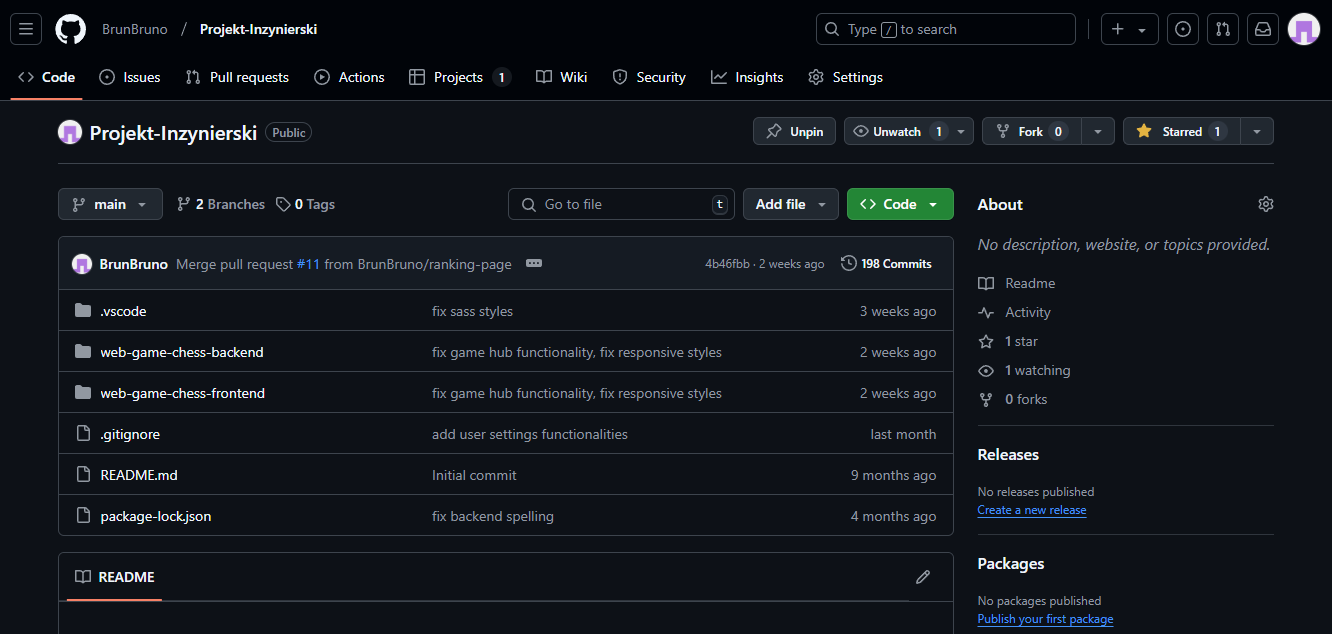
\includegraphics[width=1\textwidth]{images/gh_repo.png}
    \caption{Repozytorium na stronie github.com}
\end{figure}
\vspace{1cm}

\noindent 
Do wygodniejszej pracy z Git wykorzystany został program  \textbf{SourceTree}, czyli narzędzia desktopowego, które stanowi graficzny interfejs użytkownika do systemu Git. SourceTree pozwala na wygodne wywoływanie poleceń Git, takich jak commit, push, pull, czy merge w sposób bardziej intuicyjny i przystępny niż używanie terminala. Dzięki SourceTree zarządzanie gałęziami i wersjami jest bardzo proste i intuicyjne, a procesy takie jak przeglądanie historii commitów czy rozwiązywanie konfliktów w plikach są bardziej zorganizowane i mniej czasochłonne.

\newpage

\subsection{Warstwa danych}
\subsubsection{Opis architektury bazy danych}

Warstwa danych w aplikacji jest odpowiedzialna za zarządzanie przechowywaniem i dostępem do informacji w bazie danych. W omawianym projekcie wykorzystano system zarządzania bazą danych \textbf{PostgreSQL}, który jest jednym z najpopularniejszych rozwiązań bazodanowych o otwartym kodzie źródłowym. PostgreSQL charakteryzuje się dużą wydajnością, niezawodnością oraz elastycznością, co czyni go idealnym wyborem do obsługi wymagających aplikacji serwerowych.
\\\\
Z kolei do zarządzania interakcją z bazą danych w aplikacji serwerowej zastosowano bibliotekę \textbf{Entity Framework (EF)}. Entity Framework to popularny ORM (Object-Relational Mapping) dla .NET, który pozwala na mapowanie klas C\# na tabele w bazie danych, a także automatycznie generuje zapytania SQL na podstawie operacji na tych klasach. Dzięki EF, proces pracy z bazą danych jest znacznie uproszczony, ponieważ umożliwia on programistom operowanie na obiektach w aplikacji, a nie bezpośrednio na tabelach bazy danych.
\\\\
W tej aplikacji, każda encja (klasa reprezentująca dane) jest mapowana na odpowiednią tabelę w bazie danych, a właściwości tych klas odpowiadają kolumnom w tabelach. Dzięki temu, zapisane dane w postaci obiektów w aplikacji mogą być łatwo zapisywane i pobierane z bazy, co zapewnia spójność i łatwość w zarządzaniu danymi.
\\\\
Przykładowo, przy użyciu Entity Framework, klasy encji, które zostały zaprezentowane w dalszej części rozdziału, automatycznie generują odpowiednie tabele w bazie PostgreSQL. Ułatwia to pracę z danymi, pozwalając na ich łatwe przetwarzanie i manipulowanie, a jednocześnie zapewnia integralność danych w bazie.
\\\\
Do obsługi bazy danych, zarządzania danymi oraz monitorowania stanu bazy zastosowano narzędzie \textbf{PgAdmin}. Jest ono popularnym interfejsem graficznym dla PostgreSQL, który umożliwia łatwe zarządzanie bazą danych, tworzenie zapytań SQL, monitorowanie wydajności oraz przeprowadzanie operacji na danych, takich jak dodawanie, edytowanie czy usuwanie rekordów. Dzięki temu narzędziu możliwe jest szybkie i wygodne wykonywanie operacji administracyjnych oraz wgląd w strukturę bazy danych, co wspiera procesy rozwoju i utrzymania aplikacji.
\\\\
Poniżej zaprezentowane zostały diagramy \textbf{ERD (Entity-Relationship Diagram)}, które ilustrują strukturę bazy danych oraz relacje pomiędzy encjami. Każda z tych encji odpowiada za przechowywanie specyficznych danych, które są następnie wykorzystywane przez różne warstwy aplikacji w celu zapewnienia pełnej funkcjonalności systemu. Opis poszczególnych encji i ich zależności pozwala na lepsze zrozumienie, jak dane są przechowywane i powiązane w systemie.

\newpage

\subsubsection{Schemat bazy danych}

\noindent \textbf{Relacje użytkownika}\\
Segment relacji z użytkownikami obejmuje kilka encji i ich relacji, które zarządzają danymi użytkownika. Encja \textbf{\texttt{User}} jest rdzeniem tego segmentu i jest powiązany z wieloma innymi jednostkami. Każdy użytkownik jest powiązany z rolą, która definiuje uprawnienia użytkownika w systemie, a relacja między nimi jest ustanawiana za pomocą klucza obcego na \texttt{RoleId}. Ponadto każdy użytkownik jest powiązany z kodem weryfikacyjnym do celów weryfikacji w relacji ta jest jeden do jednego. Encje reprezentujące obrazy przechowują dane związane z zdjęciami, tworząc relacje jeden-do-jednego z podmiotem User. Jednostki odpowiadające za śledzenie ranking i statystyki użytkownika i są również powiązane z jednostką \texttt{User} poprzez relacje jeden-do-jednego. Sama jednostka \texttt{User} jest powiązana także z kilkoma innymi encjami łącząc pozostałem segment w jedną całość.

\vspace{1cm}
\begin{figure}[h!]
    \centering
    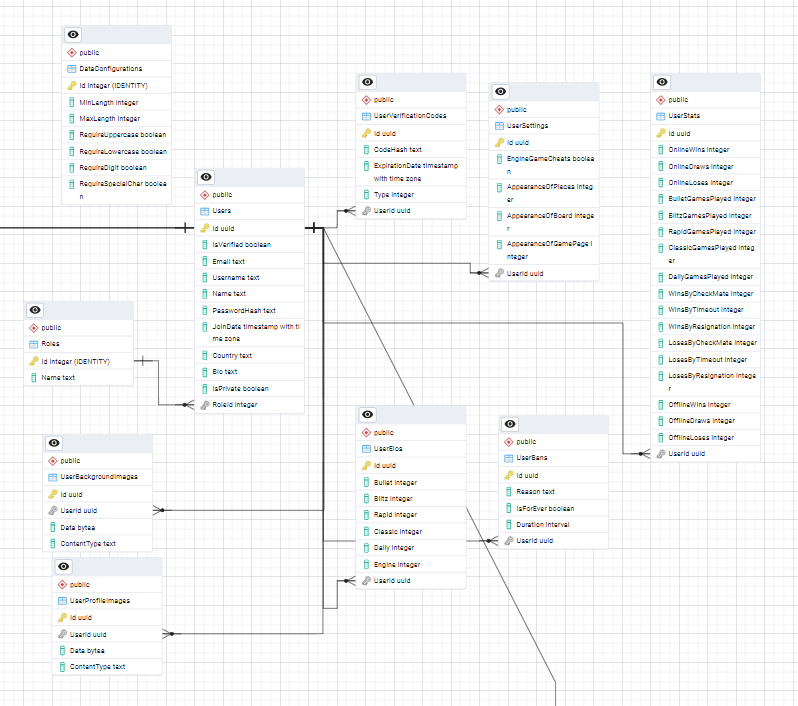
\includegraphics[width=0.9\textwidth]{images/ERD_user.png}
    \caption{Diagram relacji jednostka-relacja przedstawiający relacje użytkownika. Wygenerowany za pomocą programu PgAdmin.}
\end{figure}

\newpage

\noindent \textbf{Relacje znajomości}\\
Segment relacji przyjaźni jest zarządzany przez jednostkę przyjaźni, która reprezentuje połączenia społeczne między użytkownikami. Każda Encja \textbf{\texttt{Friendship}} ma dwóch kluczowych uczestników: \texttt{Requestor} (przyjmujacy) i \texttt{Receiver} (odbierający). Są to obaj użytkownicy, a relacje między tymi podmiotami są modelowane za pomocą kluczy obcych: \texttt{RequestorId} i \texttt{ReceiverId}. Ta relacja jest wiele-do-jednego, co oznacza, że użytkownik może mieć wiele przyjaźni zarówno jako żądający, jak i odbiorca. Dodatkowo, istnieje jednostka statystyk przyjaźni śledząca statystyki związane z każdą przyjaźnią, tworząc relację jeden-do-jednego z encją \texttt{Friendship}. Same znajomości są grupowane na podstawie pola \texttt{Status}, który jest wartością wyliczeniową, określającą rodzaj znajomości - są to relacje zaakceptowane, oczekujące i zablokowane.

\vspace{1cm}
\begin{figure}[h!]
    \centering
    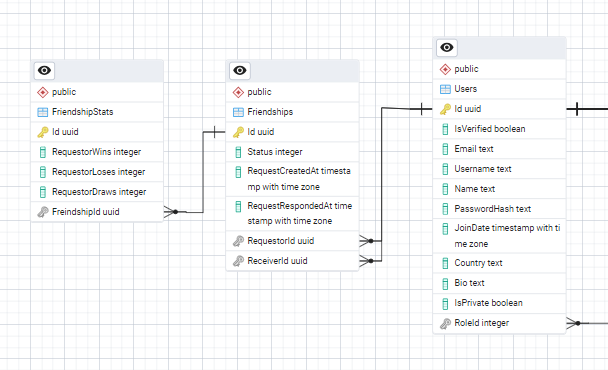
\includegraphics[width=0.9\textwidth]{images/ERD_friendship.png}
    \caption{Diagram relacji między podmiotami przedstawiający relacje przyjaźni między użytkownikami. Wygenerowany za pomocą programu PgAdmin.}
\end{figure}

\newpage

\noindent \textbf{Relacje w grach sieciowych}\\
Segment relacji gier online obsługuje strukturę internetowej gry w szachy, z kilkoma jednostkami, które śledzą różne aspekty gry. Jednostka \textbf{\texttt{WebGame}} jest główną w tym segmencie i reprezentuje samą grę, łącząc dwóch graczy poprzez relacje jeden-do-jednego. Stan i czas gry są kontrolowane przez osobne encje, które są połączone za pomocą kluczy obcych. Jednostka \texttt{WebGamePlayer} służy do zapisywania informacji specyficznych dla gracza i odwołuje się do jednostki \texttt{User} - użytkownik posiada wielu graczy. Ruchy wykonane w grze są przechowywane w osobnej tabli, która ma relację wiele do jednego z główną encję gry. Dodatkowo, wiadomości wymieniane podczas gry są obsługiwane przez encje dwa osobne obiekty, tworzące relacje wiele-do-jednego odpowiednio z encjami samej gry jak i gracza.

\vspace{1cm}
\begin{figure}[h!]
    \centering
    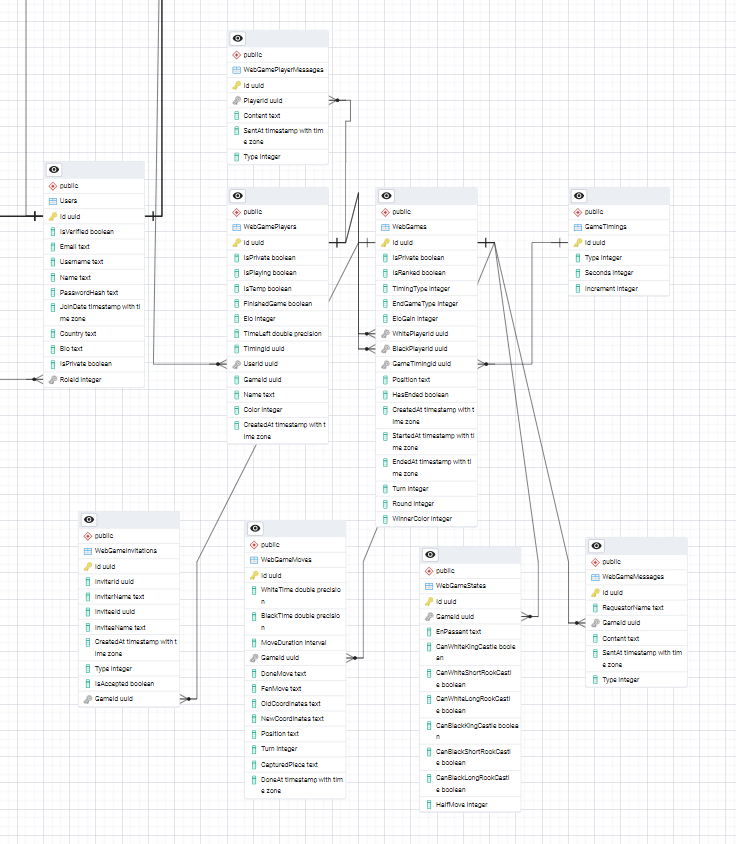
\includegraphics[width=0.9\textwidth]{images/ERD_online.png}
    \caption{Diagram relacji między podmiotami ilustrujący strukturę interakcji w grach sieciowych. Wygenerowany za pomocą programu PgAdmin.}
\end{figure}

\newpage

\noindent \textbf{Relacje w grach z silnikiem}\\
Segment ten skupia się na aspekcie gry opartym na silniku, gdzie każda gra jest zarządzana przez encję \textbf{\texttt{EngineGame}}. Encja ta jest powiązana z encją gracza, reprezentującą użytkownika, który gra w grę opartą na silniku, a relacja jeden-do-jednego jest ustanawiana poprzez parametr \texttt{PlayerId}. Każdy ruch w grze jest przechwytywany w tabeli ruchów, która jest powiązana z główną encją poprzez klucz obcy. Encja stanu gry przechowuje aktualny stan gry opartej na silniku i jest powiązana z \texttt{EngineGame} poprzez relację jeden-do-jednego. Dodatkowo, wiadomości specyficzne dla gier silnikowych są przechowywane w osobnej liscie obiektów, która jest powiązana z \texttt{EngineGame} poprzez klucz obcy.

\vspace{1cm}
\begin{figure}[h!]
    \centering
    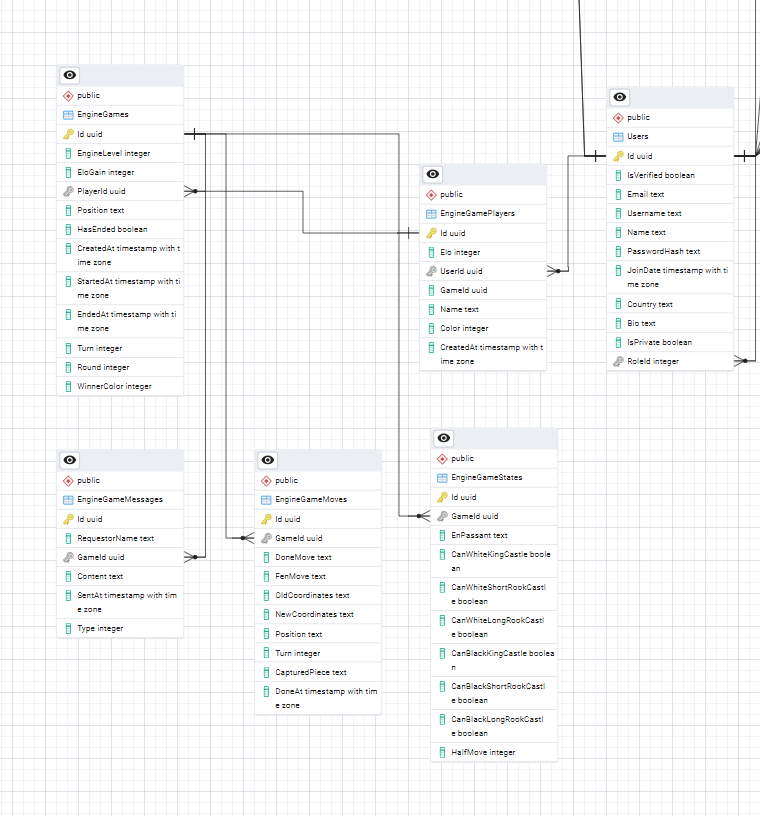
\includegraphics[width=0.9\textwidth]{images/ERD_offline.png}
    \caption{Diagram zależności między jednostkami przedstawiający relacje między silnikiem a grą. Wygenerowany za pomocą programu PgAdmin.}
\end{figure}

\newpage


\subsubsection{Opis encji}
W ramach warstwy danych aplikacji, encje pełnią kluczową rolę w odwzorowywaniu struktury danych, które są przechowywane w bazie danych. W tym rozdziale przedstawione zostały wszystkie encje projektu, ich właściwości oraz powiązania między nimi. Każda z encji odpowiada za przechowywanie danych dotyczących określonych elementów systemu, takich jak użytkownicy, gry czy relacje, a ich odpowiedniki w bazie danych są realizowane za pomocą tabel.
\\\\
Ważnym aspektem w projekcie jest wykorzystanie klas abstrakcyjnych, które stanowią wspólne podstawy dla encji reprezentujących różne, ale podobne obiekty w systemie. Klasy abstrakcyjne nie mają swojego odwzorowania w bazie danych, jednak pełnią rolę pośredników, umożliwiając dziedziczenie i tworzenie bardziej specyficznych encji. Na przykład, encje reprezentujące gry online oraz gry z komputerem dziedziczą po klasach abstrakcyjnych, które definiują wspólne właściwości dla wszystkich gier. Jednak szczegóły, takie jak obecność kontroli czasu, różnią się w zależności od typu gry — gry online mogą mieć kontrolę czasu, podczas gdy gry offline nie.
\\\\
W samych encjach zdefiniowane są również powiązania z innymi encjami, które realizowane są przez klucze obce. Klucze obce są zapisane jako kolumny w tabelach, przyjmujące postać identyfikatorów powiązanych encji. Dzięki temu możliwe jest tworzenie odpowiednich relacji pomiędzy danymi w różnych tabelach. W przypadku relacji jeden do wielu, zastosowanie znajdują listy, które umożliwiają przypisanie wielu obiektów do jednej encji.
\\\\
Encje w projekcie zostały podzielone logicznie, zgodnie z rolą, jaką pełnią w systemie. Na przykład, encja użytkownika (User) jest powiązana z encją punktacji, jednak punktacja jest przechowywana w osobnej tabeli, ponieważ jest uzywana do konkretnych, innych funkcjonalności niż sam User. Dzięki takiemu podziałowi możliwe jest bardziej elastyczne zarządzanie danymi oraz lepsze odwzorowanie relacji pomiędzy różnymi elementami systemu.
\\\\
Poniżej zaprezentowano encje abstrakcyjne oraz te, które mają swoje odzwierciedlenie w bazie danych, z pominięciem abstrakcyjnych wartości. Dzięki temu możliwe jest zobrazowanie rzeczywistej struktury danych, które są przechowywane w systemie, oraz przedstawienie relacji między różnymi encjami, które są kluczowe dla prawidłowego funkcjonowania aplikacji.

\newpage

\textbf{Abstrakcyjne jednostki}\\

\begin{itemize}
    \item \textbf{Game}\\
    Klasa dziedziczona przez podmioty reprezentujące gry Deklaruje podstawowe właściwości jakie powinna posiadać każda gra.
    \renewcommand{\arraystretch}{1.5}
    \begin{longtable}{|m{4cm}|m{2cm}|m{8cm}|}
        \hline
        \rowcolor{lightgray}
        \textbf{Właściwość} & \textbf{Typ} & \textbf{Opis} \\ \hline
        \endhead
        \hline
        Position & string & Aktualna pozycja na szachownicy w formacie FEN \\ \hline
        HasEnded & bool & Flaga, czy gra się zakończyła \\ \hline
        CreatedAt & DateTime & Data utworzenia gry \\ \hline
        StartedAt & DateTime? & Data rozpoczęcia gry \\ \hline
        EndedAt & DateTime? & Data zakończenia gry \\ \hline
        Turn & int & Numer tury gry \\ \hline
        Round & int & Numer rundy \\ \hline
        WinnerColor & enum? & Kolor zwycięzcy (null oznacza remis) \\ \hline
    \end{longtable}

    \item \textbf{Player}\\
    Generalna klasa przechowują podstawowe dane reprezentujące gracza.
    \renewcommand{\arraystretch}{1.5}
    \begin{longtable}{|m{4cm}|m{2cm}|m{8cm}|}
        \hline
        \rowcolor{lightgray}
        \textbf{Właściwość} & \textbf{Typ} & \textbf{Opis} \\ \hline
        \endhead
        \hline
        Name & string & Nazwa gracza (nazwa użytkownika) \\ \hline
        Color & enum? & Kolor gracza (czarny lub biały), null jeśli gracz szuka jeszcze gry \\ \hline
        CreatedAt & DateTime & Data utworzenia gracza \\ \hline
    \end{longtable}

    \item \textbf{GameState}\\
    Abstrakcyjna encja reprezentująca stan gry, zawierająca szczegółowe informacje, ktorych nie ma sposobu pozyskać w inny wypadku, niż poprzez zapisanie wystąpienia zdarzenia. Dotyczy głównie ruchów specjalnych, charakteryzujących się wieloma zasadami.
    \renewcommand{\arraystretch}{1.5}
    \begin{longtable}{|m{4cm}|m{2cm}|m{8cm}|}
        \hline
        \rowcolor{lightgray}
        \textbf{Właściwość} & \textbf{Typ} & \textbf{Opis} \\ \hline
        \endhead
        \hline
        EnPassant & string? & Koordynaty dla specjalnego bicia en passant w formacie "x,y" \\ \hline
        (Can castle) & bool & Pola określające, czy gracze mogą wykonać roszadę \\ \hline
        HalfMove & int & Liczba ruchów nie będących ruchem pionkiem (dla zasady 50 ruchów) \\ \hline
    \end{longtable}

\newpage

    \item \textbf{Move}\\
    Abstrakcyjna encja przedstawiająca ruch wykonany podczas rozgrywki. Jednoznacznie identyfikuje informacje o stanie gry po wykonaniu ruchu podczas gry.
    \renewcommand{\arraystretch}{1.5}
    \begin{longtable}{|m{4cm}|m{2cm}|m{8cm}|}
        \hline
        \rowcolor{lightgray}
        \textbf{Właściwość} & \textbf{Typ} & \textbf{Opis} \\ \hline
        \endhead
        \hline
        DoneMove & string & Wykonany ruch w formacie: tag figury + x (jeśli zbicie) + współrzędne xy \\ \hline
        FenMove & string & Wykonany ruch w formacie FEN \\ \hline
        OldCoordinates & string & Współrzędne, z których figura została przemieszczona w formacie x,y \\ \hline
        NewCoordinates & string & Współrzędne, na które figura została przemieszczona w formacie x,y \\ \hline
        Position & string & Pozycja na szachownicy po wykonaniu ruchu \\ \hline
        Turn & int & Tura, w której ruch został wykonany \\ \hline
        CapturedPiece & string? & Tag zbitej figury \\ \hline
        DoneAt & DateTime & Data i godzina wykonania ruchu \\ \hline
    \end{longtable}

    \item \textbf{Message}\\
    Generalna encja reprezentująca wiadomości tworzone podczas gry (automatycznie i poprzez użytkowników).
    \renewcommand{\arraystretch}{1.5}
    \begin{longtable}{|m{4cm}|m{2cm}|m{8cm}|}
        \hline
        \rowcolor{lightgray}
        \textbf{Właściwość} & \textbf{Typ} & \textbf{Opis} \\ \hline
        \endhead
        \hline
        Content & string & Treść wiadomości \\ \hline
        SentAt & DateTime & Data i godzina wysłania wiadomości \\ \hline
        Type & enum & Typ wiadomości (automatyczna / wysłana) \\ \hline
    \end{longtable}

    \item \textbf{Image}\\
    Abstrakcyjna klasa reprezentująca pliki graficzne.
    \renewcommand{\arraystretch}{1.5}
    \begin{longtable}{|m{4cm}|m{2cm}|m{8cm}|}
        \hline
        \rowcolor{lightgray}
        \textbf{Właściwość} & \textbf{Typ} & \textbf{Opis} \\ \hline
        \endhead
        \hline
        Data & byte[] & Dane obrazu w postaci bajtów \\ \hline
        ContentType & string & Typ zawartości obrazu (np. "image/png", "image/jpeg") \\ \hline
    \end{longtable}
\end{itemize}

\newpage

\textbf{Tabele bazy danych}\\

\begin{itemize}
    \item \textbf{DataConfigurations}\\
    Zawiera ustawienia konfiguracji dla kluczowych pól użytkownika (takie jak hasło i nazwa użytkownika). Nie jest powiązana z żadną inną jednostką.

    \item \textbf{Roles}\\
    Określa role użytkowników w systemie, takie jak "User" i "Admin".

    \item \textbf{Users}\\
    Główna encja reprezentująca użytkownika.
    \renewcommand{\arraystretch}{1.5}
    \begin{longtable}{|m{4cm}|m{2cm}|m{8cm}|}
        \hline
        \rowcolor{lightgray}
        \textbf{Właściwość} & \textbf{Typ} & \textbf{Opis} \\ \hline
        \endhead
        \hline
        Id & Guid & Identyfikator użytkownika (PK) \\ \hline
        IsVerified & bool & Flaga określająca czy email użytkownika jest zweryfikowany \\ \hline
        IsPrivate & bool & Określa, czy profil użytkownika jest widoczny przez innych użytkowników \\ \hline
        Email & string & Adres email użytkownika \\ \hline
        Username & string & Unikalna nazwa użytkownika \\ \hline
        Name & string? & Opcjonalne pełne imię i nazwisko \\ \hline
        PasswordHash & string & Zahashowane hasło użytkownika \\ \hline
        JoinDate & DateTime & Data dołączenia użytkownika do systemu \\ \hline
        Country & string & Kraj, w którym użytkownik się zarejestrował \\ \hline
        Bio & string? & Krótkie bio lub opis użytkownika \\ \hline
        RoleId & int & Identyfikator roli użytkownika\\ \hline
    \end{longtable}

    \item \textbf{UserVerificationCodes}\\
    Tablica kodów weryfikacyjnych. Kody dzielą się na dwa typy, ze względu na rodzaj przeznaczenia - dotyczące weryfikacji kota oraz odzyskiwania hasła.
    \renewcommand{\arraystretch}{1.5}
    \begin{longtable}{|m{4cm}|m{2cm}|m{8cm}|}
        \hline
        \rowcolor{lightgray}
        \textbf{Właściwość} & \textbf{Typ} & \textbf{Opis} \\ \hline
        \endhead
        \hline
        Id & Guid & Identyfikator kodu weryfikacyjnego (PK) \\ \hline
        CodeHash & string & Zahashowany kod używany do weryfikacji \\ \hline
        ExpirationDate & DateTime & Data wygaśnięcia kodu weryfikacyjnego \\ \hline
        Type & enum & Typ kodu weryfikacyjnego \\ \hline
        UserId & Guid & Identyfikator użytkownika, do którego należy kod weryfikacyjny \\ \hline
    \end{longtable}

\newpage

    \item \textbf{UserElos}\\
    Punktacja użytkownika dla poszczególnych trybów czasowych gry.
    \renewcommand{\arraystretch}{1.5}
    \begin{longtable}{|m{4cm}|m{2cm}|m{8cm}|}
        \hline
        \rowcolor{lightgray}
        \textbf{Właściwość} & \textbf{Typ} & \textbf{Opis} \\ \hline
        \endhead
        \hline
        Id & Guid & Identyfikator ELO (PK) \\ \hline
        (Kategorii kontroli) & int & Punkty ELO dla konkretnego trybu kontroli czasowej \\ \hline
        UserId & Guid & Identyfikator użytkownika, do którego należy punktacja \\ \hline
    \end{longtable}

    \item \textbf{UserStats}\\
    Tablica statystyki użytkownika.
    \renewcommand{\arraystretch}{1.5}
    \begin{longtable}{|m{4cm}|m{2cm}|m{8cm}|}
        \hline
        \rowcolor{lightgray}
        \textbf{Właściwość} & \textbf{Typ} & \textbf{Opis} \\ \hline
        \endhead
        \hline
        Id & Guid & Identyfikator statystyk użytkownika (PK) \\ \hline
        (Statystyki gier) & int & Zawiera różnorodne dane liczbowe dotyczące gier użytkownika, takie jak wygrane, przegrane, remisy, liczba rozegranych gier w różnych trybach oraz inne wskaźniki wyników \\ \hline
        UserId & Guid & Identyfikator użytkownika, do którego należą statystyki \\ \hline
    \end{longtable}
        
    \item \textbf{UserSettings}\\
    Globalne ustawienia konta oraz gier.
    \renewcommand{\arraystretch}{1.5}
    \begin{longtable}{|m{4cm}|m{2cm}|m{8cm}|}
        \hline
        \rowcolor{lightgray}
        \textbf{Właściwość} & \textbf{Typ} & \textbf{Opis} \\ \hline
        \endhead
        \hline
        Id & Guid & Identyfikator ustawień użytkownika (PK) \\ \hline
        (Ustawienia gry) & enum, bool & Określa ustawienia dotyczące gry z silnikiem oraz spersonalizowane ustawienia wyglądu strony \\ \hline
        UserId & Guid & Identyfikator użytkownika, do którego należą ustawienia \\ \hline
    \end{longtable}

    \item \textbf{UserProfileImage oraz UserBackgroundImages}\\
    zdjęcia użytkownika. Powiązane w relacja jeden-do-jeden z użytkownikiem. Dziedziczą po klasie abstrakcyjnej \texttt{Image}, reprezentującą zdjęcia zapisane w bazie.
    \renewcommand{\arraystretch}{1.5}
    \begin{longtable}{|m{4cm}|m{2cm}|m{8cm}|}
        \hline
        \rowcolor{lightgray}
        \textbf{Właściwość} & \textbf{Typ} & \textbf{Opis} \\ \hline
        \endhead
        \hline
        Id & Guid & Identyfikator obrazu (PK) \\ \hline
        UserId & Guid & Identyfikator użytkownika, do którego należy zdjęcie \\ \hline
    \end{longtable}

\newpage

    \item \textbf{Friendships}\\
    Tablica relacji pomiędzy użytkownikami.
    \renewcommand{\arraystretch}{1.5}
    \begin{longtable}{|m{4cm}|m{2cm}|m{8cm}|}
        \hline
        \rowcolor{lightgray}
        \textbf{Właściwość} & \textbf{Typ} & \textbf{Opis} \\ \hline
        \endhead
        \hline
        Id & Guid & Identyfikator relacji przyjaźni (PK) \\ \hline
        Status & enum & Status przyjaźni  \\ \hline
        RequestCreatedAt & DateTime & Data utworzenia/złożenia wniosku o przyjaźń \\ \hline
        RequestRespondedAt & DateTime? & Data, kiedy druga strona odpowiedziała na wniosek o przyjaźń \\ \hline
        RequestorId & Guid & Identyfikator użytkownika, który wysłał prośbę o przyjaźń \\ \hline
        ReceiverId & Guid & Identyfikator użytkownika, który otrzymał prośbę o przyjaźń \\ \hline
    \end{longtable}

    \item \textbf{FriendshipStats}\\
    Statystki dotyczące relacji uzytkownikow.
    \renewcommand{\arraystretch}{1.5}
    \begin{longtable}{|m{4cm}|m{2cm}|m{8cm}|}
        \hline
        \rowcolor{lightgray}
        \textbf{Właściwość} & \textbf{Typ} & \textbf{Opis} \\ \hline
        \endhead
        \hline
        Id & Guid & Identyfikator statystyk przyjaźni (PK) \\ \hline
        RequestorWins & int & Liczba wygranych gier użytkownika inicjującego relację \\ \hline
        RequestorLoses & int & Liczba przegranych gier użytkownika inicjującego relację \\ \hline
        RequestorDraws & int & Liczba remisów gier użytkownika inicjującego relację \\ \hline
        GamesPlayed & int & Całkowita liczba gier rozegranych w relacji (suma wygranych, przegranych i remisów) \\ \hline
        FriendshipId & Guid & Identyfikator relacji przyjaźni, do której należą statystyki \\ \hline
        Friendship & Friendship & Obiekt reprezentujący szczegóły relacji przyjaźni \\ \hline
    \end{longtable}
  
\newpage
    
    \item \textbf{WebGames}\\
    Gry online między użytkownikami. Każda gra zawiera powiązanie do dwóch gracz - oznaczonego jako białego i czarnego w zależności od strony jaką przyjmują. WebGame dziedziczy po abstrakcyjnej klasie gry.
    \renewcommand{\arraystretch}{1.5}
    \begin{longtable}{|m{4cm}|m{2cm}|m{8cm}|}
        \hline
        \rowcolor{lightgray}
        \textbf{Właściwość} & \textbf{Typ} & \textbf{Opis} \\ \hline
        \endhead
        \hline
        Id & Guid & Identyfikator gry online (PK) \\ \hline
        IsPrivate & bool & Określa, czy gra jest prywatna czy publiczna \\ \hline
        IsRanked & bool & Określa, czy gra będzie miała wpływ na ranking Elo \\ \hline
        TimingType & enum & Typ czasu gry (np. Bullet, Blitz, Rapid) \\ \hline
        EndGameType & enum? & Powód zakończenia gry (np. mat, czas) \\ \hline
        EloGain & int & Zysk lub strata Elo po zakończeniu gry \\ \hline
        WhitePlayerId & Guid & Identyfikator gracza grającego białymi \\ \hline
        BlackPlayerId & Guid & Identyfikator gracza grającego czarnymi \\ \hline
        GameTimingId & Guid & Identyfikator ustawień czasu gry \\ \hline
    \end{longtable}

    \item \textbf{WebGamePlayers}\\
    Tablica graczy gry online, reprezentujące użytkownika jako gracza należącego do gry. Dziedziczy po klasie Player oraz zawiera dodatkowe elementy, ze względu an czasowy charakter gry.
    \renewcommand{\arraystretch}{1.5}
    \begin{longtable}{|m{4cm}|m{2cm}|m{8cm}|}
        \hline
        \rowcolor{lightgray}
        \textbf{Właściwość} & \textbf{Typ} & \textbf{Opis} \\ \hline
        \endhead
        \hline
        Id & Guid & Identyfikator gracza (PK) \\ \hline
        IsPrivate & bool & Określa, czy gracz może być używany w globalnym wyszukiwaniu, czy jest tylko dla prywatnej gry \\ \hline
        IsPlaying & bool & Flaga, czy gracz wciąż szuka gry \\ \hline
        IsTemp & bool & Flaga, czy gracz jest tymczasowy \\ \hline
        FinishedGame & bool & Flaga, czy gra dla gracza została zakończona \\ \hline
        Elo & int & Punkty Elo dla konkretnego typu czasu \\ \hline
        TimeLeft & double & Czas pozostały na wykonanie ruchów zgodnie z czasem gry \\ \hline
        TimingId & Guid & Id typu czasu, określający czas trwania i przyrost czasu dla wszystkich ruchów \\ \hline
        UserId & Guid & Id użytkownika, któremu gracz należy \\ \hline
        GameId & Guid & Id gry, w której gracz bierze udział \\ \hline
    \end{longtable}
 
\newpage

    \item \textbf{GameTimings}\\
    Kontrole czasowe dla gier z ograniczeniem czasu. Kontrola czasowa jest powiązana w grami w relacji jeden do wielu, co oznacza, że jeden rodzaj kontroli jest wykorzystywany w wielu grach.
    \renewcommand{\arraystretch}{1.5}
    \begin{longtable}{|m{4cm}|m{2cm}|m{8cm}|}
        \hline
        \rowcolor{lightgray}
        \textbf{Właściwość} & \textbf{Typ} & \textbf{Opis} \\ \hline
        \endhead
        \hline
        Id & Guid & Identyfikator ustawienia czasu gry (PK) \\ \hline
        Type & enum & Kategoria (typ) kontroli czasu (np. Bullet, Rapid) \\ \hline
        Seconds & int & Czas trwania gry w sekundach \\ \hline
        Increment & int & Inkrement czasowy w sekundach \\ \hline
    \end{longtable}

    \item \textbf{WebGameStates}\\
    Stan gry online, przechowuje dane szczególne dotyczące obecnej gry. Dziedziczy w abstrakcyjnej klasie stanów gry.
    
    \item \textbf{WebGameInvitations}\\
    Opcjonalne zaproszenia do gry. Generowane tylko do gier prywatach i służące do mechanizmów związanych z zapraszaniem do gry i odpowiedziami na zaproszenia.
    \renewcommand{\arraystretch}{1.5}
    \begin{longtable}{|m{4cm}|m{2cm}|m{8cm}|}
        \hline
        \rowcolor{lightgray}
        \textbf{Właściwość} & \textbf{Typ} & \textbf{Opis} \\ \hline
        \endhead
        \hline
        Id & Guid & Identyfikator zaproszenia (PK) \\ \hline
        InviterId & Guid & Identyfikator użytkownika zapraszającego \\ \hline
        InviteeId & Guid & Identyfikator użytkownika zapraszanego \\ \hline
        InviterName & string & Nazwa użytkownika zapraszającego do relacji \\ \hline
        InviteeName & string & Nazwa użytkownika zaproszonego do relacji \\ \hline
        CreatedAt & DateTime & Data utworzenia zaproszenia \\ \hline
        Type & enum & Typ kontroli czasowej \\ \hline
        IsAccepted & bool & Flaga, która wskazuje, czy zaproszenie zostało zaakceptowane \\ \hline
        GameId & Guid & Id gry, do której należy zaproszenie \\ \hline
    \end{longtable}

\newpage

    \item \textbf{WebGameMove}\\
    Ruchy wykonane podczas gry online. Dziedziczy po klasie Move, a dodatkowo ze względu na kontrole czasową występującą w grach między użytkownikami zawiera pola związane z czasem.
    \renewcommand{\arraystretch}{1.5}
    \begin{longtable}{|m{4cm}|m{2cm}|m{8cm}|}
        \hline
        \rowcolor{lightgray}
        \textbf{Właściwość} & \textbf{Typ} & \textbf{Opis} \\ \hline
        \endhead
        \hline
        Id & Guid & Identyfikator ruchu (PK) \\ \hline
        WhiteTime & double & Czas pozostały dla białego gracza \\ \hline
        BlackTime & double & Czas pozostały dla czarnego gracza \\ \hline
        MoveDuration & TimeSpan & Czas, który gracz zużył na wykonanie ruchu \\ \hline
        GameId & Guid & Identyfikator gry, do której ruch należy \\ \hline
    \end{longtable}
        
    \item \textbf{WebGameMessages}\\
    Wiadomości systemowe dotyczące gry online. Otrzymują własności po generalnej klasnie reprezentującą wiadomości. 
    \renewcommand{\arraystretch}{1.5}
    \begin{longtable}{|m{4cm}|m{2cm}|m{8cm}|}
        \hline
        \rowcolor{lightgray}
        \textbf{Właściwość} & \textbf{Typ} & \textbf{Opis} \\ \hline
        \endhead
        \hline
        Id & Guid & Identyfikator ruchu (PK) \\ \hline
        GameId & Guid & Identyfikator gry, do której wiadomość należy \\ \hline
    \end{longtable}

    \item \textbf{WebGamePlayerMessages}\\
    Wiadomości wysłane przez graczy podczas gry online. Dziedziczą wartości po abstrakcyjnej klasie Message.
    \renewcommand{\arraystretch}{1.5}
    \begin{longtable}{|m{4cm}|m{2cm}|m{8cm}|}
        \hline
        \rowcolor{lightgray}
        \textbf{Właściwość} & \textbf{Typ} & \textbf{Opis} \\ \hline
        \endhead
        \hline
        Id & Guid & Identyfikator ruchu (PK) \\ \hline
        PlayerId & Guid & Identyfikator gracza, do którego wiadomość należy \\ \hline
    \end{longtable}
        
\newpage

    \item \textbf{EngineGames}\\
    Tablica gier offline z silnikiem szachowym. Dziedziczy także podobnie jak w przypadku gier online po abstrakcyjnej klasie Game.  
    \renewcommand{\arraystretch}{1.5}
    \begin{longtable}{|m{4cm}|m{2cm}|m{8cm}|}
        \hline
        \rowcolor{lightgray}
        \textbf{Właściwość} & \textbf{Typ} & \textbf{Opis} \\ \hline
        \endhead
        \hline
        Id & Guid & Identyfikator gry (PK) \\ \hline
        EngineLevel & int & Poziom głębokości silnika \\ \hline
        EloGain & int & Zysk lub strata Elo po zakończeniu gry \\ \hline
        PlayerId & Guid & Identyfikator gracza \\ \hline
    \end{longtable}
    
    \item \textbf{EngineGameStates}\\
    Stan gry offline, przechowuje dane szczególne dotyczące obecnej gry. Implementuje własności z abstrakcyjnej klasy stanów gry.

    \item \textbf{EngineGamePlayers}\\
    Gracze gier offline, reprezentujące użytkownika jako gracza w grze z silnikiem szachowym. Dziedziczy podstawowe dane po klasie Player.
    \renewcommand{\arraystretch}{1.5}
    \begin{longtable}{|m{4cm}|m{2cm}|m{8cm}|}
        \hline
        \rowcolor{lightgray}
        \textbf{Właściwość} & \textbf{Typ} & \textbf{Opis} \\ \hline
        \endhead
        \hline
        Id & Guid & Identyfikator gracza (PK) \\ \hline
        Elo & int & Punkty Elo dla gier przeciwko silnikowi \\ \hline
        UserId & Guid & Identyfikator użytkownika, do którego należy gracz \\ \hline
        GameId & Guid & Identyfikator gry, w której gracz bierze udział \\ \hline
    \end{longtable}
    
    \item \textbf{EngineGameMoves}\\
    Ruchy wykonane podczas gry offline. Dziedziczą po abstrakcyjnej klasie ruchu oraz nie implementują żadnych własnych właściwości.
    \renewcommand{\arraystretch}{1.5}
    \begin{longtable}{|m{4cm}|m{2cm}|m{8cm}|}
        \hline
        \rowcolor{lightgray}
        \textbf{Właściwość} & \textbf{Typ} & \textbf{Opis} \\ \hline
        \endhead
        \hline
        Id & Guid & Identyfikator ruchu (PK) \\ \hline
        GameId & Guid & Identyfikator gry, do której ruch należy \\ \hline
    \end{longtable}
    
    \item \textbf{EngineGameMessages}\\
    Automatyczne wiadomości dotyczące gry offline. Zaprojektowane identycznie jak w przypadku wiadomości aromatycznych gie online.
    
\end{itemize}

\newpage

\subsection{Warstwa Serwerowa (Backend)} 
\subsubsection{Architektura i struktura} 
Architektura backendu została zaprojektowana w oparciu o podejście \textbf{Onion Architecture}, które promuje modularność, odwrócenie zależności oraz izolację logiki biznesowej od infrastruktury. Główne założenia tej architektury koncentrują się na umożliwieniu rozwoju aplikacji w sposób niezależny od technologii, co sprzyja łatwemu utrzymaniu oraz skalowaniu systemu. Struktura projektu jest podzielona na kilka warstw, które komunikują się ze sobą poprzez jasno zdefiniowane kontrakty i interfejsy. Kluczowym celem tego podejścia jest ochrona rdzenia aplikacji przed zmianami w zewnętrznych technologiach i zależnościach, co pozwala na łatwiejsze dostosowywanie aplikacji do nowych wymagań i technologii.

\begin{figure}[h!] 
    \centering 
    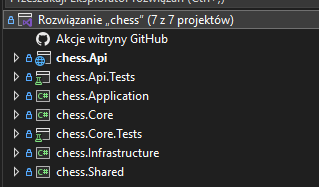
\includegraphics[width=0.7\textwidth]{images/struktura_back.png} 
    \caption{Struktura projektów solucji warstwy serwerowej.} 
\end{figure}

\noindent \textbf{Zalety Onion Architecture:}
\begin{itemize}
    \item \textbf{Izolacja logiki biznesowej:} pozwala na pełną separację logiki biznesowej od zewnętrznych zależności, co umożliwia łatwe testowanie i modyfikowanie samej logiki bez wpływu na resztę systemu.
    \item \textbf{Skalowalność i elastyczność:} modularność struktury pozwala na łatwą rozbudowę systemu, poprzez dodawanie nowych warstw lub rozszerzanie istniejących komponentów bez ryzyka wprowadzenia chaosu w kodzie.
    \item \textbf{Testowalność:} dzięki wyodrębnieniu warstw odpowiedzialnych za różne aspekty systemu, testowanie staje się prostsze i bardziej zorganizowane, ponieważ możemy testować poszczególne warstwy niezależnie.
    \item \textbf{Odwrócenie zależności:} warstwa zewnętrzna może korzystać z funkcjonalności warstw wewnętrznych, ale nie odwrotnie. To oznacza, że zmiany w bazach danych czy frameworkach nie wpływają na kluczową logikę biznesową aplikacji.
\end{itemize}

\noindent
Podejście to pozwala na przejrzystość w organizacji kodu, ułatwiając zarządzanie projektem i współpracę zespołową. Dzięki jasnemu podziałowi na warstwy, każdy członek zespołu może skupić się na odpowiednim obszarze aplikacji, bez konieczności przyswajania całościowej struktury systemu. Dodatkowo, umożliwia łatwe przeprowadzanie migracji technologicznych w obrębie poszczególnych warstw, minimalizując ryzyko wprowadzenia błędów w działającej aplikacji.

\newpage

\noindent
Zależności między poszczególnymi modułami zaprezentowane zostały za pomocą grafu, co pozwala na wizualizację i lepsze zrozumienie interakcji między warstwami. Graf ten odzwierciedla zasady Onion Architecture, w której zależności zawsze kierują się do wewnątrz, tj. od warstw zewnętrznych do bardziej wewnętrznych.
\\\\
Moduł .Api zależy wyłącznie od warstwy .Application, co oznacza, że obsługuje żądania i deleguje ich przetwarzanie do przypadków użycia w Application. Z kolei .Application komunikuje się z modułem .Core, który definiuje kluczowe modele domenowe. Warstwa .Core pozostaje całkowicie niezależna od innych modułów, co jest zgodne z zasadami odwrócenia zależności.
\\
Moduł .Infrastructure implementuje interfejsy zdefiniowane w .Application, dostarczając szczegóły techniczne, takie jak integracje czy dostęp do danych, ale nie wymusza zależności zwrotnej na rdzeniu. .Shared działa jako pomocniczy moduł, który może być używany przez dowolną warstwę, dostarczając wspólny kod i narzędzia.

\begin{figure}[h!]
    \centering
    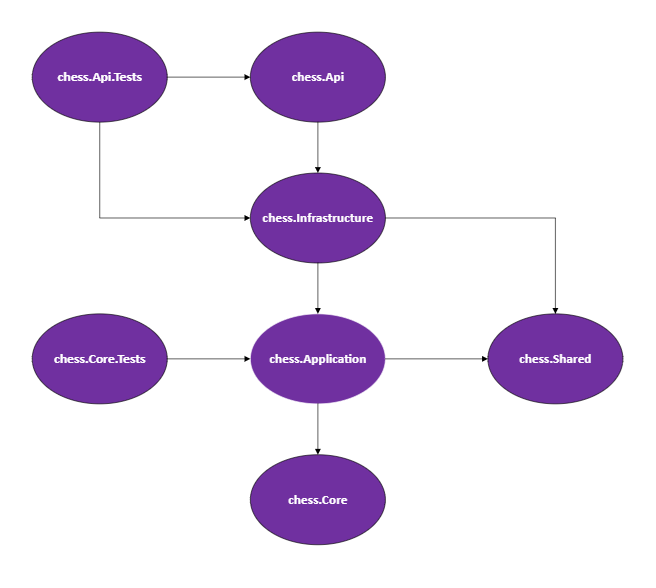
\includegraphics[width=1\textwidth]{images/diagram_dependencies.png}
    \caption{Diagram zależności między projektami. Opracowany za pomocą aplikacji Viso.}
\end{figure}

\newpage

\noindent \textbf{Warstwa prezentacji}\\
Moduł \textbf{.Api} pełni funkcję warstwy zewnętrznej, odpowiedzialnej za obsługę żądań HTTP oraz przekazywanie ich do odpowiednich komponentów logiki aplikacji. Jest to punkt wejściowy dla użytkowników lub zewnętrznych integracji. Warstwa ta korzysta z usług dostarczanych przez moduł Application, pozostając przy tym niezależna od szczegółów implementacyjnych niższych warstw.

\vspace{0.5cm}
\begin{minipage}[t]{0.45\textwidth}
    \vspace{0pt}
    \raggedright
    Warstwa prezentacji odpowiada za obsługę komunikacji zewnętrznej aplikacji, interpretację żądań od użytkowników oraz ich przekazywanie do warstw logiki aplikacyjnej. Zawiera kontrolery realizujące logikę obsługi poszczególnych zasobów oraz huby, takie jak SignalR Hub, które obsługują komunikację w czasie rzeczywistym. Modele w tym module reprezentują dane odbierane z endpointów aplikacji. Mapy przekształcają te modele na żądania odpowiadające wymaganiom warstwy aplikacyjnej. Moduł zapewnia również mechanizmy autoryzacji, umożliwiające kontrolę dostępu do zasobów i operacji w systemie.
\end{minipage}
\hfill
\begin{minipage}[t]{0.45\textwidth}
    \vspace{0pt}
    \centering
    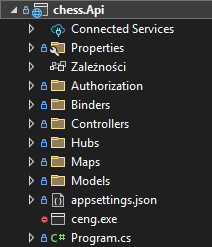
\includegraphics[width=\linewidth]{images/struktura_back_api.png}
\end{minipage}
\vspace{0.5cm}

\noindent \textbf{Warstwa aplikacji}\\
Moduł \textbf{.Application} zawiera logikę aplikacyjną, w tym definicje przypadków użycia, które realizują wymagania systemowe. Jest on pośrednikiem między warstwą interfejsu (Api) a rdzeniem systemu, reprezentowanym przez moduł Core. Dzięki temu logika biznesowa jest chroniona przed szczegółami technicznymi, takimi jak sposób przetwarzania żądań czy dostęp do danych.

\vspace{0.5cm}
\begin{minipage}[t]{0.45\textwidth}
    \vspace{0pt}
    \centering
    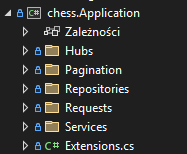
\includegraphics[width=\linewidth]{images/struktura_back_application.png} 
\end{minipage}
\hfill
\begin{minipage}[t]{0.45\textwidth}
    \vspace{0pt}
    \raggedright
    Warstwa aplikacji łączy warstwy zewnętrzne z rdzeniem systemu. Zawiera interfejsy dla hubów SignalR (Hubs), repozytoriów (Repositories) i usług (Services), definiujące kluczowe kontrakty. W Requests znajdują się żądania obsługiwane przez MediatR, wspierające wzorzec CQRS. Moduł Pagination dostarcza abstrakcje do paginacji wyników, istotne przy operacjach na dużych zbiorach danych.
\end{minipage}

\newpage

\noindent \textbf{Warstwa dostępu do danych}\\
Moduł \textbf{.Infrastructure} obsługuje szczegóły techniczne, takie jak dostęp do bazy danych, integracje z zewnętrznymi usługami czy komunikacja z innymi systemami. Implementuje on interfejsy zdefiniowane w Core, zapewniając zgodność z wymogami logiki biznesowej. Dzięki temu warstwa infrastrukturalna może być łatwo modyfikowana lub wymieniana bez wpływu na działanie innych części aplikacji.

\vspace{0.5cm}
\begin{minipage}[t]{0.45\textwidth}
    \vspace{0pt}
    \raggedright
    Warstwa infrastruktury zawiera kluczowe elementy zarządzania danymi i konfiguracji aplikacji. W folderze Contexts znajduje się klasa kontekstu bazy danych, która mapuje encje aplikacji na tabele. W Configuration zapisane są relacje między encjami oraz konfiguracja ich mapowania. Foldery Services i Repositories zawierają implementacje interfejsów zdefiniowanych w warstwie aplikacji, które odpowiadają za dostęp do danych. Workers to klasy odpowiedzialne za zadania cykliczne działające w tle. Migrations natomiast zawiera skrypty migracji bazy danych, umożliwiające zarządzanie zmianami w schemacie bazy danych.
\end{minipage}
\hfill
\begin{minipage}[t]{0.45\textwidth}
    \vspace{0pt}
    \centering
    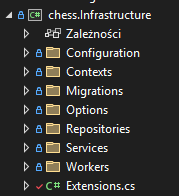
\includegraphics[width=\linewidth]{images/struktura_back_infrastructure.png} 
\end{minipage}
\vspace{0.5cm}

\noindent \textbf{Warstwa logiki biznesowej}\\
Moduł \textbf{.Core} stanowi serce aplikacji i zawiera jej logikę biznesową oraz kluczowe modele domenowe. Jest to najbardziej niezależna warstwa, która nie zna szczegółów implementacyjnych zewnętrznych warstw. Wszystkie zależności są odwrócone – moduł Core definiuje interfejsy, które są implementowane przez warstwę infrastrukturalną, co pozwala na łatwą wymianę technologii bez wpływu na rdzeń aplikacji.

\vspace{0.5cm}
\begin{minipage}[t]{0.45\textwidth}
    \vspace{0pt}
    \centering
    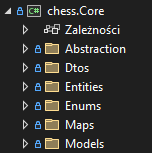
\includegraphics[width=\linewidth]{images/struktura_back_core.png} 
\end{minipage}
\hfill
\begin{minipage}[t]{0.45\textwidth}
    \vspace{0pt}
    \raggedright
    Warstwa domenowa stanowi fundament aplikacji, zawierając kluczowe definicje i logikę biznesową. W folderze Entities znajdują się główne encje, odpowiadające za przechowywanie danych. Enums zawiera wyliczenia, które definiują stałe wartości. W Abstractions znajdują się abstrakcyjne klasy, które są dziedziczone przez podobne encje. Dtos zawiera obiekty transferu danych zwracane przez zapytania, które są dzielone pomiędzy różnymi zapytaniami. Models przechowuje wspólne modele używane przez różne procesy. W Maps znajduje się logika mapowania danych w postaci słowników, który definiuje operacje pobierania i aktualizowania wartości w encjach.
\end{minipage}

\newpage

\noindent \textbf{Warstwa wspólna}\\
Moduł \textbf{.Shared} zawiera wspólne komponenty i funkcjonalności, które są wykorzystywane przez inne warstwy aplikacji. Celem tej warstwy jest centralizacja użytecznych elementów, które nie są specyficzne dla jednej warstwy, a są wykorzystywane przez różne części systemu. Dzięki temu wspólne elementy, takie jak wyjątki, middleware oraz konfiguracje, są łatwo dostępne, a zarządzanie nimi jest uproszczone. Warstwa ta pełni rolę wspierającą, zapewniając rozwiązania, które mogą być współdzielone przez inne warstwy aplikacji, co zwiększa spójność i ułatwia konserwację systemu.

\begin{minipage}[t]{0.45\textwidth}
    \vspace{0pt}
    \raggedright
    Warstwa wspólna Shared zawiera wspólne komponenty, które są wykorzystywane przez inne warstwy aplikacji. Folder Exceptions przechowuje wyjątki, które pozwalają na precyzyjne zarządzanie błędami w systemie. Middleware zawiera komponenty pośredniczące, które przechwytują i obsługują błędy HTTP, zapewniając odpowiednie kody statusu oraz komunikaty w odpowiedzi. W folderze Options znajdują się rozszerzenia umożliwiające łatwe pobieranie konfiguracji z pliku appsettings, co zapewnia centralne zarządzanie ustawieniami aplikacji.
\end{minipage}
\hfill
\begin{minipage}[t]{0.45\textwidth}
    \vspace{0pt}
    \centering
    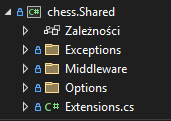
\includegraphics[width=\linewidth]{images/struktura_back_shared.png} 
\end{minipage}
\vspace{0.5cm}

\noindent
Główne moduły projektu, są zintegrowane w aplikacji za pomocą specjalnych klas rozszerzeń (\textbf{Extensions}). Te metody rozszerzeń zapewniają wstrzyknięcie zależności oraz konfigurację wymaganych usług w projekcie, co pozwala na spójne i centralne zarządzanie konfiguracją każdego modułu. Każda z metod, wstrzykuje zależności specyficzne dla danej warstwy, po czym w głównej klasie \textbf{Program} następuje ich rejestracja. Plik ten odpowiada również za rejestracje niestandardowych komponentów, odpowiadają za dodanie specyficznych funkcji.

\vspace{0.5cm}
\begin{figure}[h!]
    \centering
    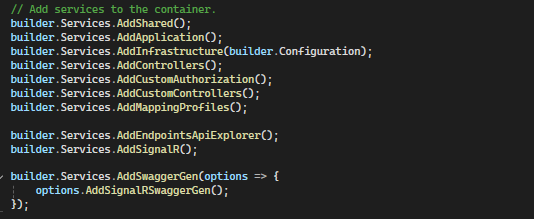
\includegraphics[width=0.7\textwidth]{images/ex_add_services.png}
    \caption{Fragment kodu: Przykład rejestracji serwisów w klasie Program.}
\end{figure}
\vspace{0.5cm}

\noindent 
Oprócz głównych modułów projekt zawiera także dwa dodatkowe moduły wspierające procesy testowania aplikacji. Moduły te są integralną częścią projektu, pomagając zapewnić jakość i niezawodność kodu. Poniżej przedstawiono szczegółowy opis oraz strukture solucji testowych.

\newpage

\noindent \textbf{Warstwa testów integracyjnych}\\
Moduł \textbf{.Api.Tests} zawiera testy integracyjne dla kontrolerów API, zapewniając weryfikację poprawności działania interfejsu API w kontekście integracji z innymi komponentami systemu, takimi jak baza danych czy logika aplikacyjna. Testy te sprawdzają, czy odpowiedzi API są zgodne z oczekiwaniami, weryfikując m.in. poprawność danych wejściowych i wyjściowych oraz obsługę błędów. Każdy folder w tym module odpowiada pojedynczemu kontrolerowi API, umożliwiając modularne testowanie poszczególnych elementów aplikacji. Dzięki testom integracyjnym możliwe jest sprawdzenie, czy aplikacja poprawnie reaguje na różnorodne scenariusze i przypadki brzegowe.

\vspace{0.5cm}
\begin{minipage}[t]{0.45\textwidth}
    \vspace{0pt}
    \centering
    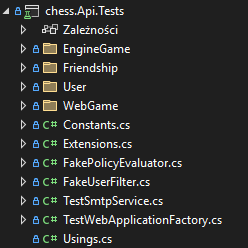
\includegraphics[width=\linewidth]{images/struktura_back_api_tests.png} 
\end{minipage}
\hfill
\begin{minipage}[t]{0.45\textwidth}
    \vspace{0pt}
    \raggedright
    Warstwa ten zawiera testy integracyjne dla kontrolerów API. Każdy folder w tej warstwie odpowiada jednemu kontrolerowi API, umożliwiając modularne testowanie różnych części aplikacji. Testy wykorzystują narzędzia takie jak FluentAssertions i XUnit do tworzenia środowiska testowego. Testy te sprawdzają integrację kontrolera API z bazą danych oraz logiką aplikacyjną, testując poprawne działanie czy obsługę błędów w przypadku niepoprawnych danych wejściowych.
\end{minipage}
\vspace{0.5cm}

\noindent \textbf{Warstwa testów logiki biznesowej}\\
Moduł \textbf{.Core.Tests} zawiera testy jednostkowe dla logiki biznesowej aplikacji. Testy te weryfikują poprawność działania poszczególnych komponentów wewnętrznych systemu, takich jak handled żądań, serwisy, repozytoria oraz inne elementy logiki biznesowej. Dzięki tym testom możliwe jest zapewnienie, że logika aplikacji działa zgodnie z wymaganiami, niezależnie od zewnętrznych zależności. Testy jednostkowe pozwalają na szybsze i łatwiejsze identyfikowanie błędów w samej logice aplikacji, zanim zmiany wpłyną na inne warstwy systemu.

\vspace{0.5cm}
\begin{minipage}[t]{0.45\textwidth}
    \vspace{0pt}
    \raggedright
    Warstwa testów zawiera testy jednostkowe dla logiki biznesowej aplikacji. Testy są podzielone na foldery odpowiadające poszczególnym kontrolerom. Celem tych testów jest weryfikacja poprawności działania komponentów aplikacji, takich jak handlerów żądań, serwisów, czy repozytoriów. Testy skupiają się na sprawdzeniu logiki biznesowej, walidacji danych, oraz obsługi wyjątków, wykorzystując narzędzia takie jak mocki, aby izolować testowane jednostki od zewnętrznych zależności.
\end{minipage}
\hfill
\begin{minipage}[t]{0.45\textwidth}
    \vspace{0pt}
    \centering
    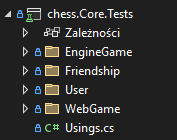
\includegraphics[width=\linewidth]{images/struktura_back_core_tests.png} 
\end{minipage}

\newpage

\subsubsection{REST API}

Interfejsy API są najpopularniejszym sposobem interakcji programów i urządzeń w nowoczesnych technologiach obliczeniowych. API to zestaw reguł opisujących, jak jeden program może się łączyć oraz komunikować z innym. Jak sama nazwa wskazuje, API REST przekazuje na każde żądanie stan każdej transakcji, co daje korzyści związane z opracowaniem, wydajnością i zasobami w porównaniu do innych metod. REST rozwija się w ciągu ponad dwóch dekad i jest bardzo powszechnym podejściem do architektur opartych na usługach i architektur rozproszonych.
\\\\
Zasób jest podstawowym pojęciem dla API REST. Zasób jest obiektem, który ma typ, powiązane dane, relacje z innymi zasobami i zestaw metod, które na nim działają. Jest bardzo podobny do idei obiektów w programowaniu, chociaż zdefiniowanych jest tylko kilka standardowych metod, typowych dla HTTP \textbf{\colorbox{cyan!90}{\textcolor{white}{GET}}}, \textbf{\colorbox{green!90}{\textcolor{white}{POST}}}, \textbf{\colorbox{orange!90}{\textcolor{white}{PUT}}} i \textbf{\colorbox{red!90}{\textcolor{white}{DELETE}}}. Zasoby mogą istnieć same lub w zbiorach, które same są zasobami.
\\\\
W nowoczesnej informatyce wspólnym modelem - również podstawowym dla API REST - jest klient-serwer, gdzie klient, który potrzebuje zasobu, identyfikuje się i komunikuje z serwerem, który może go dostarczyć. W ten sposób zarządzany jest praktycznie cały ruch w chmurze, gdyż oferuje maksymalną elastyczność licznym klientom i pozwala na dostęp do licznych serwerów. Zasada ta sprawdza się również w przypadku tzw. architektur „bezserwerowych", w których miejsce serwera znanego klientowi zajmuje broker usług.
\\\\

\noindent \textbf{Kontrolery API} \\
W systemie REST API zdefiniowane zostały cztery główne kontrolery, które odpowiadają za obsługę zapytań związanych z różnymi zasobami w aplikacji:

\begin{itemize}
    \item \textbf{UserController} - Odpowiada za zapytania związane z użytkownikami, takie jak rejestracja, logowanie, aktualizacja danych czy zarządzanie profilem.
    \item \textbf{FriendshipController} - Obsługuje zapytania dotyczące znajomości między użytkownikami, takie jak zapraszanie do znajomości, akceptowanie lub odrzucanie zaproszeń oraz zarządzanie relacjami.
    \item \textbf{WebGameController} - Zajmuje się zapytaniami dotyczącymi gier online pomiędzy użytkownikami, pozwalając na tworzenie, aktualizowanie i zarządzanie grami.
    \item \textbf{EngineGameController} - Odpowiada za zapytania związane z grami offline, które są rozgrywane z wykorzystaniem silnika szachowego, w tym rozpoczęcie gry, wykonywanie ruchów czy zmiana poziomu trudności.
\end{itemize}

\noindent
Na następnej stronie opisano szczegółowo poszczególne endpointy dostępne w ramach każdego z kontrolerów.

\newpage

\textbf{Endpointy kontrolera UserController}
\begin{itemize} 
    \item \textbf{\colorbox{green!90}{\textcolor{white}{POST}} /api/user/sign-up} \\
    Rejestruje użytkownika i wysyła kod weryfikacyjny e-mailem. 
    \item \textbf{\colorbox{green!90}{\textcolor{white}{POST}} /api/user/sign-in} \\
    Loguje użytkownika i generuje token JWT. 
    \item \textbf{\colorbox{green!90}{\textcolor{white}{POST}} /api/user/regenerate-code} \\
    Generuje nowy kod weryfikacyjny, usuwając stary, dla użytkowników, którzy jeszcze nie zweryfikowali swojego konta. 
    \item \textbf{\colorbox{orange!90}{\textcolor{white}{PUT}} /api/user/verify-email} \\
    Weryfikuje adres e-mail użytkownika za pomocą dostarczonego kodu. 
    \item \textbf{\colorbox{orange!90}{\textcolor{white}{PUT}} /api/user/send-password-code} \\
    Wysyła kod weryfikacyjny do odzyskania hasła. 
    \item \textbf{\colorbox{orange!90}{\textcolor{white}{PUT}} /api/user/reset-password} \\
    Resetuje hasło użytkownika po podaniu kodu weryfikacyjnego. 
    \item \textbf{\colorbox{orange!90}{\textcolor{white}{PUT}} /api/user/change-password} \\
    Zmienia hasło użytkownika, dostępne tylko dla użytkowników, którzy są zalogowani i zweryfikowani. 
    \item \textbf{\colorbox{orange!90}{\textcolor{white}{PUT}} /api/user/profile} \\
    Aktualizuje dane profilu użytkownika. 
    \item \textbf{\colorbox{orange!90}{\textcolor{white}{PUT}} /api/user/data} \\
    Zmienia dane użytkownika, takie jak imię, nazwisko itp. 
    \item \textbf{\colorbox{orange!90}{\textcolor{white}{PUT}} /api/user/settings} \\
    Zmienia ustawienia użytkownika, np. preferencje konta. 
    \item \textbf{\colorbox{cyan!90}{\textcolor{white}{GET}} /api/user} \\
    Pobiera podstawowe informacje o użytkowniku. 
    \item \textbf{\colorbox{cyan!90}{\textcolor{white}{GET}} /api/user/full} \\
    Pobiera pełne informacje o użytkowniku, takie jak historia, rankingi, szczegóły profilu. 
    \item \textbf{\colorbox{cyan!90}{\textcolor{white}{GET}} /api/user/{userId}/other} \\
    Pobiera informacje o innym użytkowniku, np. publiczne dane profilu. 
    \item \textbf{\colorbox{cyan!90}{\textcolor{white}{GET}} /api/user/elo} \\
    Pobiera informacje o rankingu Elo użytkownika. 
    \item \textbf{\colorbox{cyan!90}{\textcolor{white}{GET}} /api/user/is-verified} \\
    Sprawdza, czy adres e-mail użytkownika jest zweryfikowany. 
    \item \textbf{\colorbox{cyan!90}{\textcolor{white}{GET}} /api/user/by-email} \\
    Pobiera dane użytkownika na podstawie podanego adresu e-mail. 
    \item \textbf{\colorbox{cyan!90}{\textcolor{white}{GET}} /api/user/configuration} \\
    Pobiera konfigurację rejestracji użytkownika. 
    \item \textbf{\colorbox{cyan!90}{\textcolor{white}{GET}} /api/user/ranking} \\
    Pobiera globalny ranking użytkowników. 
\end{itemize}

\newpage

\textbf{Endpointy kontrolera FriendshipController}
\begin{itemize} 
    \item \textbf{\colorbox{green!90}{\textcolor{white}{POST}} /api/friendship/invite} \\
    Tworzy zaproszenie do znajomości z oczekującym statusem. 
    \item \textbf{\colorbox{green!90}{\textcolor{white}{POST}} /api/friendship/block} \\
    Tworzy zaproszenie do znajomości z odrzuconym statusem. 
    \item \textbf{\colorbox{orange!90}{\textcolor{white}{PUT}} /api/friendship/{friendshipId}/respond} \\
    Zmienia status oczekującej znajomości (akceptacja lub odrzucenie zaproszenia). 
    \item \textbf{\colorbox{cyan!90}{\textcolor{white}{GET}} /api/friendship/all-by-status} \\
    Pobiera wszystkich użytkowników z określonym statusem relacji (znajomi, oczekujący, zablokowani). 
    \item \textbf{\colorbox{cyan!90}{\textcolor{white}{GET}} /api/friendship/all-non} \\
    Pobiera wszystkich użytkowników, którzy nie są w relacji z użytkownikiem. 
    \item \textbf{\colorbox{cyan!90}{\textcolor{white}{GET}} /api/friendship/{friendshipId}/profile} \\
    Pobiera profil znajomego na podstawie identyfikatora znajomości. 
    \item \textbf{\colorbox{cyan!90}{\textcolor{white}{GET}} /api/friendship/ranking} \\
    Pobiera ranking użytkowników wśród znajomych na podstawie wybranego modelu. 
    \item \textbf{\colorbox{cyan!90}{\textcolor{white}{GET}} /api/friendship/{friendshipId}/games} \\
    Pobiera listę gier rozegranych w ramach znajomości. 
    \item \textbf{\colorbox{red!90}{\textcolor{white}{DELETE}} /api/friendship/{friendshipId}} \\
    Usuwa znajomość lub odblokowuje użytkownika (w zależności od istniejącej relacji). 
\end{itemize}

\newpage

\textbf{Endpointy kontrolera WebGameController}
\begin{itemize} 
    \item \textbf{\colorbox{green!90}{\textcolor{white}{POST}} /api/webgame/search} \\
    Inicjuje poszukiwanie gry online, tworzy gracza i ustawia czas gry, jeśli nie istnieje. 
    \item \textbf{\colorbox{green!90}{\textcolor{white}{POST}} /api/webgame/private} \\
    Tworzy prywatną grę i zwraca jej identyfikator. 
    \item \textbf{\colorbox{green!90}{\textcolor{white}{POST}} /api/webgame/email} \\
    Tworzy prywatną grę przez podanie adresu e-mail przeciwnika, zwraca identyfikator gry. 
    \item \textbf{\colorbox{green!90}{\textcolor{white}{POST}} /api/webgame/link} \\
    Tworzy prywatną grę z linkiem, który umożliwia dostęp do gry, zwraca identyfikator gry. 
    \item \textbf{\colorbox{cyan!90}{\textcolor{white}{GET}} /api/webgame/is-in-game} \\
    Sprawdza, czy gracz jest już w grze. 
    \item \textbf{\colorbox{cyan!90}{\textcolor{white}{GET}} /api/webgame/{gameId}/update-required} \\
    Sprawdza, czy wymagana jest aktualizacja stanu gry dla gry stworzonej za pomocą linku. 
    \item \textbf{\colorbox{cyan!90}{\textcolor{white}{GET}} /api/webgame/{gameId}} \\
    Pobiera pełne dane gry na podstawie identyfikatora ID. 
    \item \textbf{\colorbox{cyan!90}{\textcolor{white}{GET}} /api/webgame/{gameId}/player} \\
    Pobiera dane gracza w danej grze. 
    \item \textbf{\colorbox{cyan!90}{\textcolor{white}{GET}} /api/webgame/{gameId}/time} \\
    Pobiera czas pozostały dla gracza w danej grze. 
    \item \textbf{\colorbox{cyan!90}{\textcolor{white}{GET}} /api/webgame/{gameId}/opponent} \\
    Pobiera dane przeciwnika z zakończonej gry. 
    \item \textbf{\colorbox{cyan!90}{\textcolor{white}{GET}} /api/webgame/{gameId}/timing} \\
    Pobiera konfigurację czasu gry (timing) dla danej gry. 
    \item \textbf{\colorbox{cyan!90}{\textcolor{white}{GET}} /api/webgame/all-ongoing} \\
    Pobiera wszystkie aktywne gry dla użytkownika. 
    \item \textbf{\colorbox{cyan!90}{\textcolor{white}{GET}} /api/webgame/all-finished} \\
    Pobiera wszystkie zakończone gry dla użytkownika. 
    \item \textbf{\colorbox{cyan!90}{\textcolor{white}{GET}} /api/webgame/type-history} \\
    Pobiera historię gier dla wybranego typu czasu gry. 
    \item \textbf{\colorbox{cyan!90}{\textcolor{white}{GET}} /api/webgame/invitations} \\
    Pobiera wszystkie zaproszenia do gier, które zostały jeszcze nieodebrane. 
    \item \textbf{\colorbox{cyan!90}{\textcolor{white}{GET}} /api/webgame/{gameId}/messages} \\
    Pobiera wszystkie wiadomości z danej gry. 
    \item \textbf{\colorbox{cyan!90}{\textcolor{white}{GET}} /api/webgame/stats} \\
    Pobiera statystyki wszystkich gier rozegranych przez użytkownika. 
    \item \textbf{\colorbox{red!90}{\textcolor{white}{DELETE}} /api/webgame/abort} \\
    Anuluje poszukiwanie gry online. 
    \item \textbf{\colorbox{red!90}{\textcolor{white}{DELETE}} /api/webgame/{gameId}/cancel} \\
    Anuluje prywatną grę. Usuwa graczy. 
\end{itemize}

\newpage

\textbf{Endpointy kontrolera EngineGameController}
\begin{itemize} 
    \item \textbf{\colorbox{green!90}{\textcolor{white}{POST}} /api/enginegame/start}\\
    Rozpoczyna nową grę z silnikiem szachowym. 
    \item \textbf{\colorbox{green!90}{\textcolor{white}{POST}} /api/enginegame/{gameId}/make-move}\\
    Wykonuje ruch w grze, wykonany przez gracza lub silnik.
    \item \textbf{\colorbox{orange!90}{\textcolor{white}{PUT}} /api/enginegame/{gameId}/end-game}\\
    Kończy grę z silnikiem szachowym. 
    \item \textbf{\colorbox{orange!90}{\textcolor{white}{PUT}} /api/enginegame/{gameId}/change-engine}\\
    Zmienia poziom trudności silnika szachowego. 
    \item \textbf{\colorbox{orange!90}{\textcolor{white}{PUT}} /api/enginegame/{gameId}/undo-move}\\
    Cofnięcie ostatniego wykonanego ruchu. 
    \item \textbf{\colorbox{orange!90}{\textcolor{white}{PUT}} /api/enginegame/update-settings}\\
    Aktualizuje ustawienia związane z grami z silnikiem szachowym. 
    \item \textbf{\colorbox{cyan!90}{\textcolor{white}{GET}} /api/enginegame/{gameId}}\\
    Pobiera wszystkie dane dotyczące gry z silnikiem szachowym.
    \item \textbf{\colorbox{cyan!90}{\textcolor{white}{GET}} /api/enginegame/{gameId}/winner}\\
    Pobiera zwycięzcę gry z silnikiem szachowym. 
    \item \textbf{\colorbox{cyan!90}{\textcolor{white}{GET}} /api/enginegame/{gameId}/engine-move}\\
    Pobiera ruch wykonany przez silnik w grze. 
    \item \textbf{\colorbox{cyan!90}{\textcolor{white}{GET}} /api/enginegame/{gameId}/all-messages}\\
    Pobiera wszystkie wiadomości związane z aktualną grą z silnikiem. 
    \item \textbf{\colorbox{cyan!90}{\textcolor{white}{GET}} /api/enginegame/all-games}\\
    Pobiera wszystkie gry z silnikiem szachowym. 
\end{itemize}

\newpage

\noindent \textbf{Dokumentowanie API przy użyciu Swaggera}\\
Aby lepiej zilustrować strukturę i funkcjonalność REST API, poniżej przedstawiono przykład endpointów wygenerowanych automatycznie za pomocą biblioteki Swagger. Swagger umożliwia dokumentowanie API w sposób przejrzysty i interaktywny, co znacznie ułatwia zarówno tworzenie, jak i korzystanie z interfejsów API przez programistów.

\begin{figure}[h!]
    \centering
    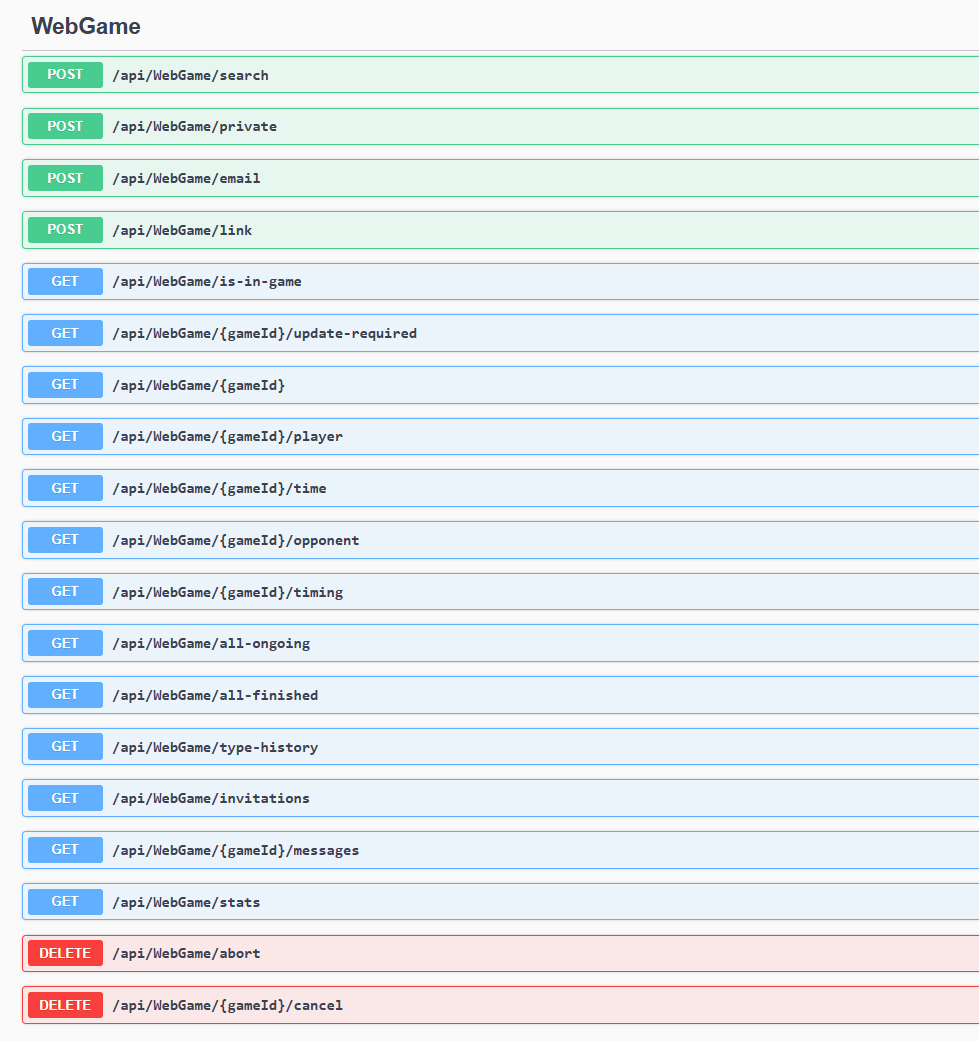
\includegraphics[width=1\textwidth]{images/swagger_api.png}
    \caption{Przykład endpointów wygenerowanych za pomocą biblioteki Swagger.}
\end{figure}

\newpage

\subsubsection{SignalR}
SignalR to biblioteka opracowana przez Microsoft, która umożliwia dodanie funkcji komunikacji w czasie rzeczywistym do aplikacji. Jest szczególnie przydatna w scenariuszach wymagających natychmiastowego przesyłania danych między serwerem a klientem, takich jak czaty, powiadomienia, aktualizacje w czasie rzeczywistym w aplikacjach finansowych, gier czy dashboardach.
\\\\
Główną zaletą SignalR jest ukrycie złożoności związanej z obsługą komunikacji w czasie rzeczywistym. Biblioteka automatycznie wybiera najlepszy dostępny mechanizm komunikacji w zależności od środowiska aplikacji, w tym:

\begin{itemize}
    \item \textbf{WebSockets} – preferowana metoda, jeśli jest obsługiwana przez przeglądarkę i serwer, zapewnia pełny duplex komunikacji.
    \item \textbf{Server-Sent Events} – alternatywa dla WebSockets, jednokierunkowa komunikacja serwera z klientem.
    \item \textbf{Long Polling} – metoda zastępcza, w której klient wysyła powtarzające się zapytania do serwera, oczekując odpowiedzi.
\end{itemize}

\noindent
SignalR opiera się na modelu hubów, które służą jako centralny punkt komunikacji. Klient i serwer mogą wysyłać wiadomości do huba, który z kolei przesyła je do odpowiednich odbiorców. 
\\\\
Podstawowe kroki działania SignalR to:

\begin{itemize}
    \item Klient nawiązuje połączenie z serwerem za pomocą huba.
    \item Hub zarządza komunikacją, przekazując wiadomości między serwerem a klientami.
    \item Klienci mogą nasłuchiwać na określone metody w hubie i reagować na otrzymane dane.
    \item Serwer może w dowolnym momencie wysyłać wiadomości do połączonych klientów.
\end{itemize}

\noindent
SignalR zapewnia wysoki poziom abstrakcji, dzięki czemu programista nie musi martwić się o szczegóły implementacyjne różnych protokołów komunikacji, co czyni go bardzo elastycznym i wydajnym rozwiązaniem.
\\\\
W aplikacji utworzono jedną klasę huba, która odpowiada za obsługę gier online. Klasa ta centralizuje komunikację między klientami a serwerem, umożliwiając natychmiastowe przesyłanie danych, takich jak ruchy w grze czy informacje o stanie gry.
\\\\
Dodatkowo stworzono interfejs, który definiuje metody wywoływane przez odpowiednich klientów. Interfejs ten pełni rolę kontraktu, gwarantując, że klienci będą mieli dostęp do spójnych metod obsługi gier online. Dzięki temu różne typy klientów mogą w prosty sposób integrować się z hubem i korzystać z jego funkcji, takich jak wysyłanie ruchu, odbieranie powiadomień czy synchronizacja danych w czasie rzeczywistym.
\\\\
Na następnej stronie przedstawiono szczegółowy opis metod dostępnych w ramach interfejsu SignalR, z podziałem na typy zapytań.

\newpage

\begin{itemize}
    \setlength\itemsep{0.1cm}
    \item \textbf{\colorbox{green!90}{\textcolor{white}{POST}} /game-hub/add-self-notification}\\
    Dodaje użytkownika do grupy powiadomień, umożliwiając odbieranie powiadomień.
    \item \textbf{\colorbox{green!90}{\textcolor{white}{POST}} /game-hub/add-player}\\
    Dodaje użytkownika do grupy gry i wysyła żądanie weryfikacji dostępu.
    \item \textbf{\colorbox{green!90}{\textcolor{white}{POST}} /game-hub/player-joined}\\
    Dodaje użytkownika do kolejki gry / rozpoczyna gry online.
    \item \textbf{\colorbox{green!90}{\textcolor{white}{POST}} /game-hub/rematch}\\
    Tworzy nową grę dla dwóch tych samych graczy, którzy już rozegrali jedną partię.
    \item \textbf{\colorbox{green!90}{\textcolor{white}{POST}} /game-hub/make-move}\\
    Wykonuje ruch w grze i aktualizuje jej stan.
    \item \textbf{\colorbox{green!90}{\textcolor{white}{POST}} /game-hub/send-player-message}\\
    Wysyła wiadomość graczowi w ramach bieżącej gry.
    \item \textbf{\colorbox{green!90}{\textcolor{white}{POST}} /game-hub/send-game-message}\\
    Wysyła wiadomość w grze dla wszystkich graczy.
    \item \textbf{\colorbox{green!90}{\textcolor{white}{POST}} /game-hub/send-draw-message}\\
    Wysyła propozycję remisu.
    \item \textbf{\colorbox{orange!90}{\textcolor{white}{PUT}} /game-hub/end-game}\\
    Kończy grę i aktualizuje jej parametry końcowe.
    \item \textbf{\colorbox{orange!90}{\textcolor{white}{PUT}} /game-hub/accept-rematch}\\
    Akceptuje propozycję rewanżu, powiadamia obu graczy i rozpoczyna grę.
    \item \textbf{\colorbox{orange!90}{\textcolor{white}{PUT}} /game-hub/accept-invitation}\\
    Akceptuje zaproszenie do gry, powiadamia graczy i rozpoczyna grę.
    \item \textbf{\colorbox{orange!90}{\textcolor{white}{PUT}} /game-hub/update-private-game}\\
    Aktualizuje prywatną grę utworzoną przez link.
    \item \textbf{\colorbox{orange!90}{\textcolor{white}{PUT}} /game-hub/typing-status}\\
    Aktualizuje status pisania użytkownika.
    \item \textbf{\colorbox{cyan!90}{\textcolor{white}{GET}} /game-hub/get-winner}\\
    Pobiera dane zwycięzcy gry.
    \item \textbf{\colorbox{cyan!90}{\textcolor{white}{GET}} /game-hub/notify-user}\\
    Dostarcza dane niezbędne zaproszonemu użytkownikowi do zaakceptowania gry.
    \item \textbf{\colorbox{red!90}{\textcolor{white}{DELETE}} /game-hub/player-leaved}\\
    Usuwa gracza z kolejki gry.
    \item \textbf{\colorbox{red!90}{\textcolor{white}{DELETE}} /game-hub/leave-game}\\
    Usuwa użytkownika z połączenia z grą.
    \item \textbf{\colorbox{red!90}{\textcolor{white}{DELETE}} /game-hub/decline-invitation}\\
    Odrzuca zaproszenie do gry i powiadamia zapraszającego.
    \item \textbf{\colorbox{red!90}{\textcolor{white}{DELETE}} /game-hub/remove-draw}\\
    Odrzuca propozycję remisu.
    \item \textbf{\colorbox{red!90}{\textcolor{white}{DELETE}} /game-hub/cancel-rematch}\\
    Anuluje ofertę rewanżu w grze.
\end{itemize}

\newpage

\noindent \textbf{Metody po stronie klienta}
Interfejs \textcolor{teal}{\textbf{IGameHub}} definiuje zestaw metod, które są dostępne do wywołania przez klienta, po otrzymaniu powiadomienia z serwera. Poniżej wypisano metody zadeklarowane w interfejsie:

\begin{itemize}
    \item \textbf{GamesChanged} \\
    Metoda ta służy do powiadamiania grupy w kolejce o utworzonych grach. Zwykle wywoływana, gdy nowe gry zostały stworzone, aby powiadomić użytkowników oczekujących w kolejce.
    \item \textbf{GameUpdated} \\
    Ta metoda informuje wszystkich użytkowników w grupie gry, że wykonano ruch w grze. Powiadomienie jest wysyłane do wszystkich osób biorących udział w danej grze.
    \item \textbf{GameEnded} \\
    Metoda służy do powiadamiania użytkowników o zakończeniu gry. Używana po zakończeniu gry, aby powiadomić uczestników, że gra dobiegła końca.
    \item \textbf{InvitedToGame} \\
    Metoda umożliwia wysłanie zaproszenia do gry. Powiadamia zaproszoną osobę o grze, która została dla niej utworzona. Parametr \texttt{dto} zawiera szczegóły dotyczące zaproszenia.
    \item \textbf{GameAccepted} \\
    Ta metoda informuje użytkowników, że zaproszenie do gry zostało zaakceptowane. Obie strony są powiadamiane o rozpoczęciu gry.
    \item \textbf{MessagesUpdated} \\
    Metoda ta powiadamia użytkowników o nowych wiadomościach wysłanych w grze. Jest wywoływana, gdy jeden z uczestników gry wyśle nową wiadomość do drugiego gracza.
    \item \textbf{InvitationDeclined} \\
    Metoda używana do powiadamiania o odrzuceniu zaproszenia do gry. Powiadamia osobę, która wysłała zaproszenie, że zaproszona osoba je odrzuciła.
    \item \textbf{TypingStatus} \\
    Metoda umożliwia powiadomienie o stanie pisania w grze. Parametr \texttt{IsTyping} określa, czy użytkownik aktualnie pisze wiadomość, co służy do pokazania animacji pisania w interfejsie użytkownika.
    \item \textbf{RematchRequested} \\
    Metoda ta służy do powiadamiania graczy o ofercie rewanżu. Powiadamia użytkowników, że druga osoba zaproponowała rematch (powtórkę gry). Zwraca one dane dotyczące rematchu.
    \item \textbf{RematchCanceled} \\
    Ta metoda informuje użytkowników, że oferta rewanżu została anulowana. Jest używana, gdy jedna ze stron postanowi wycofać swoją ofertę rematchu.
    \item \textbf{GetWinner} \\
    Metoda do uzyskania informacji o zwycięzcy zakończonej gry. Parametr \texttt{dto} zawiera dane dotyczące wyniku gry, w tym informacje o wygranej stronie.
\end{itemize}


\newpage

\subsubsection{Komunikacja z silnikiem}

\begin{minipage}[t]{0.2\textwidth} 
    \vspace{0pt} 
    \centering
    
\includegraphics[width=\linewidth]{images/stockfish_logo.png} 
\end{minipage} 
\hfill 
\begin{minipage}[t]{0.7\textwidth} 
    \vspace{0pt} 
    \raggedright 
    Silnik szachowy Stockfish jest jednym z najpotężniejszych i najczęściej używanych silników szachowych na świecie. Jest to oprogramowanie typu open-source, które zostało stworzone, aby oferować najwyższą możliwą siłę obliczeniową w grach szachowych. Stockfish jest napisany w języku C++ i jest dostępny na wiele platform, w tym na systemy Windows, Linux, macOS, a także urządzenia mobilne.
\end{minipage} 
\vspace{1cm}

Stockfish jest oparty na algorytmie minimax, który jest popularnym podejściem w sztucznej inteligencji do podejmowania decyzji w grach dwuosobowych, takich jak szachy. Algorytm ten stara się ocenić każde możliwe posunięcie, wybierając to, które zapewnia najlepszy wynik, bazując na analizie możliwych przyszłych ruchów. Używa on także heurystyk oraz analizy pozycyjnej, aby ocenić siłę danej pozycji na szachownicy. Co więcej, Stockfish jest w stanie analizować partie z dużą prędkością, co czyni go idealnym narzędziem do analizy gier na różnych poziomach zaawansowania.
\\\\
Jednym z kluczowych aspektów Stockfish jest jego zdolność do pracy w ramach protokołu UCI (Universal Chess Interface). UCI jest standardem, który umożliwia komunikację między silnikiem szachowym a różnymi interfejsami graficznymi (GUI), pozwalając na łatwą integrację z aplikacjami szachowymi. Dzięki temu użytkownicy mogą korzystać z graficznych interfejsów, takich jak Arena, Fritz czy lichess, aby bezpośrednio połączyć się z silnikiem Stockfish, wybierając odpowiednią wersję i parametry.
\\\\
Silnik Stockfish jest również wykorzystywany do tworzenia testów i analiz w wielu aplikacjach szachowych, zarówno komercyjnych, jak i akademickich. Dzięki swojej mocy obliczeniowej, dokładności i dostępności, Stockfish stał się nieocenionym narzędziem w wielu dziedzinach związanych z szachami, od profesjonalnych gier po badania naukowe.
\\\\
W kontekście komunikacji z silnikiem Stockfish, aplikacja korzysta z interfejsu UCI, wysyłając zapytania w postaci komend tekstowych do silnika, który następnie odpowiada, udzielając wskazówek dotyczących najlepszych posunięć, oceniając pozycje lub generując pełną analizę partii. UCI zapewnia, że aplikacja może zarządzać różnymi funkcjami silnika, jak generowanie ruchów, ustawienie poziomu trudności czy analiza pozycji na szachownicy.
\\\\
Aby uzyskać szczegółowe informacje na temat silnika Stockfish, jego funkcji oraz dokumentacji, można zapoznać się z jego repozytorium na GitHubie: 

\begin{center}
    \textbf{\href{https://github.com/official-stockfish/Stockfish}{https://github.com/official-stockfish/Stockfish}}
\end{center}

\newpage

\noindent
Komunikacja z silnikiem szachowym jest kluczowym elementem w budowie aplikacji, która ma na celu interakcję z popularnymi silnikami szachowymi, takimi jak Stockfish. W przedstawionym przykładzie wykorzystano klasę \textbf{EngineService}, która zapewnia funkcjonalność umożliwiającą komunikację z procesem silnika.
\\\\
Sam silnik działa jako aplikacja uruchamiana w tle na serwerze, co pozwala na obsługę wielu równoczesnych zapytań i zapewnia wydajną współpracę z innymi komponentami aplikacji.
\\\\
Klasa ta implementuje interfejs \texttt{IEngineService}, co zapewnia jednolitość i ułatwia integrację z innymi komponentami aplikacji. W konstruktorze tej klasy tworzony jest obiekt typu \textbf{Process}, który uruchamia silnik szachowy. Proces jest konfigurowany tak, aby nie tworzył okna i umożliwiał przesyłanie danych zarówno do silnika - poprzez standardowe wejście, jak i z silnika - poprzez standardowe wyjście.

\begin{itemize} 
    \item \textbf{Startowanie procesu silnika:} W konstruktorze klasy, obiekt typu \textbf{Process} jest konfigurowany za pomocą klasy \textbf{ProcessStartInfo}. Ustawienia te zapewniają, że silnik będzie działał w tle bez interakcji z interfejsem użytkownika, a komunikacja będzie odbywała się za pomocą strumieni wejścia i wyjścia. 
    \item \textbf{Wysyłanie komend do silnika:} Metoda \textbf{SendCommand} pozwala na wysyłanie komend do silnika. Komendy są przesyłane do standardowego wejścia silnika, a następnie natychmiastowo zapisywane do strumienia wyjściowego. 
    \item \textbf{Odczytywanie wyników:} Metoda \textbf{ReadOutput} służy do odczytywania danych wyjściowych z silnika. Wykorzystuje ona strumień wyjściowy, by zbierać linie tekstu, które są następnie przechowywane w liście. Proces odczytu jest ograniczony czasowo, co zapobiega zablokowaniu aplikacji w przypadku długotrwałych odpowiedzi silnika. 
    \item \textbf{Zamykanie procesu:} Metoda \textbf{Close} wysyła do silnika komendę "quit", a następnie zamyka proces, kończąc w ten sposób interakcję z silnikiem. 
\end{itemize}

\noindent
Dzięki takiej implementacji, aplikacja może komunikować się z silnikiem szachowym w sposób asynchroniczny i kontrolować przebieg gry w czasie rzeczywistym, co jest fundamentalne dla prawidłowego funkcjonowania aplikacji.
\\\\

\noindent \textbf{Wykorzystanie serwisu}\\
Implementacja interesu serwisu \texttt{IEngineService} jest wykorzystywany w jednym z handlerów, służącym do zarządzania interakcją z silnikiem szachowym, który oblicza najlepszy ruch w grze na podstawie aktualnej pozycji. Handler ten pełni rolę pośrednika pomiędzy aplikacją a silnikiem, umożliwiając pobieranie ruchów zaproponowanych przez silnik.
\\\\
Na następnej stronie zamieszczono enumerację, która ilustruje krok po kroku, jak działa wspomniany handler i w jaki sposób korzysta on z serwisu.

\newpage

\begin{enumerate}
    \item \textbf{Inicjalizacja serwisu}\\
    W konstruktorze handlera przyjmowane są zależności. Dzięki temu handler ma dostęp do metod serwisu, takich jak SendCommand i ReadOutput, które są kluczowe do interakcji z silnikiem.

    \item \textbf{Przygotowanie do obliczeń}\\
    Po pobraniu gry na podstawie identyfikatora (ID) i walidacji dostępu użytkownika, handler tworzy pełną wersję pozycji szachowej w formacie FEN. Jest standardowy format, który reprezentuje aktualną pozycję na szachownicy. Ten pełny zapis pozycji jest następnie przesyłany do silnika szachowego za pomocą metody \texttt{\textbf{SendCommand}}.

    \item \textbf{Wykonanie obliczeń przez silnik}\\
    Kiedy silnik otrzyma polecenie z pełnym zapisem FEN, handler wysyła kolejną komendę do silnika za pomocą SendCommand, prosząc o wykonanie ruchu na określoną głębokość analizy na podstawie poziomu trudności ustawionego w grze.

    \begin{figure}[h!]
        \centering
        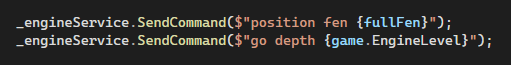
\includegraphics[width=0.8\textwidth]{images/ex_send_command.png}
        \caption{Fragment kodu - przesył zapytania do silnika.}
    \end{figure}

    Serwis \texttt{IEngineService} przesyła tę komendę do silnika, który następnie analizuje pozycję i oblicza najlepszy możliwy ruch.

    \item \textbf{Odczyt odpowiedzi od silnika}\\
    Po wysłaniu komendy, handler oczekuje na odpowiedź od silnika. Metoda \texttt{\textbf{ReadOutput}} serwisu jest używana do odczytywania odpowiedzi, która zawiera najlepszy ruch (komenda bestmove). Odpowiedź ta jest przetwarzana w pętli, aż silnik zwróci ruch lub upłynie czas oczekiwania.
    
    \begin{figure}[h!]
        \centering
        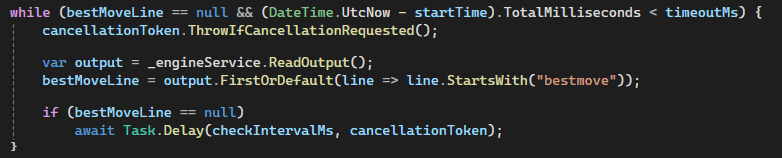
\includegraphics[width=0.8\textwidth]{images/ex_read_output.png}
        \caption{Fragment kodu - wczytywanie odpowiedzi o najlepszym ruchu.}
    \end{figure}

    W przypadku, gdy ruch jest dostępny, jest on wyodrębniany z odpowiedzi i zapisywany.

    \item \textbf{Przetwarzanie najlepszego ruchu}\\
    Po uzyskaniu najlepszego ruchu z silnika, handler konstruuje nową wersję FEN, która reprezentuje pozycję po wykonaniu ruchu. Następnie wysyła kolejne komendy do silnika, aby zaktualizować pozycję w silniku i zwrócić nowe dane, w tym zapis pozycji po ruchu.

    \item \textbf{Zakończenie interakcji}\\
    o zakończeniu obliczeń i uzyskaniu wyników, serwis jest zamykany za pomocą metody \texttt{\textbf{Close}}. To zapewnia, że proces silnika jest zakończony, a wszystkie zasoby systemowe są odpowiednio zwolnione.
\end{enumerate}

\newpage
\subsubsection{Kluczowe mechanizmy gry}

\noindent \textbf{Tworzenie i dołączanie do gier}\\
Proces tworzenia i dołączania do gier w aplikacji można podzielić na trzy główne typy: gry online z losowym graczem, prywatne gry online oraz gry z komputerem. Każdy z tych typów ma swoją specyficzną logikę, która determinuje sposób, w jaki gracze dołączają do gier oraz jak te są one inicjowane.

\begin{itemize}
    \item \textbf{Gry online z losowym graczem}\\
    W przypadku gier online z losowym graczem, użytkownik rozpoczyna proces poszukiwania gry, co skutkuje utworzeniem rekordu gracza. Gracz ten "trafia" do kolejki oczekujących, gdzie oczekuje na innych graczy. Każde dołączenie nowego gracza do kolejki wywołuje mechanizm, który zbiera wszystkich oczekujących graczy i sprawdza, czy warunki do rozpoczęcia gry zostały spełnione.
    \\
    Sprawdzanie, czy można rozpocząć grę, odbywa się w sposób sekwencyjny, zaczynając od graczy, którzy oczekują najdłużej. Jeżeli warunki zostaną spełnione tj. znaleziono graczowi przeciwnika o zbliżonej punktacji, gra zostaje utworzona. Wówczas gracz i jego przeciwnik, są automatycznie dodawani do gry, rozpoczynając wspólną rozgrywkę.
    
    \item \textbf{Prywatne gry online}\\
    Prywatne gry online różnią się od gier losowych tym, że są one tworzone automatycznie przez jednego z użytkowników, drugi natomiast posiada zaproszenie do wspólnej gry. W tym przypadku gra jest tworzona z góry, a gracze zostają od razu przypisani do tej gry, nie oczekując w kolejce.
    \\
    Prywatne gry mają specyficzną cechę — gracze biorący udział w takich grach są oznaczani jako "prywatni". Tacy gracze nie są uwzględniani w systemie wyszukiwania gier online, co oznacza, że nie będą brać udziału w losowych dobieraniach graczy (zgodnie z opisanym wcześniej mechanizmem dla gier online). W związku z tym, prywatne gry odbywają się wyłącznie pomiędzy zaproszonymi graczami.

    \item \textbf{Gry z komputerem}\\
    W przypadku gier z komputerem, proces jest najbardziej zautomatyzowany. Gra z komputerem jest tworzona automatycznie, a użytkownik jest jedynym graczem w grze. Gra nie wymaga oczekiwania na innych graczy, ponieważ przeciwnikiem użytkownika jest komputer. W tym przypadku tworzony jest tylko jeden gracz reprezentujący użytkownika, który bierze udział w grze przeciwko sztucznej inteligencji (silnikowi).
\end{itemize}

\noindent \textbf{Powiadomienia o zmianach stanu kolejki}\\
Aby zapewnić synchronizację pomiędzy graczami i ich reakcję na zmiany stanu kolejki, aplikacja wykorzystuje technologię SignalR. To narzędzie, które pozwala na natychmiastową synchronizację stanu gry pomiędzy graczami, zapewniając, że każdy gracz jest na bieżąco informowany o tym, czy został dołączony do gry, lub czy otrzymał zaproszenie do prywatnej gry. Dzięki tej bibliotece gracze mogą otrzymywać powiadomienia w czasie rzeczywistym, co umożliwia im płynne przejście do etapu gry bez opóźnień.

\newpage

\noindent \textbf{Punktacja ELO}\\
Punktacja ELO to system oceny umiejętności graczy stosowany w aplikacji do określania ich relatywnej siły gry. Mechanizm ten jest dynamiczny, co oznacza, że po każdej zakończonej grze punkty ELO obu graczy są aktualizowane w zależności od wyniku rozgrywki. Wartość zmiany w punktacji jest obliczana na podstawie różnicy punktów między graczami oraz wyniku gry. System uwzględnia pięć kategorii czasowych rozgrywek: bullet, blitz, rapid, classic oraz daily, z których każda ma osobną punktację. Do obliczenie punktacji rozróżnia się trzy główne przypadki:

\begin{itemize}
    \item \textbf{Wygrana lepszego gracza}\\
    Jeśli zwycięzcą gry jest gracz, który przed rozgrywką miał wyższą punktację ELO niż jego przeciwnik, oznacza to, że wynik był bardziej przewidywalny. W takim przypadku zmiana punktacji dla zwycięzcy oraz przegranego jest stosunkowo niewielka, ponieważ potwierdza ona wcześniejsze przypuszczenia o różnicy w umiejętnościach graczy.

    \[ \text{elo}_{\pm} = \lceil \frac{100}{0.1 \cdot \Delta \text{elo} + 10} \rceil \]

    Gdzie $ \text{elo}_{\pm} $ oznacza punkty dodane / odjęte graczom a $ \Delta \text{elo} $ oznacza różnice w punktacji pomiędzy graczami przez rozpoczęciem gry. Im większa różnica w punktacji ELO między graczami, tym mniejsza zmiana punktów dla zwycięzcy, co odzwierciedla mniejsze znaczenie wygranej dla wyżej punktowanego gracza.
    \item \textbf{Wygrana słabszego gracza}\\
    Jeśli zwycięzcą gry jest gracz z niższą punktacją ELO niż jego przeciwnik, wynik jest bardziej zaskakujący, co prowadzi do większych zmian punktacji. W takim przypadku stosuje się wzór:

    \[ \text{elo}_{\pm} = \lceil 0.1 \cdot \Delta \text{elo} + 10 \rceil \]

    Gdzie $ \text{elo}_{\pm} $ oznacza punkty dodane / odjęte graczom a $ \Delta \text{elo} $ oznacza różnice w punktacji pomiędzy graczami przez rozpoczęciem gry. W tym przypadku, większa różnica punktów ELO działa na korzyść zwycięzcy, co skutkuje znaczącym wzrostem jego punktacji. Analogicznie, przegrany, który był wyżej punktowany, traci więcej punktów, co odzwierciedla większą wagę niespodziewanego wyniku.

    \item \textbf{Przypadek remisu}\\
    Remis jest traktowany jako sytuacja, w której obaj gracze osiągają równy wynik, co skutkuje mniejszą zmianą punktacji niż w przypadku zwycięstwa jednego z graczy. Zmiana punktacji w przypadku remisu zależy również od różnicy punktów między graczami. Stosowany jest wzór:

    \[ \text{elo}_{\pm} = \lceil 0.05 \cdot \Delta \text{elo} \rceil \]

    Gdzie $ \text{elo}_{\pm} $ oznacza punkty dodane / odjęte graczom a $ \Delta \text{elo} $ oznacza różnice w punktacji pomiędzy graczami przez rozpoczęciem gry.     W tym przypadku gracz z wyższą punktacją traci punkty, natomiast gracz z niższą zyskuje je, ponieważ remis z bardziej doświadczonym przeciwnikiem jest przegranego korzystnym rezultatem.
\end{itemize}

\newpage


\noindent
Poniższy wykres ilustruje zależność zmiany punktacji ELO, gdzie $ \text{y} = \text{elo}_{\pm} $ od różnicy punktacji między graczami $ \text{x} = \Delta \text{elo} $  w trzech wyżej wymienionych scenariuszach. Każda z tych sytuacji jest modelowana za pomocą odpowiedniej funkcji, co pozwala zobaczyć, jak zmieniają się wartości punktów dodawanych lub odejmowanych w zależności od poziomu graczy.

\vspace{1cm}
\begin{figure}[h!]
    \centering
    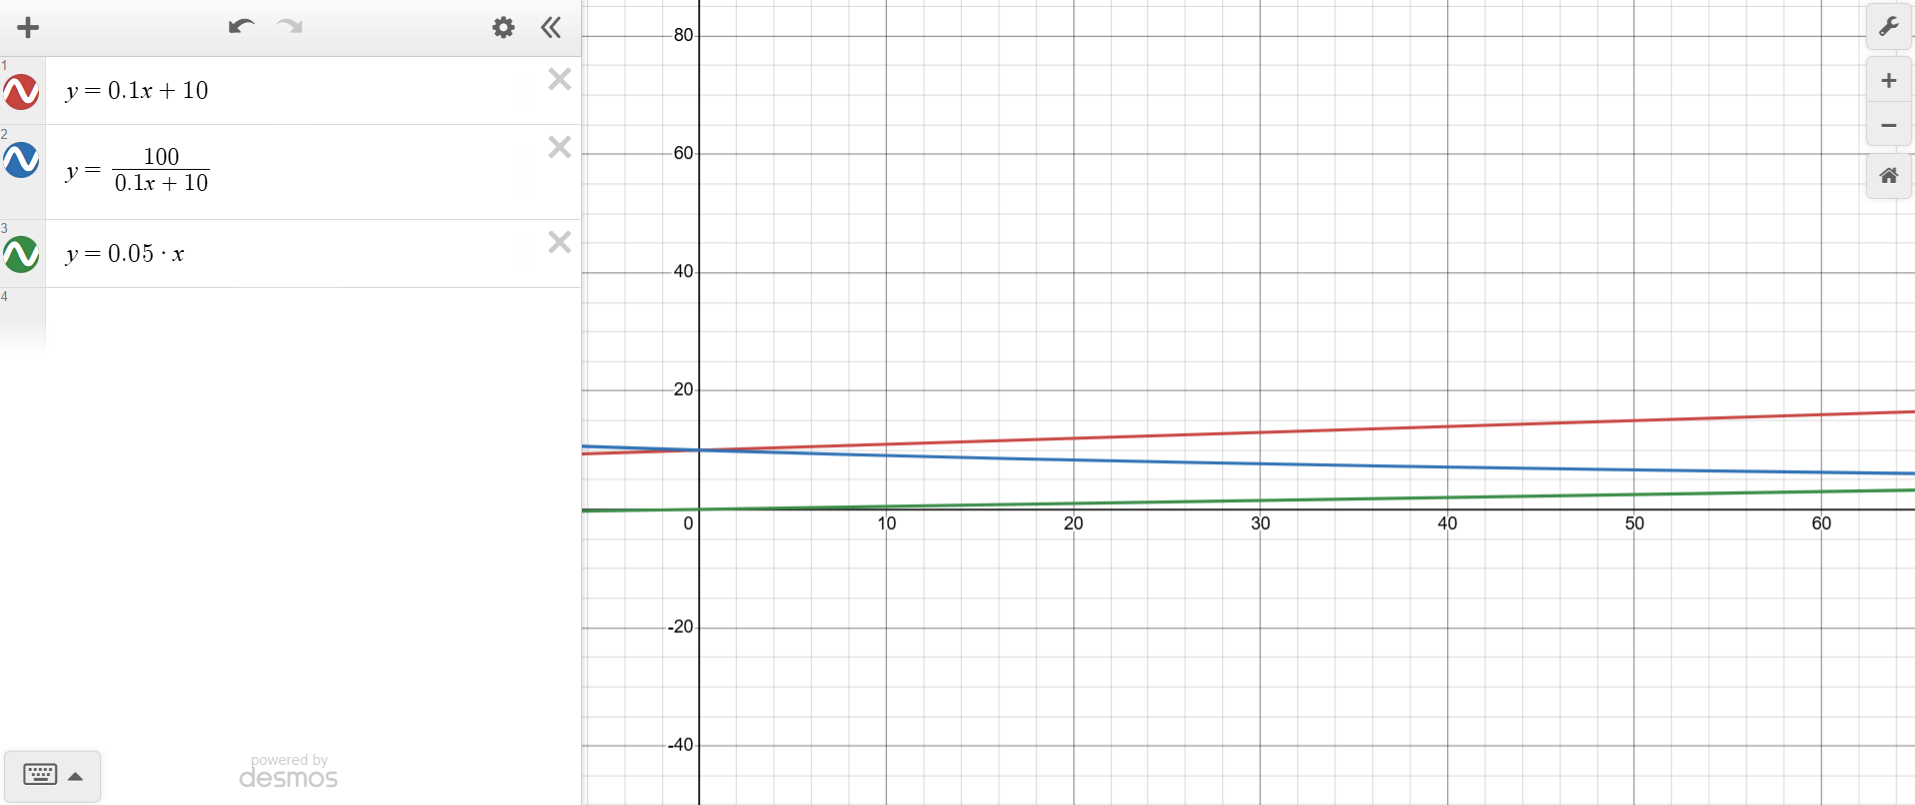
\includegraphics[width=1\textwidth]{images/graf_elo_calc.png}
    \caption{Wykres przedstawia zmiane punktacji ELO w zależności od różnicy poziomu graczy. \\ Wykresy utworzone za pomocą strony www.desmos.com}
\end{figure}
\vspace{1cm}

\noindent
System ELO w aplikacji jest zoptymalizowany, aby sprawiedliwie odzwierciedlać wyniki rozgrywek. Wzory uwzględniają różnicę umiejętności między graczami, nagradzając trudniejsze zwycięstwa i minimalizując znaczenie wyników oczekiwanych. Dzięki tym zasadom system punktacji motywuje graczy do rozwoju i rywalizacji, zachowując jednocześnie równowagę w ocenie ich umiejętności.
\\\\

\noindent \textbf{Punktacja gry z silnikiem}\\
Punktacja ELO w przypadku gier z silnikiem różni się od tej stosowanej w grach między graczami. Ma ona charakter symboliczny i informacyjny, a jej celem jest głównie odzwierciedlenie wyniku starcia z komputerowym przeciwnikiem. Wyniki z gier z silnikiem nie są uwzględniane w oficjalnych rankingach aplikacji. Mechanizm ten działa w następujący sposób: w zależności od poziomu silnika (od 1 do 20), punktacja jest modyfikowana odpowiednio do wyniku gry. Jeśli gracz przegra z silnikiem, od jego ELO jest odejmowany poziom silnika, natomiast jeśli gracz wygra, do jego ELO jest dodawany poziom silnika. Dzięki temu użytkownicy mogą w przybliżeniu ocenić swoje umiejętności względem różnych poziomów trudności silnika, co może stanowić dla nich dodatkową motywację i wskaźnik postępu.

\newpage

\noindent \textbf{Zarządzanie czasem gry}\\
W szachach istnieje kilka różnych typów ustawienia czasu, które mają wpływ na dynamikę gry. W zależności od wybranego typu, gracze mają różne limity czasowe na wykonanie swoich ruchów. Każdy z tych typów jest dostosowany do innego tempa rozgrywki, co pozwala na dopasowanie doświadczenia gry do preferencji graczy. Czas gry w szachach może obejmować różne długości, poczynając od błyskawicznych partii typu "Bullet", po długoterminowe gry "Daily", gdzie gracze wykonują ruchy w ciągu wielu dni.
\\\\
Poniżej przedstawiona jest tabela pokazująca różne kategorie kontroli czasowych:

\renewcommand{\arraystretch}{1.5}
\begin{table}[h!]
    \centering
    \begin{tabular}{|l|m{3cm}|m{3cm}|m{5cm}|}
        \hline
        \rowcolor{lightgray}
        \textbf{Typ Czasu} & \textbf{Zakres Czasu} & \textbf{Inkrement} & \textbf{Charakterystyka} \\ \hline
        \textbf{Bullet} & 1 - 3 min. & 0 - 60 sek. & Bardzo szybka gra. \\ \hline
        \textbf{Blitz} & 3 - 10 min. & 0 - 60 sek. & Gra o szybkim tempie. \\ \hline
        \textbf{Rapid} & 10 - 60 min. & 0 - 60 sek. & Gra o średnim tempie. \\ \hline
        \textbf{Classic} & 60 - 1440 min. & 0 - 60 sek. & Dużą ilością czasu. \\ \hline
        \textbf{Daily} & $\geq$ 1440 min. & 0 - 60 sek. & Bardzo długi czas gry. \\ \hline
    \end{tabular}
    \caption{Rodzaje kontroli czasowej gry.}
\end{table}
\vspace{0.5cm}

\noindent
Podczas pierwszego pobrania gry przez graczy ustalany jest czas rozpoczęcia partii. Następnie, przy każdym wykonanym ruchu, system oblicza, ile czasu minęło od ostatniego zarejestrowanego momentu (czy to od rozpoczęcia gry, czy od ostatniego ruchu). Na podstawie tej różnicy czasu, system aktualizuje pozostały czas dla gracza, odejmując upływający czas od jego pozostałego limitu. Dodatkowo, po każdym ruchu do czasu pozostałego dla gracza dodawany jest inkrement. Czas jest aktualizowany osobno dla każdego z graczy, w zależności od tego, która tura jest aktualnie wykonywana.

\vspace{0.5cm}
\begin{figure}[h!]
    \centering
    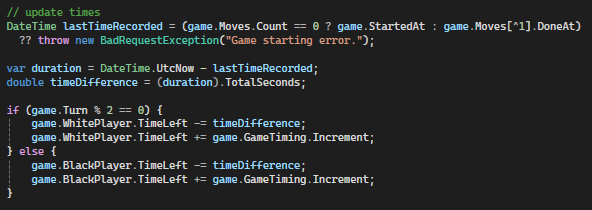
\includegraphics[width=0.7\textwidth]{images/ex_update_times.png}
    \caption{Fragment kodu: Aktualizacje czasu graczy.}
\end{figure}
\vspace{0.5cm}

Aplikacja posiada także zaimplementowane zadanie cykliczne, które jest uruchamiane co minutę, aby monitorować postęp czasu w długoterminowych trybach gry, takich jak "Classic" i "Daily", ale także do pozostałych trybów. Zadanie to sprawdza, czy któremuś z graczy nie skończył się czas, co powinno skutkować zakończeniem gry. System analizuje, kiedy ostatni ruch został zarejestrowany i oblicza różnicę między tym czasem a bieżącym czasem. Na tej podstawie, dla każdego gracza obliczany jest pozostały czas, a jeżeli czas gracza którego jest tura upłynie, system kończy grę.

\newpage

\subsubsection{Pozostałe kluczowe aspekty}

\noindent \textbf{Przetwarzanie zapytań}\\
W systemie przetwarzania zapytań wykorzystywana jest biblioteka \textbf{MediatR}, która umożliwia zarządzanie zapytaniami w sposób przejrzysty i modularny. MediatR opiera się na wzorcu projektowym Mediatora, co pozwala na oddzielenie logiki przetwarzania zapytań od innych komponentów aplikacji.
\\\\
W tym systemie każde zapytanie, pobrania danych lub zapisania ich, jest reprezentowane przez obiekt, który dziedziczy po interfejsie \texttt{IRequest<T>}, gdzie \texttt{T} oznacza typ odpowiedzi, którą zapytanie zwróci. Zapytania te są przekazywane do mediatorów, którzy następnie kierują je do odpowiednich handlerów, czyli klas odpowiedzialnych za wykonanie logiki związanej z zapytaniem.
\\\\

\textbf{Przebieg przetwarzania zapytania}
\begin{enumerate}
    \item \textbf{Zgłoszenie zapytania:} Kiedy klient wyśle zapytanie do systemu przez API lub SignalR, zapytanie to jest mapowane na odpowiedni Request, który może zawierać dane wejściowe potrzebne do przetworzenia.
    \item \textbf{Przetwarzanie zapytania:} Zapytanie trafia do MediatR, który przekazuje je do odpowiedniego handlera. Handler jest odpowiedzialny za wykonanie logiki biznesowej.
    \item \textbf{Wykonanie akcji:} Handler wykonuje określoną akcję. Może to być np. zapis do bazy danych, obliczenie wyniku gry, aktualizacja punktacji ELO lub inne działania biznesowe.
    \item \textbf{Zwrócenie odpowiedzi:} Po wykonaniu akcji, handler zwraca odpowiedź (np. dane w formie obiektu, kod statusu, wynik operacji). MediatR przekazuje tę odpowiedź z powrotem do klienta.
\end{enumerate}

\noindent
W systemie, który obsługuje zapytania, każde zapytanie jest reprezentowane przez osobny obiekt zapytania, który jest mapowany na Request. Każdy Request posiada przypisany handler, który odpowiedzialny jest za realizację zapytania.
\\\\

\textbf{Zalety wykorzystania MediatR:}
\begin{itemize}
    \item \textbf{Separation of Concerns:} MediatR pozwala na oddzielenie logiki przetwarzania zapytań od innych części aplikacji, takich jak kontrolery czy warstwa interfejsu użytkownika.
    \item \textbf{Skalowalność i modularność:} Dzięki wykorzystaniu handlerów, system jest łatwiejszy do rozszerzania i utrzymania. Każda operacja jest odseparowana w osobnym komponencie, co ułatwia zarządzanie kodem.
    \item \textbf{Testowalność:} Każdy handler można testować niezależnie, co ułatwia implementację testów jednostkowych.
    \item \textbf{Centralizacja logiki:} Logika biznesowa jest centralizowana w handlerach, co zapewnia spójność i łatwość w zarządzaniu.
\end{itemize}

\newpage

\noindent
Proces przetwarzania zapytania w systemie został szczegółowo przedstawiony na poniższym diagramie. Ukazuje on pełny przepływ danych, rozpoczynając od wysłania żądania HTTP przez klienta. Następnie żądanie jest odbierane przez odpowiedni punkt końcowy API lub metodę Huba SignalR, który przetwarza przesłany model danych. Model ten jest mapowany na obiekt zapytania (Request), który definiuje szczegóły operacji do wykonania.
\\\\
Zapytanie trafia do handlera, który obsługuje żądanie i wykonuje określoną logikę biznesową. W przypadku konieczności dostępu do danych, handler korzysta z repozytorium, które odpowiada za interakcję z bazą danych. Dane pobrane w formie encji są następnie mapowane na obiekt DTO (Data Transfer Object), który stanowi zwracany wynik. 
\\\\
Finalnie odpowiedź w postaci DTO jest zwracana przez punkt końcowy API do klienta, który otrzymuje wynik operacji w formacie zgodnym z jego wymaganiami. Diagram ten ilustruje całość procesu, uwzględniając jego modularność i spójność.

\vspace{1cm}
\begin{figure}[h!]
    \centering
    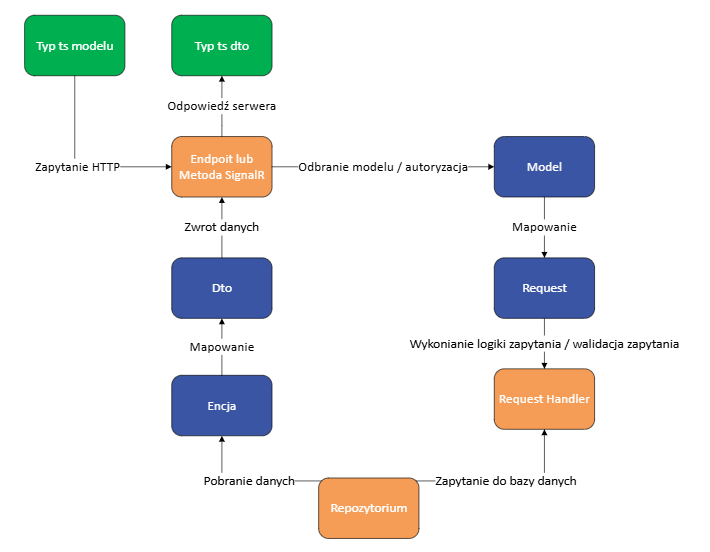
\includegraphics[width=1\textwidth]{images/diagram_back.png}
    \caption{Diagram przedstawiający proces przetwarzania zapytania na serwerze. Opracowany za pomocą aplikacji Viso.}
\end{figure}

\newpage

\noindent \textbf{Rezultaty zapytań i paginacja}\\
W systemie, zwracane są także odpowiedzi, które mogą zawierać dane w różnych formach. W przypadku wielu zapytań, szczególnie tych związanych z wyszukiwaniem lub pobieraniem dużej ilości danych, wykorzystuje się specjalne klasy, które umożliwiają mapowanie wyników na odpowiednie modele. Część zapytań zwraca dane w postaci \textbf{DTO (Data Transfer Object)}, które są prostymi obiektami przechowującymi dane. Te obiekty są mapowane z encji bazy danych, co pozwala na łatwiejsze i bardziej kontrolowane przekazywanie danych pomiędzy warstwami aplikacji.
\\\\
W przypadku, gdy zapytanie dotyczy wielu elementów (np. listy gier), zastosowana jest paginacja – technika, która pozwala na dzielenie dużych zbiorów danych na mniejsze części, co znacznie poprawia wydajność i doświadczenie użytkownika, ograniczając ilość danych przesyłanych w jednym żądaniu. Dzięki paginacji zamiast zwracać wszystkie dane na raz, system zwraca tylko określoną liczbę elementów na stronie oraz informację o numerze strony. Dzięki temu, gdy liczba elementów jest duża, użytkownik może nawigować po wynikach w sposób bardziej wydajny, ładować tylko potrzebne dane i nie obciążać systemu nadmiernym przesyłaniem informacji.
\\\\
Aby wspierać paginację, w systemie zostały zaimplementowane dwie klasy:
\begin{itemize}
    \item \textbf{PagedRequest:} Ogólna klasa, z której dziedziczą modele i zapytania wymagające paginacji. Zawiera parametry określające numer strony oraz rozmiar strony, które są używane do obliczenia, które elementy mają zostać zwrócone.
    \item \textbf{PagedResult<T>:} Klasa, która jest używana do zwracania wyników zapytania z paginacją. Przyjmuje generyczny typ T, który odpowiada za dane zwracane w odpowiedzi, takie jak DTO. Klasa ta zawiera szczegóły dotyczące wyników: listę elementów, łączną liczbę stron, numerację wyników oraz całkowitą liczbę elementów.
\end{itemize}

\begin{figure}[h!]
    \centering
    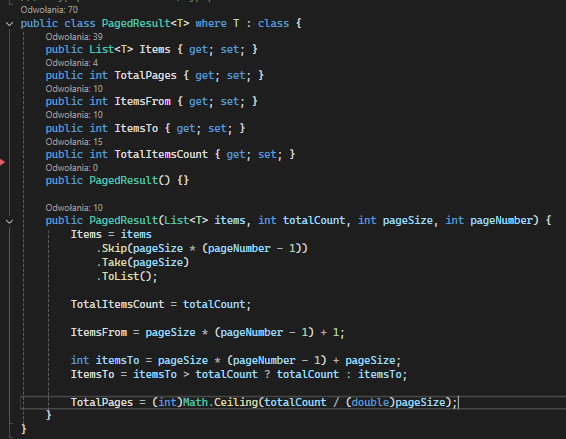
\includegraphics[width=0.7\textwidth]{images/ex_pagination.png}
    \caption{Klasa rezultatu paginacji.}
\end{figure}

\newpage

\noindent
Poniższe ilustracje przedstawiają strukturę modelu używanego w systemie. Po lewej stronie znajduje się definicja modelu w TypeScript, wykorzystywana po stronie klienta, natomiast po prawej widoczny jest odpowiednik tego modelu w kodzie zaplecza, który reprezentuje dane w aplikacji po stronie serwera.

\vspace{1cm}
\begin{minipage}[t]{0.45\textwidth} 
    \vspace{0pt} 
    \centering 
    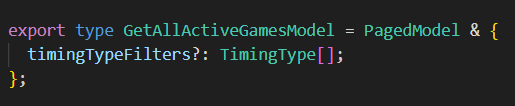
\includegraphics[width=\linewidth]{images/ex_model_front.png} 
    Fragment kodu: Przykład modelu danych klienta (TypeScript)
\end{minipage} 
\hfill 
\begin{minipage}[t]{0.45\textwidth} 
    \vspace{0pt} 
    \centering 
    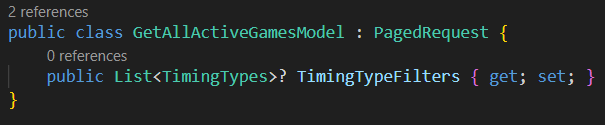
\includegraphics[width=\linewidth]{images/ex_model_back.png} 
    Fragment kodu: Przykład modelu danych serwera (C\#)
\end{minipage} 
\vspace{1cm}

\noindent
Rysunek poniżej przedstawia strukturę obiektu żądania. Obiekt ten przenosi dane wejściowe od punktu końcowego API do handlera, który wykonuje logikę biznesową.

\vspace{1cm}
\begin{figure}[h!]
    \centering
    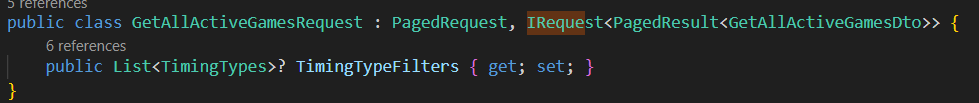
\includegraphics[width=1\textwidth]{images/ex_request_back.png}
    \caption{Fragment kodu: Struktura obiektu żądania (Request)}
\end{figure}
\vspace{1cm}

\noindent
Kolejne diagramy ilustrują przykładowe obiekty DTO. Po lewej stronie widoczny jest obiekt używany w warstwie zaplecza, który mapuje dane encji pobrane z bazy. Po prawej znajduje się odpowiedni typ w TypeScript, który reprezentuje te dane po stronie klienta.

\vspace{1cm}
\begin{minipage}[t]{0.45\textwidth} 
    \vspace{0pt} 
    \centering 
    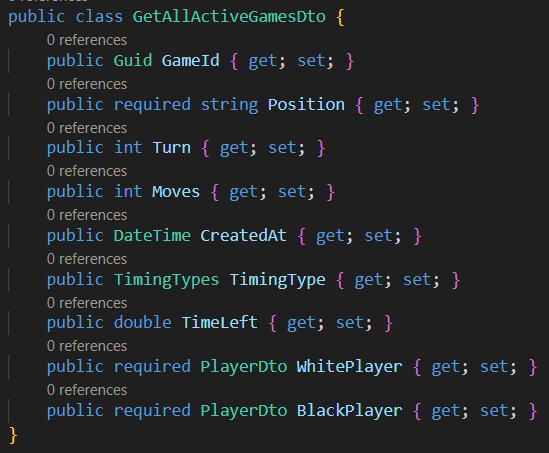
\includegraphics[width=\linewidth]{images/ex_dto_back.png} 
    Fragment kodu: DTO w warstwie serwerowej (C\#)
\end{minipage} 
\hfill 
\begin{minipage}[t]{0.45\textwidth} 
    \vspace{0pt} 
    \centering 
    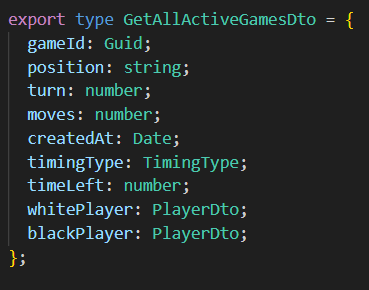
\includegraphics[width=\linewidth]{images/ex_dto_front.png} 
    Fragment kodu: DTO w warstwie klienta (TypeScript)
\end{minipage}

\newpage

\noindent \textbf{Serwis SMTP}\\
Serwis SMTP (Simple Mail Transfer Protocol) jest wykorzystywany w aplikacji do obsługi wysyłania wiadomości e-mail, co obejmuje zarówno proces weryfikacji e-maila użytkowników, jak i powiadamianie o zaproszeniach do gry. W aplikacji implementacja serwisu SMTP umożliwia automatyczne generowanie i wysyłanie e-maili w różnych scenariuszach, takich jak potwierdzenie rejestracji, resetowanie hasła, czy zaproszenia do gier.
\\\\
Serwis SMTP, za pomocą klasy SmtpService, korzysta z biblioteki .NET, która umożliwia konfigurację połączeń z serwerem pocztowym i wysyłanie e-maili. Serwis ten jest skonfigurowany przy użyciu opcji zawartych w appsettings.json, który przechowuje dane potrzebne do połączenia z serwerem SMTP (adres hosta, port, dane logowania, itp.).
\\\\
Serwis implementuje kilka kluczowych metod umożliwiających wysyłkę maili, służących do weryfikacji lub otrzymywania powiadomień. Wszystkie metody w serwisie tworzą wiadomość e-mail, której treść jest zbudowana w formacie HTML, co umożliwia bardziej zaawansowane formatowanie, w tym wstawianie obrazków, linków czy kodów.
\\\\
Wszystkie e-maile są wysyłane przez SmtpClient, który łączy się z odpowiednim serwerem SMTP (na podstawie danych konfiguracyjnych) i wysyła wiadomość do wskazanego odbiorcy. Dzięki asynchroniczności operacji, wysyłanie e-maili nie blokuje głównego wątku aplikacji, co zapewnia płynność działania systemu.
\\\\

\noindent \textbf{Serwis JWT}\\
Serwis JWT (JSON Web Token) w aplikacji służy do generowania tokenów autoryzacyjnych, które są wykorzystywane do uwierzytelniania użytkowników oraz zapewnienia dostępu do chronionych zasobów aplikacji. Tokeny JWT są powszechnie stosowane w aplikacjach webowych do obsługi logowania i autoryzacji, a ich głównym celem jest umożliwienie użytkownikowi dostępu do określonych zasobów, bez konieczności ponownego wprowadzania danych logowania przy każdym żądaniu.
\\\\
Implementacja serwisu JWT w aplikacji opiera się na klasie, która zawiera metodę GetJwtToken. Metoda ta przyjmuje obiekt User, który reprezentuje zalogowanego użytkownika, a na podstawie jego danych generuje unikalny token. Serwis ten generuje tokeny uwierzytelniające użytkowników. Na początku tworzy zestaw roszczeń, takich jak identyfikator, nazwa użytkownika, rola i status weryfikacji e-maila. Token jest podpisywany za pomocą klucza przechowywanego w ustawieniach aplikacji, używając algorytmu HMAC-SHA256. Określana jest również data wygaśnięcia tokenu, np. po 7 dniach. Następnie tworzony jest obiekt JwtSecurityToken, który zawiera claims, datę wygaśnięcia i podpisane dane. Token jest serializowany do formatu string i przesyłany w odpowiedzi do klienta.
\\\\
Serwis JWT stanowi kluczowy element systemu autoryzacji w aplikacji, umożliwiając bezpieczne zarządzanie dostępem do chronionych zasobów w systemie. Użytkownicy, którzy zalogują się do aplikacji, otrzymują token JWT, który musi być dołączony do każdego żądania do API, aby potwierdzić tożsamość i autoryzację.

\newpage

\noindent \textbf{Entity Framework}\\
Entity Framework (EF) to nowoczesny framework ORM (Object-Relational Mapping) opracowany przez Microsoft, który umożliwia programistom łatwe mapowanie struktur danych obiektowych na tabele relacyjnej bazy danych. W aplikacji wykorzystuje się EF do zarządzania danymi oraz interakcji z bazą danych PostgreSQL w sposób obiektowy. Dzięki EF operacje na danych stają się prostsze i bardziej czytelne, eliminując potrzebę pisania ręcznych zapytań SQL.
\\\\
Podstawą działania EF jest klasa kontekstu, która w aplikacji została zaimplementowana jako \textbf{ChessAppDbContext : DbContext}. Kontekst bazy danych zarządza połączeniem z bazą danych oraz umożliwia wykonywanie operacji CRUD na encjach. W aplikacji konfiguracja każdej encji odbywa się za pomocą dedykowanej klasy \textbf{DbContextConfiguration } implementującej interfejs \textbf{IEntityTypeConfiguration<T>}. W tej konfiguracji definiowane są szczegóły dotyczące mapowania encji na tabele, takie jak nazwy kolumn, klucze główne czy relacje między tabelami.
\\\\
Dla każdej encji w aplikacji zostało utworzone dedykowane repozytorium, które jest odpowiedzialne za wykonywanie operacji na danych. Każde repozytorium posiada odpowiadający mu interfejs znajdujący się w warstwie .Application. Repozytoria pełnią rolę abstrakcyjnej warstwy dostępu do danych, umożliwiając wykonywanie operacji takich jak dodawanie, usuwanie, modyfikowanie i pobieranie danych z bazy. Repozytoria zwiększają przejrzystość kodu, separując logikę dostępu do danych od reszty aplikacji, a także ułatwiają testowanie dzięki możliwości wprowadzania mocków.
\\\\
Wszystkie elementy związane z EF i repozytoriami są rejestrowane w kontenerze IoC (Inversion of Control) za pomocą metody rozszerzającej AddPostgres. Poniżej znajduje się przykład implementacji rejestracji:

\vspace{0.5cm}
\begin{figure}[h!]
    \centering
    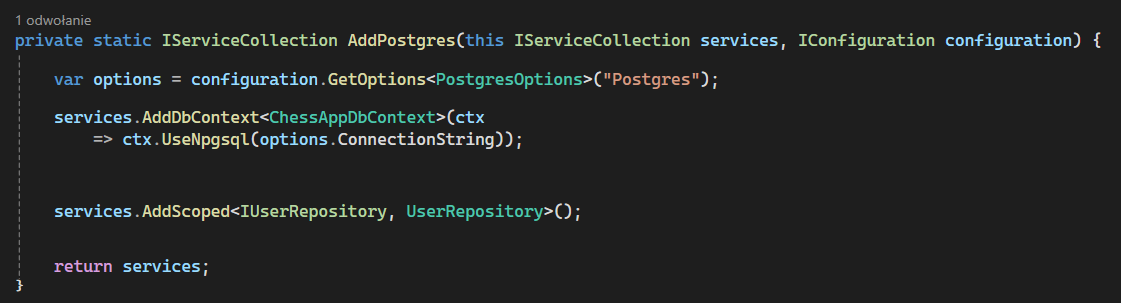
\includegraphics[width=1\textwidth]{images/ex_infra_extensions.png}
    \caption{Fragment kodu: Rejestracja kontekstu oraz repozytoriów.}
\end{figure}
\vspace{0.5cm}

Metoda ta umożliwia skonfigurowanie połączenia z bazą PostgreSQL oraz rejestrację wszystkich repozytoriów w kontenerze usług, dzięki czemu są one dostępne w całej aplikacji. Takie podejście wspiera modularność oraz ułatwia zarządzanie zależnościami.

\newpage

\noindent \textbf{Zadania cykliczne}\\
Zadania cykliczne w projekcie to procesy działające w tle, które są wykonywane w określonych odstępach czasu bez konieczności interakcji użytkownika. W aplikacji takie zadania realizuje się za pomocą klasy, która dziedziczy po \textbf{BackgroundService}. Dzięki temu mechanizmowi zadania te są uruchamiane automatycznie podczas działania aplikacji i wykonują swoją logikę w nieskończonej pętli, z uwzględnieniem przerw między iteracjami.
\\\\
W projekcie zadanie cykliczne odpowiedzialne jest za monitorowanie i automatyczne kończenie gier sieciowych, które spełniają określone warunki. Do jego realizacji wykorzystano wstrzykiwanie zależności, umożliwiając dostęp do dedykowanego serwisu wykonującego kluczowe operacje. Takie podejście pozwala na regularne przetwarzanie danych w tle, co wpływa na płynność działania aplikacji i automatyzację procesów.
\\\\
W metodzie \textbf{ExecuteAsync} wykonywana jest nieskończona pętla, która co 60 sekund wywołuje metodę \textbf{FinishGames}. Metoda ta korzysta z serwisu \textbf{IWebGamesFinisherService} za pomocą mechanizmu dependency injection, aby zrealizować logikę kończenia gier. Sam serwis został zaimplementowany w celu automatycznego kończenia gier o długiej kontroli czasowej, aby zapobiegać pozostawianiu nierozstrzygniętych rozgrywek i utrzymywać porządek w systemie, ale także aby rozstrzygać gry krótkoterminowe, których zawodnik opuścił partię w nieprawidłowy sposób.
\\\\

\noindent \textbf{Obsługa błędów}\\
Obsługa błędów w projekcie została zaprojektowana w sposób centralny, co ułatwia zarządzanie wyjątkami i poprawia doświadczenie użytkownika. Wykorzystuje się w tym celu middleware, który przechwytuje wszystkie wyjątki generowane podczas obsługi żądań i mapuje je na odpowiednie kody statusu HTTP.
\\\\
Dzięki temu podejściu różne typy wyjątków (np. błędy użytkownika, brak zasobu, brak autoryzacji) są konwertowane na czytelne i spójne odpowiedzi dla klienta. Centralizacja obsługi błędów zwiększa przejrzystość kodu i umożliwia szybsze rozwiązywanie problemów, ponieważ wszystkie wyjątki są przetwarzane w jednym miejscu.
\\\\
Obsługa błędów w projekcie została zaimplementowana za pomocą klasy \textbf{ExceptionMiddleware}, która pełni rolę middleware w aplikacji ASP.NET Core. Middleware przechwytuje wszystkie wyjątki, które mogą wystąpić podczas obsługi żądań HTTP, i mapuje je na odpowiednie kody statusu HTTP:

\begin{itemize}
    \item \textbf{400 (Bad Request):} dla wyjątków BadRequestException, gdy żądanie jest niepoprawne.
    \item \textbf{404 (Not Found):} dla wyjątków NotFoundException, gdy żądany zasób nie istnieje.
    \item \textbf{401 (Unauthorized):} dla wyjątków UnauthorizedException, gdy użytkownik nie jest autoryzowany.
    \item \textbf{500 (Internal Server Error):} dla wszystkich pozostałych nieobsłużonych błędów.
\end{itemize}

\newpage

\subsubsection{Wykorzystane pakiety i biblioteki}

W projekcie zastosowano szereg bibliotek, które wspierają rozwój i funkcjonalność aplikacji. Każda z wymienionych bibliotek została dobrana w celu spełnienia konkretnych wymagań funkcjonalnych i architektonicznych projektu, co pozwala na jego rozwój zgodny z najlepszymi praktykami. Poniżej przedstawiono szczegółowy opis wybranych komponentów:
\begin{itemize} 
    \item \textbf{Swashbuckle.AspNetCore} i \textbf{SignalRSwaggerGen}: Obie biblioteki służą do generowania dokumentacji Swagger, co pozwala na dokumentowanie API REST i SignalR w jednej konfiguracji. 
    \item \textbf{AutoMapper}: Biblioteka umożliwiająca mapowanie obiektów między różnymi warstwami aplikacji, eliminując potrzebę ręcznego mapowania. 
    \item \textbf{MediatR}: Implementuje wzorzec Mediatora, co umożliwia luźne powiązanie komponentów aplikacji i jest powszechnie wykorzystywane w aplikacjach opartych na wzorcu CQRS. 
    \item \textbf{Npgsql.EntityFrameworkCore.PostgreSQL} i \textbf{Microsoft.EntityFrameworkCore}: Npgsql to dostawca dla Entity Framework Core dla bazy danych PostgreSQL, co umożliwia korzystanie z tej bazy danych za pomocą EF Core w aplikacjach .NET. 
    \item \textbf{FluentAssertions}: Biblioteka do tworzenia bardziej czytelnych i wyrażających zamiar asercji w testach jednostkowych. 
    \item \textbf{Microsoft.AspNetCore.SignalR} i \textbf{Microsoft.AspNetCore.Cors}: Obie biblioteki obsługują komunikację w czasie rzeczywistym oraz kontrolują dostęp do zasobów serwera z innych domen w aplikacjach webowych. 
    \item \textbf{Microsoft.AspNetCore.Identity} i \textbf{Microsoft.AspNetCore.Authentication.JwtBearer}: Biblioteki związane z bezpieczeństwem aplikacji, wspierające mechanizmy uwierzytelniania i autoryzacji, w tym logowanie z użyciem JWT. 
    \item \textbf{Microsoft.AspNetCore.Mvc.Core} i \textbf{Microsoft.AspNetCore.Mvc.Testing}: Obie biblioteki są odpowiedzialne za budowanie endpointów API oraz testowanie aplikacji, w tym kontrolerów i routingu. 
    \item \textbf{Microsoft.IdentityModel.Tokens}: Biblioteka do obsługi tokenów, takich jak JWT, niezbędna do tworzenia i weryfikacji tokenów w aplikacjach z uwierzytelnianiem opartym na tokenach. 
    \item \textbf{Microsoft.Extensions.*}: Zestaw bibliotek wspierających konfigurację aplikacji oraz wstrzykiwanie zależności, kluczowy dla budowy skalowalnych aplikacji.
    \item \textbf{Microsoft.NET.Test.Sdk}, \textbf{xUnit}, \textbf{xUnit.runner.visualstudio} i \textbf{Moq}: Zestaw bibliotek do testowania aplikacji, wspierający tworzenie testów jednostkowych i integracyjnych, w tym generowanie mocków i uruchamianie testów w Visual Studio. 
\end{itemize}

\newpage
\subsection{Warstwa Kliencka (Frontend)}
\subsubsection{Architektura i struktura}

Struktura frontendu w tym projekcie jest zorganizowana w sposób umożliwiający łatwe zarządzanie kodem, dzięki zastosowaniu odpowiednich folderów i podfolderów, które odpowiadają za różne aspekty aplikacji. W głównym folderze \textbf{src} znajdują się trzy główne foldery oraz pliki aplikacji. Każdy z folderów ma swoją specyficzną rolę w organizacji kodu.
\\\\
Folder \textbf{index} zawiera router odpowiedzialny za strony ogólnodostępne, takie jak strona główna, rejestracja czy informacje o aplikacji. Folder \textbf{main} jest przeznaczony do zarządzania zasobami dostępnymi tylko dla zalogowanych i zweryfikowanych użytkowników. Dostęp do tych stron jest kontrolowany na podstawie stanu autoryzacji użytkownika, co zapewnia bezpieczeństwo aplikacji. Folder \textbf{shared} natomiast zawiera komponenty i funkcjonalności, które są współdzielone pomiędzy różnymi częściami aplikacji. Każda z sekcji ma wyraźnie określoną rolę i zakres odpowiedzialności, co sprzyja porządkowi w projekcie i ułatwia dalsze rozwijanie aplikacji.

\vspace{0.5cm}
\begin{figure}[h!]
    \centering
    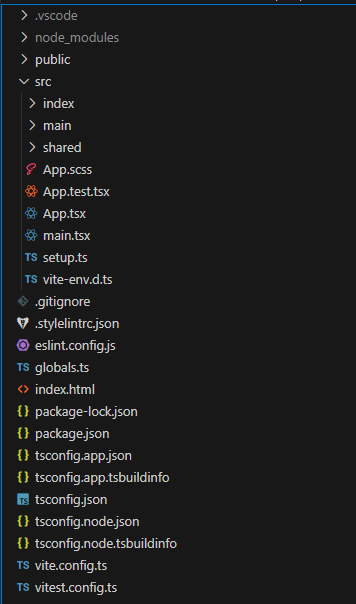
\includegraphics[width=0.5\textwidth]{images/struktura_front.png}
    \caption{Struktura projektu warstwy klienckiej.}
\end{figure}

\newpage

\noindent
Ponadto na najniższym poziomie struktury projektu dodano lub automatycznie wygenerowano szereg plików odpowiedzialnych za konfigurację zarówno samego projektu, jak i środowiska deweloperskiego.
\\\\
Folder \textbf{shared} w projekcie jest zaprojektowany w sposób, który sprzyja ponownemu wykorzystaniu kodu i organizacji wspólnych zasobów używanych w całej aplikacji. Zawiera on różnorodne podfoldery, które grupują funkcje, komponenty i style, w zależności od ich roli w projekcie.

\begin{itemize}
    \item \textbf{components:} przechowuje małe, wielokrotnie używane komponenty, które są wykorzystywane w różnych miejscach aplikacji. Mogą to być takie elementy jak  przyciski, okna ładowania czy inne fragmenty UI, które są stosowane w różnych częściach aplikacji.
    \item \textbf{styles:} zawiera globalne definicje stylów SCSS. Są tam zdefiniowane zmienne, które ułatwiają zarządzanie kolorami, czcionkami, a także mixiny, które pomagają w definiowaniu jednolitych stylów elementów. Dzięki temu stylowanie jest bardziej spójne i łatwiejsze do modyfikacji w jednym miejscu. Wszystkie współdzielone style są zbierane z różnych plików do jednego - shared.scss, ktory to następnie jest importowany do wszystkich komponentów strony aby umożliwić ich działanie.
    \item \textbf{svgs:} gromadzi wszystkie ikony i mapy ikon, które są wielokrotnie używane w aplikacji. Mapy ikon to funkcje, które na podstawie podanej nazwy ikony zwracają odpowiedni tag svg, co pozwala na łatwe zarządzanie ikonami w projekcie. Do tworzenia ikon stosowany jest specjalny komponent, ktory wymaga podania wybranej mapy oraz nazwy ikon, ktory nastepnie na podstawie tych parametrow zwraca i tworzy odpowiednia ikone.
    \item \textbf{utils:} zawiera dodatkowe narzędzia, które wspomagają działanie aplikacji. Jest podzielony na kilka podfolderów:
    \begin{itemize}
        \item \textbf{functions:} zawiera globalne i współdzielone funkcje, podzielone na pliki w zależności od ich zastosowania. Można tu znaleźć funkcje pomocnicze, które są wykorzystywane w różnych częściach aplikacji.
        \item \textbf{hooks:} zawiera niestandardowe hooki React, które są ponownie wykorzystywane w różnych komponentach. To funkcje, które upraszczają logikę i stan aplikacji.
        \item \textbf{objects:} przechowuje stałe wartości, listy, obiekty i słowniki, które są wykorzystywane w aplikacji. Może to obejmować np. stałe, które odnoszą się do kategorii, statusów czy innych danych, które są wspólne dla różnych części aplikacji.
        \item \textbf{services:} zawiera zbiory funkcji lub klasy odpowiedzialne za konkretne zadania w aplikacji. Na przykład może to być serwis do wysyłania zapytań przez SignalR, który obsługuje komunikację w czasie rzeczywistym. Może także obejmować serwisy do interakcji z backendem lub innymi zewnętrznymi usługami.
        \item \textbf{types:} zawiera wszystkie ogólne typy i interfejsy TypeScript, które są wykorzystywane w aplikacji. Obejmuje to zarówno własne definicje typów, jak i przetłumaczone modele danych i DTO z backendu. Dzięki temu struktura danych w obu aplikacji jest spójna, co minimalizuje ryzyko błędów związanych z niezgodnością typów danych.
    \end{itemize}
\end{itemize}

\noindent
Cała struktura \texttt{shared} jest zaprojektowana w sposób umożliwiający łatwe zarządzanie wspólnymi zasobami, co ułatwia utrzymanie aplikacji i jej rozwój. Zastosowanie takich podziałów pozwala na organizację kodu, który może być wielokrotnie wykorzystywany w różnych częściach projektu, co prowadzi do mniejszej duplikacji kodu oraz lepszej modularności.


\newpage
\subsubsection{Routing aplikacji}
Routing w aplikacji oparty na bibliotece react-router-dom jest kluczowym elementem zarządzania nawigacją oraz wyświetlaniem odpowiednich komponentów w zależności od adresu URL. Aplikacja jest podzielona na dwie główne sekcje routingu: ogólną i bardziej specyficzną, przeznaczoną dla głównych funkcji aplikacji. Routing w aplikacji jest podzielony na dwie główne sekcje: \texttt{Index} i \texttt{Main}. Każda z tych sekcji zarządza dostępem do różnych zasobów w zależności od stanu uwierzytelnienia użytkownika.
\\\\

\noindent
\textbf{IndexRouter} odpowiada za strony ogólnodostępne, które mogą być odwiedzane przez każdego użytkownika, bez konieczności logowania lub weryfikacji. Są to strony takie jak strona główna, rejestracja czy informacje o aplikacji. Użytkownicy mogą swobodnie przeglądać te zasoby, bez jakichkolwiek ograniczeń dostępu.

\vspace{0.5cm}
\begin{figure}[h!]
    \centering
    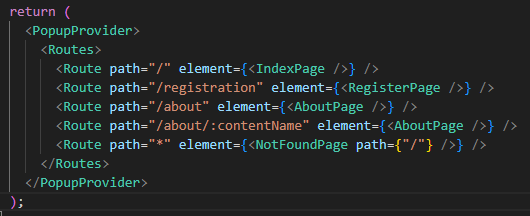
\includegraphics[width=0.7\textwidth]{images/ex_index_router.png}
    \caption{Fragment kodu: Schemat routingu dla ogólnodostępnych stron w aplikacji.}
\end{figure}

\noindent
\textbf{MainRouter} natomiast obsługuje zasoby, które są dostępne tylko dla zarejestrowanych i zweryfikowanych użytkowników. W tej części aplikacji przed uzyskaniem dostępu do stron, takich jak profil użytkownika, ranking czy gra online, aplikacja przeprowadza weryfikację, czy użytkownik jest odpowiednio zalogowany i posiada uprawnienia do korzystania z tych zasobów. Jeśli użytkownik nie spełnia wymogów autentykacji, zostaje przekierowany do odpowiednich stron, takich jak strona logowania czy rejestracji.

\vspace{0.5cm}
\begin{figure}[h!]
    \centering
    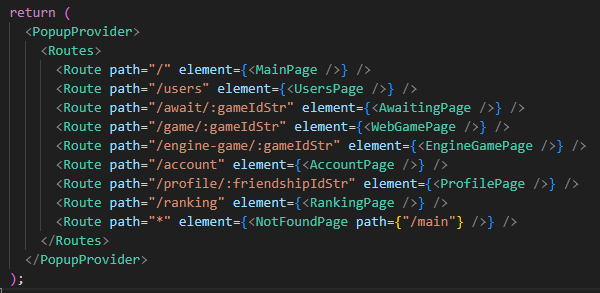
\includegraphics[width=0.7\textwidth]{images/ex_main_router.png}
    \caption{Fragment kodu: Schemat routingu dla zasobów dostępnych tylko dla zalogowanych i zweryfikowanych użytkowników.}
\end{figure}

\newpage

\noindent \textbf{Autoryzacja}\\
Autoryzacja w routerze polega na weryfikacji tokena użytkownika oraz stanu jego konta. Przy każdym wejściu na zasoby chronione, aplikacja najpierw sprawdza, czy w \texttt{localStorage} znajduje się token. Jeśli go brak, użytkownik jest przekierowywany do strony rejestracji. Następnie, jeśli token jest obecny, aplikacja sprawdza, czy adres e-mail użytkownika został zweryfikowany. W przypadku braku weryfikacji, użytkownik zostaje przekierowany do strony rejestracji z komunikatem o konieczności weryfikacji konta. Po pomyślnym zweryfikowaniu konta, aplikacja pobiera dane użytkownika, zapisuje je w lokalnym schowku i nawiązuje połączenie z serwisem gier. W przypadku jakichkolwiek problemów z autoryzacją, użytkownik jest również kierowany do strony rejestracji z odpowiednim komunikatem o błędzie.
\\\\
Poniżej przedstawiono fragment kodu z komponentu \texttt{MainRouter}, odpowiadającego za weryfikacje użytkowników.

\vspace{1cm}
\begin{figure}[h!]
    \centering
    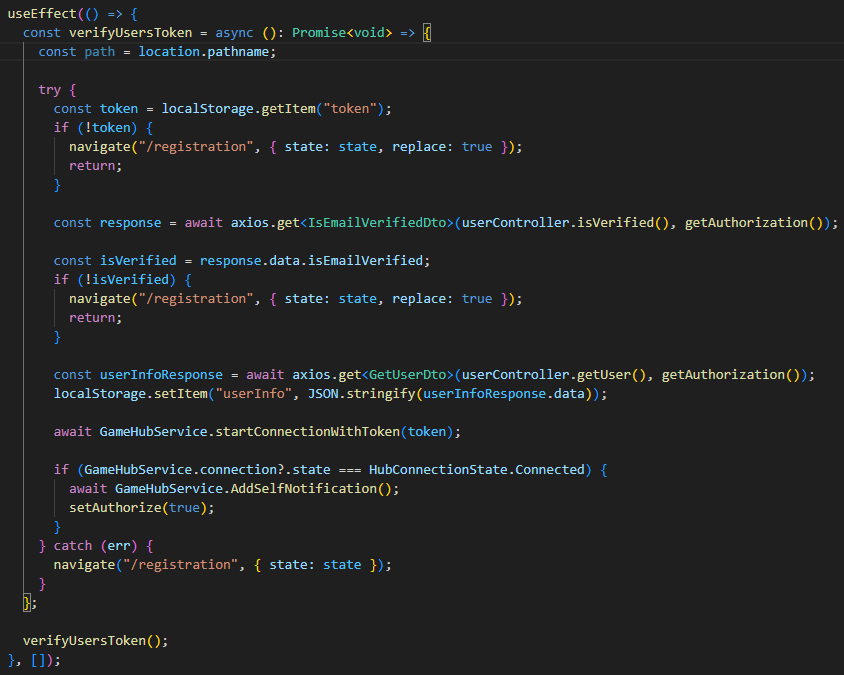
\includegraphics[width=1\textwidth]{images/ex_router_authorization.png}
    \caption{Fragment kodu: Proces autoryzacji użytkownika.}
\end{figure}

\newpage

\subsubsection{Komponenty interfejsu użytkownika}

Aplikacja korzysta z dwóch głównych routerów, z których pierwszy obsługuje strony dostępne publicznie, które stanowią wstęp do pełnej aplikacji i są dostępne bez konieczności logowania, zapewniając użytkownikom możliwość zapoznania się z funkcjami platformy przed założeniem konta. Drugi natomiast zarządza stronami, które są dostępne tylko po zalogowaniu się użytkownika i obejmują pełną funkcjonalność aplikacji. Strony te wymagają uwierzytelnienia, aby zapewnić bezpieczeństwo danych użytkowników oraz personalizację doświadczenia, co pozwala na pełne wykorzystanie możliwości aplikacji, takich jak interakcja z innymi graczami czy dostosowywanie ustawień profilu.
\\\\

\noindent \textbf{Strona tytułowa (Index)}\\
Strona tytułowa stanowi pierwsze spotkanie użytkownika z aplikacją. Zawiera ona szereg sekcji, które mają na celu zaprezentowanie aplikacji w sposób przejrzysty i zachęcający do dalszej interakcji. Sekcje na tej stronie mogą obejmować ogólne wprowadzenie do gry w szachy, zasady gry, możliwość rozpoczęcia gry online lub offline, a także funkcje aplikacji, takie jak zarządzanie znajomymi, zaproszenia do gry, czy dostęp do rankingów. Celem tej strony jest zainteresowanie użytkownika, zrozumienie, czym jest aplikacja i zachęcenie go do rejestracji lub logowania.
\\

\noindent \textbf{Strona informacyjna (About)}\\
Strona informacyjna zawiera szczegółowe informacje na temat aplikacji, jej twórców, celu, zasad działania, jak również warunki korzystania z platformy i politykę prywatności. Jest to miejsce, gdzie użytkownicy mogą zapoznać się z pełnym opisem aplikacji, jej funkcji, zasadami bezpieczeństwa oraz wymaganiami. Dzięki tej stronie użytkownik zyskuje pełen obraz tego, czego może oczekiwać od aplikacji, a także jest informowany o zasadach korzystania z usługi.
\\

\noindent \textbf{Strona do rejestracji (Register)}\\
Strona rejestracji i logowania jest kluczowym komponentem, umożliwiającym użytkownikowi utworzenie konta, zalogowanie się lub przejście przez proces weryfikacji. Ta strona składa się z jednego okna, które zmienia się dynamicznie w zależności od podjętej akcji przez użytkownika. Może to obejmować różne stany, takie jak formularz rejestracji, formularz logowania lub okno informacyjne o konieczności weryfikacji konta po jego utworzeniu. Wszystkie te akcje są obsługiwane w ramach jednego komponentu, który dynamicznie przełącza widoki w zależności od wyboru użytkownika.
\\

\noindent \textbf{Strony ładowania (Loading)}\\
Aplikacja zawiera również strony ładowania, które są wyświetlane w sytuacjach, gdy użytkownik musi poczekać na załadowanie zasobów lub wykonanie operacji, takich jak pobieranie danych z serwera. Strony te pełnią rolę informacyjną i zapewniają użytkownikowi feedback na temat aktualnego stanu procesu, na przykład ładowania gry, oczekiwania na odpowiedź z serwera lub innych operacji wymagających czasu.
\\

\noindent \textbf{Strona główna (Main)}\\
Strona główna, dostępna zaraz po zalogowaniu, stanowi centrum nawigacji aplikacji. Z jej poziomu użytkownik może rozpocząć grę, zapoznać się z historią swoich poprzednich gier, a także przejść do innych sekcji, takich jak konto użytkownika, znajomi, ranking czy ustawienia. Strona ta pełni rolę wprowadzenia do pełnej funkcjonalności aplikacji, umożliwiając użytkownikowi szybki dostęp do najistotniejszych opcji. Oprócz rozpoczęcia nowych gier i przeglądania starych, użytkownik może również zapraszać znajomych do gry lub przejrzeć dostępne tryby rozgrywki.
\\

\noindent \textbf{Strona gry online (WebGame)}\\
Jest to komponent odpowiedzialny za rozgrywki online. Mechanizm gry w tym przypadku oparty jest na interakcji dwóch graczy, którzy mogą rywalizować ze sobą w czasie rzeczywistym. Gra jest synchronizowana na bieżąco za pomocą mechanizmów, takich jak SignalR, co pozwala na natychmiastowe przesyłanie danych o wykonanych ruchach i stanie gry między użytkownikami. Strona ta oferuje interfejs umożliwiający pełną interakcję z planszą szachową, a także daje możliwość korzystania z dodatkowych funkcji, takich jak czat czy podgląd statystyk. Wygląd strony jest zoptymalizowany pod kątem dynamicznej gry online, zapewniając użytkownikowi płynne doświadczenie.
\\

\noindent \textbf{Strona gry offline (EngineGame)}\\
Ten komponent odpowiada za tryb gry z komputerem, czyli tryb offline. W tym przypadku użytkownik gra przeciwko sztucznej inteligencji (AI), a rozgrywka jest realizowana w trybie offline, bez potrzeby połączenia z innym graczem. Mechanizmy gry różnią się od tych w trybie online, gdyż cała interakcja odbywa się tylko po stronie użytkownika i aplikacji, bez wymiany danych z zewnętrznymi źródłami. Strona EngineGame jest pod względem wyglądu podobna do strony WebGame, jednak w tym przypadku użytkownik nie ma możliwości zaproszenia znajomych do gry, a interakcja opiera się wyłącznie na grze z komputerem.
\\

\noindent \textbf{Strona konta użytkownika (Account)}\\
Strona konta użytkownika to miejsce, w którym użytkownik może przeglądać i edytować swój profil. Zawiera ona informacje na temat użytkownika, takie jak nazwa, e-mail, zdjęcie profilowe oraz inne szczegóły, które można zmieniać. Dodatkowo, użytkownik ma dostęp do ustawień konta, takich jak zmiana hasła czy preferencje dotyczące powiadomień. Strona ta zawiera również sekcję z podsumowaniem statystyk gracza – liczba wygranych gier, ranking, liczba rozegranych partii i inne osiągnięcia.
\\

\noindent \textbf{Strona zarządzania znajomymi (Users)}\\
Umożliwia ona użytkownikowi zarządzanie znajomymi i zapraszanie nowych osób do gry. Na tej stronie użytkownik może przeglądać swoich znajomych, wyszukiwać innych graczy, a także zapraszać ich do gry. Jest to także miejsce, gdzie można przeglądać historię zaproszeń i statusy graczy (czy są online, czy dostępni do gry). Użytkownik ma możliwość usuwania znajomych lub zatwierdzania nowych zaproszeń.
\\

\noindent \textbf{Strona profilu znajomego (Profile)}\\
Strona ta pozwala na podgląd profili innych użytkowników. Dzięki tej stronie użytkownik może zapoznać się z danymi innych graczy, ich statystykami, historią gier oraz osiągnięciami. Umożliwia to łatwiejsze nawiązanie kontaktu i zaproszenie do gry. Strona ta pełni funkcję informacyjną, pozwalając użytkownikowi lepiej poznać innych graczy i ich styl gry.
\\

\noindent \textbf{Strona rankingu (Ranking)}\\
Strona rankingu pokazuje aktualne rankingi graczy, zarówno na poziomie globalnym, jak i wśród znajomych. Użytkownik może przeglądać globalne rankingi, zobaczyć, jak plasuje się w porównaniu do innych graczy na całym świecie, jak również sprawdzić wyniki swoich znajomych. Ranking jest aktualizowany na bieżąco, odzwierciedlając wyniki wszystkich gier rozegranych w aplikacji. Dzięki temu użytkownicy mogą śledzić swoje postępy i starać się poprawić swoją pozycję w rankingu.

\newpage

\noindent \textbf{Strona błędu (NotFoundPage)}\\
Strona błędu wyświetla się, gdy użytkownik próbuje uzyskać dostęp do nieistniejącej lub niedostępnej ścieżki w aplikacji. Jest to komponent informujący użytkownika o błędnym adresie URL lub próbie dostępu do zasobu, który został usunięty lub zmieniony. Strona ta zawiera czytelny komunikat o błędzie, taki jak "404 - Strona nie znaleziona", a także odnośnik umożliwiający powrót do strony głównej lub innego zasobu aplikacji. Dzięki temu użytkownik ma możliwość szybkiego odzyskania kontroli i powrotu do korzystania z funkcjonalności aplikacji.
\\\\
Po opisaniu zasad działania routingu w aplikacji oraz przedstawieniu wszystkich głównych komponentów, warto przedstawić diagram ilustrujący strukturę nawigacji i przepływ między poszczególnymi sekcjami. Diagram ten pomoże zrozumieć zależności pomiędzy komponentami oraz sposób, w jaki routing obsługuje żądania użytkowników w zależności od ich stanu uwierzytelnienia i wymaganych uprawnień.

\vspace{1cm}
\begin{figure}[h!]
    \centering
    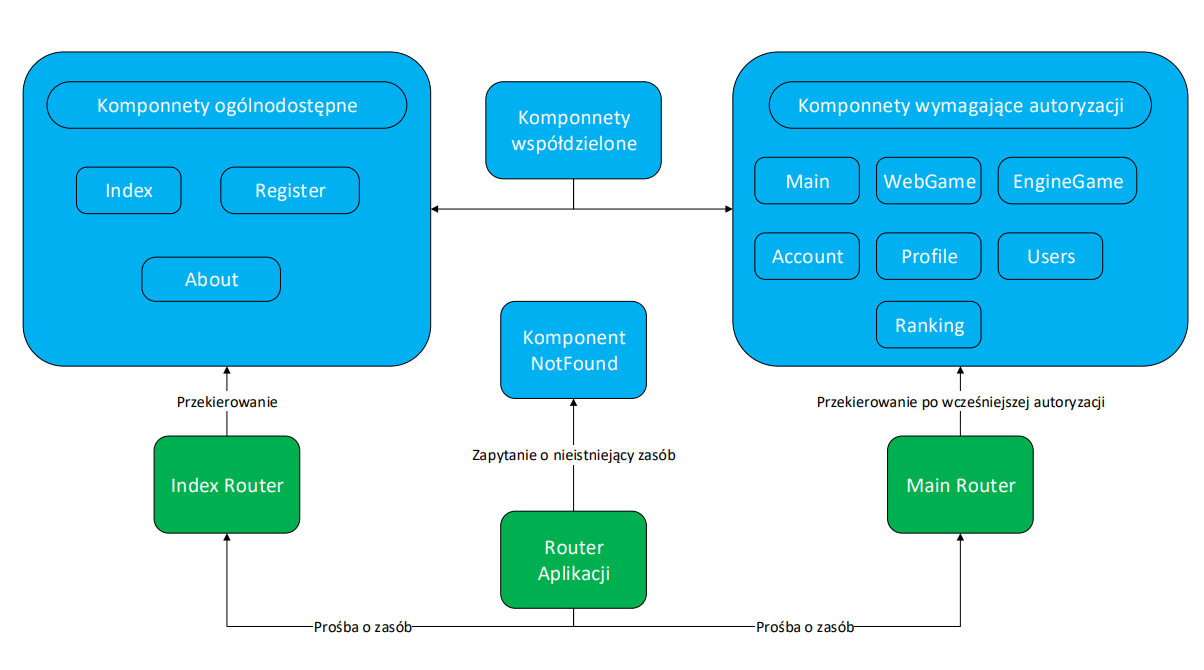
\includegraphics[width=1\textwidth]{images/diagram_routing.png}
    \caption{Diagram blokowy przedstawiający schemat routingu aplikacji. Opracowany za pomocą aplikacji Viso.}
\end{figure}

\newpage

\subsubsection{Zarządzanie stanem aplikacji}
Zarządzanie stanem aplikacji w projekcie opiera się na elastycznym wykorzystaniu kilku mechanizmów w zależności od charakteru stanu i jego zastosowania. Dzięki temu aplikacja jest w stanie skutecznie zarządzać zarówno lokalnym stanem komponentów, jak i bardziej złożonymi danymi związanymi z rozgrywką, zapewniając płynność i responsywność działania aplikacji.
\\\\
Poniżej przedstawiono szczere metod zastosowanych do zarządzania stanem aplikacji:

\begin{itemize}
    \item \textbf{Zarządzanie stanem lokalnym:} Do zarządzania stanem lokalnym, który jest związany z pojedynczymi komponentami, wykorzystywane jest \texttt{useState}. Tego typu stan przechowuje dane dotyczące interakcji użytkownika z interfejsem, na przykład wybór gry, filtrowanie wyników czy przechowywanie tymczasowych danych. Stan ten jest zmieniany w odpowiedzi na działania użytkownika lub pobieranie danych z serwera.

    \item \textbf{Zarządzanie bardziej złożonym stanem:} W przypadku bardziej skomplikowanego stanu, takiego jak stan gry, używa się \texttt{useReducer}. Ta technika pozwala na lepsze zarządzanie złożonymi i dynamicznymi danymi, takimi jak aktualny stan rozgrywki, ruchy graczy, status gry czy zmiany na planszy. Dzięki zastosowaniu reducerów możliwe jest łatwe śledzenie zmian stanu oraz utrzymywanie porządku w logice aplikacji, szczególnie w sytuacjach, gdy wiele akcji może wpływać na jeden obiekt stanu.

    \item \textbf{Globalny stan aplikacji:} Aby zarządzać danymi, które muszą być dostępne w wielu częściach aplikacji, wykorzystywany jest globalny stan oparty na \texttt{useContext} i \texttt{createContext}. Dzięki temu możliwe jest centralne przechowywanie i udostępnianie informacji, które są wykorzystywane w różnych miejscach aplikacji.

    \item \textbf{Przechowywanie danych w localStorage:} Aplikacja wykorzystuje także \texttt{localStorage} do przechowywania niektórych danych, takich jak informacje o użytkowniku czy tokeny logowania. Dzięki temu dane te pozostają dostępne pomiędzy sesjami użytkownika, nawet po odświeżeniu strony lub zamknięciu aplikacji. Ten sposób zapewnia trwałość przechowywanych danych, co zwiększa komfort użytkownika, umożliwiając m.in. automatyczne logowanie się lub kontynuowanie gry bez potrzeby ponownego logowania.

    \item \textbf{Komunikacja w czasie rzeczywistym z użyciem SignalR:}
    W aplikacji szachowej, gdzie interakcja dwóch graczy musi odbywać się w czasie rzeczywistym, wykorzystano SignalR do synchronizacji stanu gry między graczami. Po wykonaniu ruchu przez jednego gracza, aplikacja natychmiastowo informuje drugiego gracza o zmianach, co pozwala na płynne i bieżące aktualizowanie stanu gry w czasie rzeczywistym. Dzięki SignalR, obaj gracze widzą zmiany na planszy bez opóźnień i mogą natychmiastowo reagować na ruchy przeciwnika.

\end{itemize}

\newpage

\subsubsection{Mechanizm gry w szachy}
Na następnych stronach zostały przedstawione diagramy prezentujące mechanizmy gier sieciowych oraz z siankiem szachowym. Poniżej przedstawiono legendę, określającą znaczenie kolorów bloków na schematach.
\\\\
\textbf{\colorbox{ForestGreen!90}{\textcolor{ForestGreen}{-----}}} - zapytanie typu POST\\
\textbf{\colorbox{Cerulean!90}{\textcolor{Cerulean}{-----}}} - zapytanie typu GET\\
\textbf{\colorbox{Dandelion!90}{\textcolor{Dandelion}{-----}}} - aktualizacja stanu aplikacji klienckiej\\
\textbf{\colorbox{LimeGreen!90}{\textcolor{LimeGreen}{-----}}} - aktualizacja widoku użytkownika\\
\textbf{\colorbox{BlueViolet!90}{\textcolor{BlueViolet}{-----}}} - event aplikacji klienckiej\\
\textbf{\colorbox{Plum!90}{\textcolor{Plum}{-----}}} - event zwiazany z SignalR\\
\vspace{0.5cm}

\noindent \textbf{Gra w trybie sieciowym}\\
Proces zarządzania przebiegiem gry w szachy w aplikacji opiera się na dynamicznym śledzeniu i aktualizowaniu stanu gry w odpowiedzi na interakcje użytkownika. Cała procedura składa się z kilku etapów, które są ze sobą ściśle powiązane, aby zapewnić płynność rozgrywki i zgodność z zasadami szachów.

\begin{enumerate}
    \item \textbf{Pobranie stanu gry}\\
    Pierwszym krokiem jest pobranie aktualnego stanu gry z bazy danych, co pozwala na załadowanie pozycji wszystkich figur na planszy w chwili, gdy użytkownik wchodzi na stronę gry. Stan gry obejmuje pozycję wszystkich figur, informacje o graczach oraz inne dane związane z przebiegiem partii. Te dane są następnie zapisywane w bieżącym stanie aplikacji, co umożliwia dalsze operacje na szachownicy.
    \item \textbf{Mapowanie pozycji na macierz szachownicy}\\
    Po załadowaniu stanu gry, aplikacja przekształca dane dotyczące pozycji figur w odpowiednią macierz (opisaną w następnej sekcji), która reprezentuje szachownicę. Dzięki temu można łatwo manipulować danymi i aktualizować widok planszy. Każda figura jest przypisana do konkretnych współrzędnych na planszy, co umożliwia jej wyświetlenie w odpowiednim miejscu. Mapowanie pozycji do macierzy pozwala również na łatwiejsze śledzenie możliwych ruchów dla każdej figury oraz przeprowadzać pozostałem operacje i obliczenia z wykorzystaniem intuicyjnego systemu koordynat.
    \item \textbf{Kontrolowanie pól}\\
    Aplikacja następnie tworzy listy kontrolowanych pól dla obu graczy. Każde pole, na którym może wystąpić bicie, jest uwzględniane w tych listach, podzielnych między dwóch graczy. Najważniejszym elementem tego mechanizmu jest zapewnienie, że król nie może wejść na pole, które jest zagrożone przez przeciwnika (czyli nie może stanąć na polu, które może zostać zaatakowane przez przeciwnika w kolejnej turze). Lista kontrolowanych pól jest dynamicznie aktualizowana po każdym ruchu, aby zapewnić prawidłową grę.
    \item \textbf{Sprawdzanie szacha}\\
    Kolejnym istotnym etapem jest sprawdzenie, czy w danej chwili istnieje szach, czyli w sytuacji w której król jednego z graczy znajduje się pod bezpośrednim atakiem przeciwnika, co oznacza, że gracz musi podjąć działania w celu ochrony swojego króla. Jeśli występuje szach, aplikacja identyfikuje wszystkie pola, które biorą udział w szachu, co pozwala na zmuszenie gracza do podjęcia odpowiednich działań. Oznacza to, że gracz nie może swobodnie poruszać innymi figurami, a ruchy, które nie przerywają zagrożenia, są blokowane.
    \item \textbf{Wyczyszczenie wcześniejszych wyborów}\\
    Po wykonaniu każdego ruchu lub interakcji z użytkownikiem, aplikacja wyczyści wszelkie wcześniejsze wybory dokonywane przez gracza. Na przykład, jeśli użytkownik wybrał figurę, a następnie nie wybrał jej nowej lokalizacji, poprzedni wybór zostaje anulowany. Zapewnia to, że nie pozostają żadne błędne lub nieaktualne dane, które mogłyby wpłynąć na dalszą grę. Zanim gracz będzie mógł dokonać wyboru figury, aplikacja sprawdza, czy istnieje jakikolwiek możliwy ruch, który można wykonać. Jeśli żaden ruch nie jest możliwy, gra zostaje zakończona. W przypadku matu jedna ze stron wygrywa, natomiast w przypadku pata gra kończy się remisem. Aplikacja automatycznie wykrywa te sytuacje i odpowiednio kończy grę.
    \item \textbf{Wybór figury i koordynat}\\
    Po sprawdzeniu dostępnych ruchów, gracz może wybrać figurę, którą chce ruszyć. Po dokonaniu wyboru, aplikacja zapisuje wybraną figurę oraz jej koordynaty na planszy. Następnie, użytkownik wybiera pole, na które chce wykonać ruch. W tym momencie aplikacja uruchamia procedurę obliczania wszystkich możliwych ruchów, jakie figura może wykonać na podstawie aktualnych zasad gry. W przypadku nietypowego stanu gry,  pola podpowiedzi ruchów są odpowiednio filtrowane i redukowane.
    \item \textbf{Podświetlanie dostępnych pól}\\
    Po obliczeniu dostępnych ruchów, aplikacja aktualizuje widok planszy, podświetlając odpowiednie pola, na które wybrana figura może się poruszyć. Dzięki temu użytkownik ma pełną widoczność swoich opcji i może łatwiej podjąć decyzję. Podświetlone są tylko te pola, które są zgodne z zasadami ruchów danej figury, co eliminuje możliwość wykonania błędnego ruchu.
    \item \textbf{Wykonanie ruchu}\\
    Po dokonaniu wyboru pola przez użytkownika, aplikacja sprawdza, czy ruch jest dozwolony. Jeśli tak, wykonuje ruch, przenosząc figurę na nowe pole. Jeżeli ruch jest nielegalny tj. figura nie może poruszyć się na to pole zgodnie z zasadami gry, aplikacja anuluje wybór i pozwala graczowi ponownie wybrać figurę i cel ruchu.
    \item \textbf{Aktualizacja stanu gry}\\
    Po wykonaniu ruchu aplikacja zapisuje nowy stan gry w bazie danych, co pozwala na kontynuowanie gry od tego punktu w przyszłości. Zmiany w stanie gry obejmują aktualizację pozycji figur, liczbę wykonanych ruchów oraz ewentualne zmiany w statusie gry. Dzięki temu stan gry jest synchronizowany i zabezpieczony na wypadek przerwania gry lub ponownego załadowania strony.
    \item \textbf{Powiadomienie drugiego gracza}\\
    Na końcu, po zapisaniu zmian w bazie, aplikacja powiadamia drugiego gracza o wykonanym ruchu, aby umożliwić mu podjęcie swojej tury. Powiadomienie jest realizowane za pomocą technologii SignalR, która zapewnia natychmiastową synchronizację stanu gry pomiędzy graczami. To kluczowy element umożliwiający grę online w czasie rzeczywistym, gdzie każdy ruch jednego gracza jest natychmiastowo widoczny dla drugiego gracza.
\end{enumerate}

\newpage

\noindent
Poniżej przedstawiony został diagram blokowy ilustrujący proces działania mechanizmu gry w szachy. Diagram prezentuje kolejne etapy, począwszy od inicjalizacji stanu gry, przez interakcje użytkownika, aż po synchronizację stanu gry pomiędzy graczami. Każdy etap jest odzwierciedleniem opisanego wcześniej przebiegu logiki gry, uwzględniając kluczowe decyzje i akcje, takie jak obliczanie możliwych ruchów, weryfikacja poprawności ruchu czy zakończenie gry.

\vspace{1cm}
\begin{figure}[h!]
    \centering
    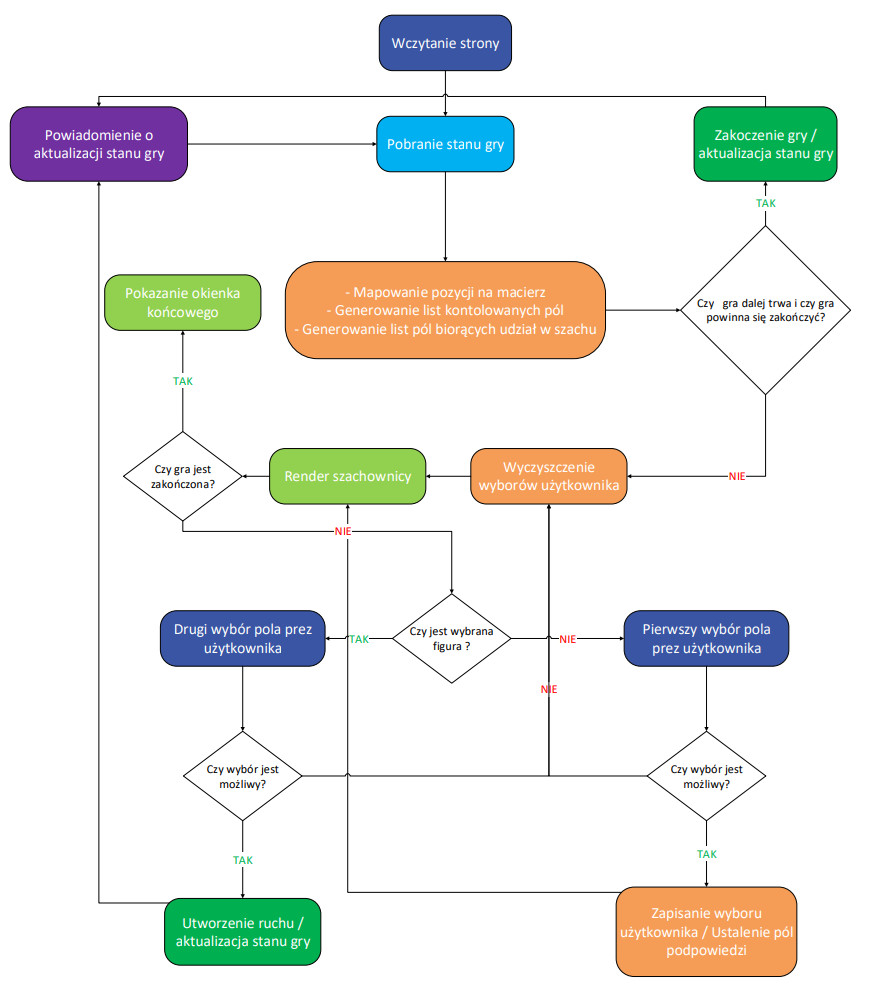
\includegraphics[width=1\textwidth]{images/diagram_gry.png}
    \caption{Diagram blokowy mechanizmu gry w szachy. Opracowany za pomocą aplikacji Viso.}
\end{figure}

\newpage

\noindent \textbf{Gra z silnikiem szachowym}\\
W przypadku gier z silnikiem szachowym mechanizmy rozgrywki są niemal identyczne jak w grach online. Kluczową różnicą jest jednak brak wykorzystania technologii SignalR, ponieważ w tym scenariuszu nie ma potrzeby powiadamiania drugiego użytkownika o wykonanych ruchach. Rozgrywka przebiega sekwencyjnie od początku do końca: po wykonaniu ruchu przez gracza aplikacja wysyła zapytanie do serwera, aby pobrać ruch zaproponowany przez silnik, a następnie wykonuje ruch jako odpowiedź przeciwnika.
\\\\
Środowisko niejako „symuluje” przeciwnika użytkownika, tworząc tymczasowe stany gry uzupełniane danymi wygenerowanymi przez silnik. Po otrzymaniu propozycji ruchu silnika wykonywana jest pełna procedura ruchu, z pominięciem sprawdzania jego legalności, ponieważ ten aspekt jest kontrolowany przez sam silnik szachowy.

\vspace{1cm}
\begin{figure}[h!]
    \centering
    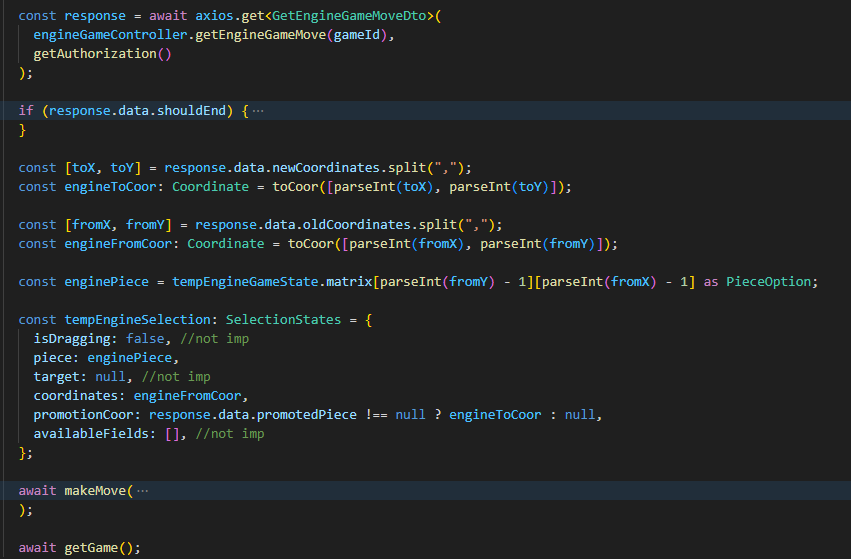
\includegraphics[width=1\textwidth]{images/ex_engine_move_sim.png}
    \caption{Fragment kodu: Symulacja ruchu zaproponowanego przez silnik.}
\end{figure}

\noindent
Jak widać na załączonym przykładzie program tworzy identyczny obiekt jaki jest wykorzystywany do śledzenia wyborów uzytkownika, z pominięciem nieistotnych wartości na następnie korzystając z tych samych funkcji jak w przypadku gry online, program wykonuje ruch podany przez AI. Takie podejście umożliwia ponowne wykorzystanie istniejących funkcji, aby nie powielać podobnej implementacji.

\newpage

\noindent
Poniżej przedstawiony został uproszony diagram blokowy przedstawiający działanie mechanizmu gry z przeciwnikiem komputerowym. Diagram zawiera tylko kluczowe zmiany, odnoszące się do komunikacji z silnikiem szachowym, natomiast pozostała funkcjonalność pozostaje identyczna, jak w przypadku mechanizmu gier online. pominięte zostały między innymi aspekty końca gry, czy rozdzielnia wyborów uzytkownika na opcje przed wybraniem figury i po wyborze, ponieważ są one identyczne w tym trybe gry offline.

\vspace{1cm}
\begin{figure}[h!]
    \centering
    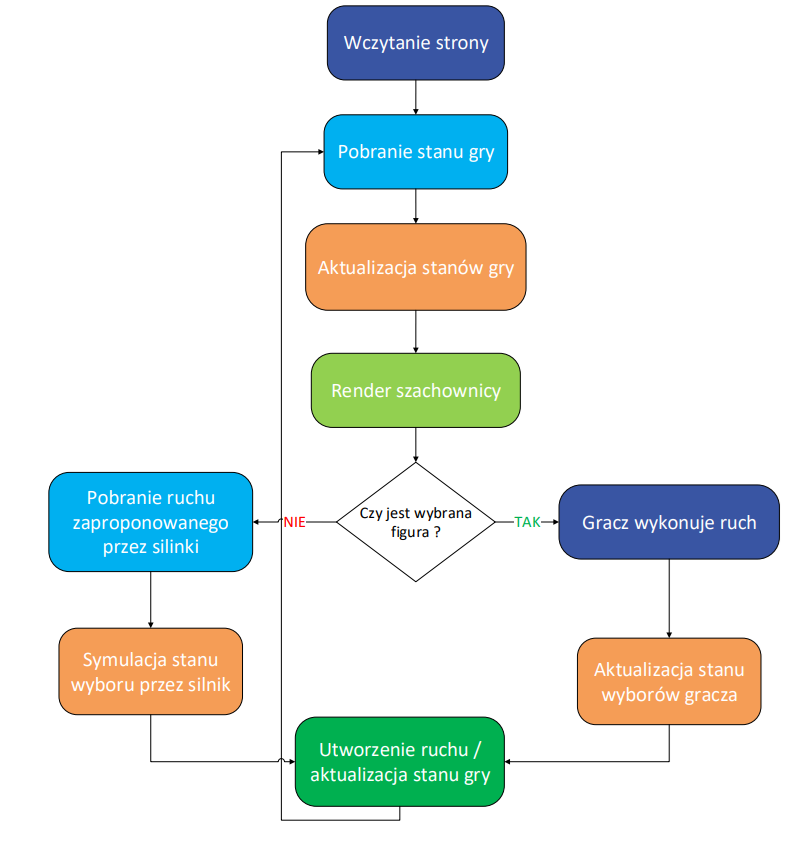
\includegraphics[width=1\textwidth]{images/diagram_enggry.png}
    \caption{Diagram blokowy mechanizmu gry z silnikiem. Opracowany za pomocą aplikacji Viso.}
\end{figure}

\newpage

\subsubsection{Kluczowe aspekty gry}

\noindent \textbf{Podstawowe oznaczenia}\\
Notacja Forsytha-Edwardsa (FEN) – zapis szachowy do określenia pozycji gry szachowej. Celem FEN jest podanie wszystkich niezbędnych informacji do ponownego rozpoczęcia gry od danej pozycji. FEN bazuje na systemie wymyślonym przez szkockiego dziennikarza Davida Forsytha. Jego system stał się popularny w XIX wieku; Steven J. Edwards rozwinął system by mógł działać z komputerami. FEN jest częścią Portable Game Notation dla szachów, dlatego że definiuje pozycje inne od początkowej.
\\\\
W formacie FEN figury szachowe są oznaczane literami, przy czym wielkie litery reprezentują figury białe, a małe litery figury czarne. Król oznaczany jest jako \textbf{K/k}, hetman jako \textbf{Q/q}, wieża jako \textbf{R/r}, goniec jako \textbf{B/b}, skoczek jako \textbf{N/n}, a pion jako \textbf{P/p}.
\\\\
Przy wszelkich obliczeniach związanych z ruchami figur oraz analizą innych aspektów gry szachowej wykorzystano system wektorów. Wektory te pozwalają precyzyjnie opisać ruchy każdej figury na szachownicy w formie zestawu współrzędnych. Poniżej przedstawiono dwa zestawy takowych wektorów.
\\\\
Wektory ruchów figur poruszających się liniowo i diagonalnie:

\[
\quad 
\begin{bmatrix}
    [0, 1] & [0, -1] & [1, 0] & [-1, 0] & [1, 1] & [1, -1] & [-1, 1] & [-1, -1]
\end{bmatrix}
\]

\noindent
Specyficzne wektory ruchów skoczka:

\[
\quad 
\begin{bmatrix}
    [1, 2] & [1, -2] & [-1, 2] & [-1, -2] & [2, 1] & [2, -1] & [-2, 1] & [-2, -1]
\end{bmatrix}
\]

\vspace{0.5cm}

\noindent \textbf{Oznaczenie ruchu}\\
Ruchy figurami są zapisywane w sposób precyzyjny i zrozumiały, zawierając wszystkie istotne informacje o wykonanej akcji. Składa się z kilku elementów:
\begin{itemize}
    \item \textbf{Symbol figury:} jeśli ruch dotyczy pionka, jest on pomijany.
    \item \textbf{Koordynaty pola początkowego:} współrzędne w formacie [A-H][1-8].
    \item \textbf{Znak bicia:} oznaczany jako znak „x”.
    \item \textbf{Koordynaty pola docelowego:} współrzędne w formacie [A-H][1-8].
    \item \textbf{Promocja pionka:} W przypadku promocji, dodaje się oznaczenie „=(symbol figury)”.
    \item \textbf{Szach lub mat:} oznaczone przez symbole: „+” szach oraz „\#”.
    \item \textbf{Czas wykonania ruchu:} podawany w przypadku gry z czasem.
\end{itemize}

\vspace{0.5cm}
\begin{figure}[h!]
    \centering
    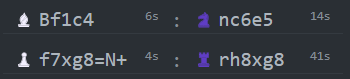
\includegraphics[width=0.5\textwidth]{images/imp_moves.png}
    \caption{Przykładowe ruchy wykonane podczas gry.}
\end{figure}

\newpage

\noindent \textbf{Pozycja FEN}\\
Pozycja FEN (Forsyth-Edwards Notation) to sposób zapisywania aktualnej sytuacji na szachownicy, który pozwala na jednoznaczne odtworzenie pozycji w dowolnym momencie gry. Zawiera wszystkie istotne informacje o rozmieszczeniu figur, kolorze gracza, który ma wykonać ruch, stanie roszady, liczbie ruchów od ostatniego bicia lub ruchu pionkiem, oraz liczbie pełnych ruchów.
\\\\
W kontekście aplikacji, zapis FEN jest wykorzystywany do przechowywania stanu gry w bazie danych. Dzięki temu możliwe jest zapisanie aktualnej pozycji w dowolnym momencie, a następnie jej odczytanie i przywrócenie, co pozwala na wznowienie gry lub analizę wcześniejszych stanów.


\begin{center}
    \texttt{rnbqkbnr/pppppppp/8/8/8/8/PPPPPPPP/RNBQKBNR w KQkq - 0 1}
\end{center}


\noindent
Przedstawioną powyżej przykładową pozycje można podzielić kolejno na części oznaczające:

\begin{itemize}
    \item Rozmieszczenie figur na szachownicy, z użyciem liter oraz liczb wskazujących puste pola.
    \item Kolor gracza, który ma wykonać ruch.
    \item Informacja o dostępności roszady dla obu graczy.
    \item Pozycja pionka, który może wykonać ruch en passant.
    \item Liczba ruchów od ostatniego bicia lub ruchu pionkiem.
    \item Liczba pełnych ruchów.
\end{itemize}

\noindent \textbf{Macierz szachownicy}\\
W pierwszej części zapisu pozycji FEN znajdują się informacje o rozmieszczeniu figur na szachownicy. Program przetwarza ten zapis, mapując go na macierz 8x8, co umożliwia łatwiejsze operowanie na koordynatach. Dzięki tej mapie, każdy element (pole) szachownicy może być odwoływany za pomocą indeksów, co ułatwia implementację ruchów, sprawdzanie stanu gry, a także operacje na poszczególnych figurach. Na przykład, każdemu polu szachownicy przypisane są współrzędne (x, y), gdzie x to numer kolumny (od A do H), a y to numer wiersza (od 1 do 8). Taki sposób reprezentacji umożliwia wygodną manipulację i analizowanie stanu gry.

\vspace{0.5cm}
\begin{figure}[h!]
    \centering
    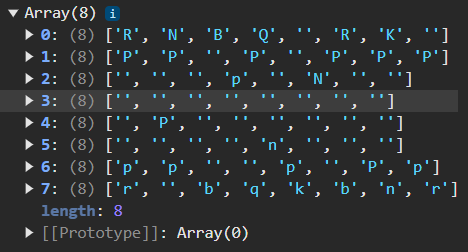
\includegraphics[width=0.7\textwidth]{images/ex_matrix.png}
    \caption{Przykładowa macierz pozycji gry.}
\end{figure}

\newpage

\noindent \textbf{Ruchy figur}\\
Proces wykonywania ruchów w programie opiera się na mechanizmie identyfikacji możliwych posunięć dla wybranej figury. Gdy użytkownik wybierze swoją figurę, uruchamiana jest metoda \textbf{find} z klasy \textbf{FindMoves}. Metoda ta analizuje aktualną pozycję na szachownicy i zwraca listę pól, na które dana figura może się legalnie przemieścić zgodnie z zasadami gry. Następnie, jeśli użytkownik wskaże jedno z pól podanych w tej liście, ruch zostaje wykonany, a szachownica zostaje zaktualizowana o nową pozycję figury. 
\\\\
Metoda \texttt{find} analizuje ruchy wybranej figury na podstawie jej symbolu i koordynat. Proces rozpoczyna się od sprawdzenia, czy figura znajduje się w sytuacji związania, co wpływa na ograniczenie jej możliwych ruchów. Następnie, w oparciu o mapę ruchów figur i identyfikację wybranego rodzaju figury, program generuje listę pól podpowiedzi. W przypadku wystąpienia związania, do funkcji generującej ruchy przekazywany jest dodatkowy parametr określający kierunek związania, co pozwala na zredukowanie możliwych ruchów. Na końcu, metoda weryfikuje, czy król gracza nie znajduje się w pozycji szacha. Jeśli tak, pola podpowiedzi zostają dodatkowo ograniczone.

\vspace{0.5cm}
\begin{figure}[h!]
    \centering
    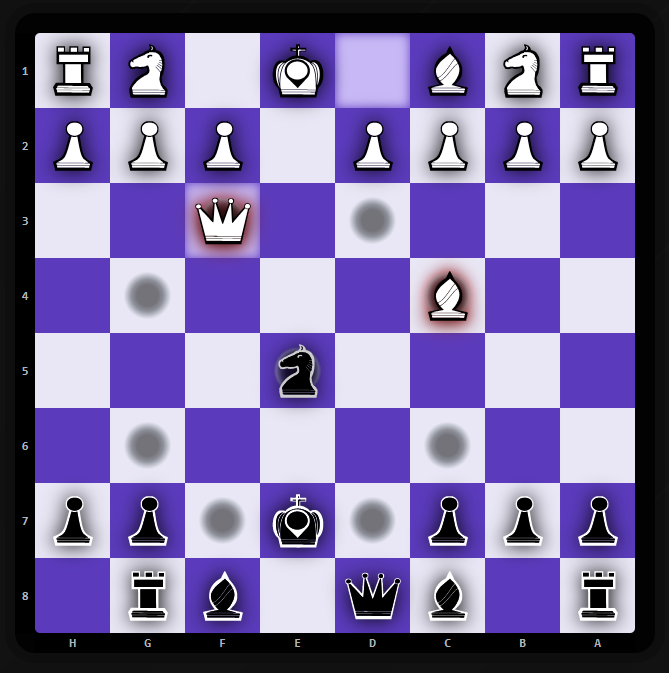
\includegraphics[width=0.5\textwidth]{images/imp_move_tips.png}
    \caption{Wizualizacja podpowiedzi ruchu.}
\end{figure}
\vspace{0.5cm}

\noindent
Po kliknięciu przez użytkownika na pole znajdujące się na liście pól podpowiedzi wywoływana jest funkcja \texttt{makeMove}. Funkcja ta tworzy oznaczenie ruchu w formacie FEN, które dokładnie opisuje wykonany ruch. Następnie aktualizowana jest zarówno bieżąca pozycja FEN, jak i macierz pozycji. Funkcja ta również aktualizuje stany gry, przechowujące dane niezbędne dla ruchów specjalnych. Po przeprowadzeniu tych aktualizacji następuje rozdzielenie logiki w zależności od trybu gry:

\begin{itemize}
    \item \textbf{Gra sieciowa:} Wywoływana jest metoda huba SignalR, w celu powiadomienia drugiego gracza o wykonanym ruchu.
    \item \textbf{Gra z silnikiem:} Następuje wywołanie API kontrolera odpowiedzialnego za interakcję z silnikiem szachowym.
\end{itemize}

\newpage

\noindent \textbf{Szach}\\
Jest to sytuacja w grze w szachy, w której król jednego z graczy znajduje się pod atakiem przeciwnika, co oznacza, że przeciwnik mógłby zbić króla w swoim kolejnym ruchu, gdyby nie został on obroniony. W odpowiedzi na szach gracz musi podjąć ruch eliminujący zagrożenie dla króla. Istnieją trzy możliwe sposoby na uniknięcie szacha:

\begin{itemize}
    \item Przesunięcie króla na pole, które nie jest zagrożone przez przeciwnika.
    \item Zasłonięcie króla inną figurą, jeśli zagrożenie pochodzi z linii działania.
    \item Zbicie atakującej figury, jeśli jest to możliwe.
\end{itemize}

\noindent
Nieodpowiedzenie na szach jest niedozwolone, ponieważ król nigdy nie może pozostawać na szachowanym polu. Jeśli gracz nie ma możliwości zneutralizowania szacha, partia kończy się matem.
\\\\
W projekcie sytuacja szachu została rozwiązana poprzez tworzenie dwóch par list. Pierwsza z nich obejmuje pola kontrolowane, czyli te, na które figury przeciwnika mogą wykonać bicie. Pola te są wykorzystywane do zapewnienia, że król nie może wejść na pole, na którym byłby zagrożony zbiciem, a także do sprawdzania, czy aktualnie znajduje się w szachu, jeśli stoi na takim polu.
\\\\
Druga para to listy pól biorących udział w szachu. Obejmują one pole zajmowane przez figurę szachującą oraz wszystkie pola, przez które szach jest „przekazywany” (na przykład w przypadku szachów liniowych, takich jak atak wieży, gońca czy hetmana). Pola te są wykorzystywane do ograniczenia możliwych ruchów innych figur, tak aby uniemożliwić wykonanie ruchu niezapewniającego zakończenia szachu. Dzięki temu mechanizmowi tylko ruchy ratujące króla są dopuszczalne w trakcie szachu, co w pełni odwzorowuje zasady gry w szachy.

\vspace{1cm}
\begin{minipage}[t]{0.45\textwidth} 
    \vspace{0pt} 
    \centering 
    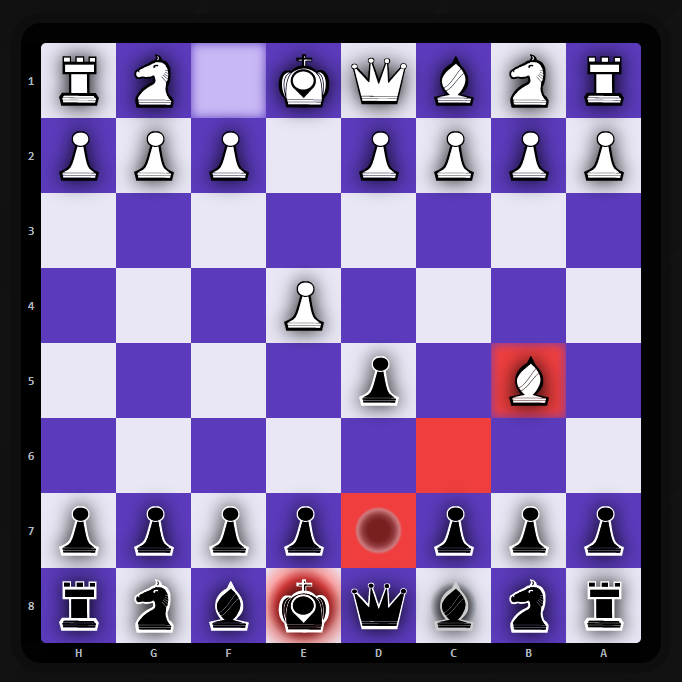
\includegraphics[width=\linewidth]{images/imp_front_check_areas.png} 
    Wizualizacja pól szachu.
\end{minipage} 
\hfill 
\begin{minipage}[t]{0.45\textwidth} 
    \vspace{0pt} 
    \centering 
    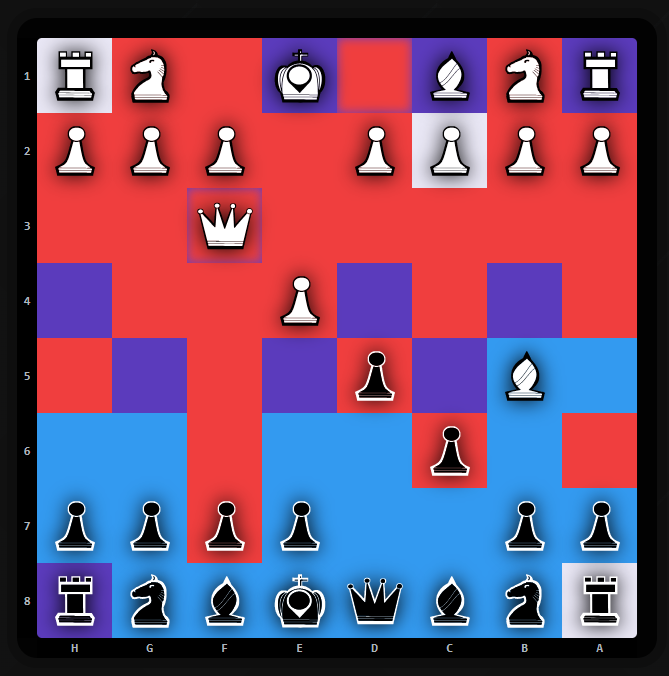
\includegraphics[width=\linewidth]{images/imp_front_controlled_areas.png} 
    Wizualizacja kontrolowanych pól.
\end{minipage}

\newpage

\noindent
Generowanie pól kontrolowanych i pól szachowych realizują funkcje: \texttt{generateControlledAreas} i \texttt{checkChecks}. Pierwsza iteruje przez macierz szachownicy, dodając do kontrolowanych pól wszystkie pozycje, na które figura może wykonać bicie, zgodnie z zasadami ruchu. Kontrolowane pola obejmują także zajęte przez figury, aby król nie mógł zbić bronionej figury. Funkcja \texttt{checkChecks} sprawdza, czy król jest w szachu, porównując jego pozycję z listą kontrolowanych pól przeciwnika. Dla figur szachujących dodaje do listy pola na linii szachu i pozycję szachującej figury.
\\\\

\noindent \textbf{Szach podwójny}\\
Jest to sytuacja, w której dwie figury biorą udział w szachu, a kierunki wykonywania szachow zawsze muszą być inne. Szach podwójny występuje wyłącznie w sytuacji szachu z odsłony, gdy dwie różne figury jednocześnie atakują króla przeciwnika. W grze szachowej może wystąpić jedynie szach zwykły lub szach podwójny – nie jest możliwe, aby więcej niż dwie figury jednocześnie szachowały króla. W praktyce istnieją następujące sytuacje, które mogą spowodować szach podwójny:

\begin{itemize}
    \item Goniec odsłania figure atakującą w liniach prostych.
    \item Wieża odsłania figure atakującą po diagonalach.
    \item Skoczek odsłania jakąkolwiek figure poruszającą się liniowo.
\end{itemize}

W programie mechanizm obsługi szachu podwójnego został zaimplementowany poprzez sprawdzanie liczby figur znajdujących się na polach biorących udział w szachu. Jeśli zostaną wykryte dwie figury szachujące króla, a wybrana przez gracza figura nie jest królem, pola podpowiedzi ruchów zostają wyzerowane. Wynika to z faktu, że w przypadku szachu podwójnego jedynym dozwolonym ruchem jest przesunięcie króla na bezpieczne pole.

\vspace{0.5cm}
\begin{figure}[h!]
    \centering
    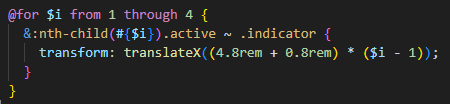
\includegraphics[width=0.5\textwidth]{images/imp_double_check.png}
    \caption{Przykład szachu podwójnego.}
\end{figure}

\newpage

\noindent \textbf{Mat i Pat}\\
W szachach mat oraz pat to dwie podstawowe sytuacje kończące grę. Mat oznacza, że król jednego z graczy jest w szachu i nie ma żadnych dostępnych ruchów, które mogłyby go uratować. Gra kończy się zwycięstwem przeciwnika. Pat, z kolei, ma miejsce wtedy, gdy gracz nie jest w szachu, ale nie ma żadnego legalnego ruchu, który mógłby wykonać. W takiej sytuacji gra kończy się remisem.
\\\\
W implementacji gry, te dwa scenariusze są rozwiązywane poprzez sprawdzanie dostępnych ruchów dla gracza, który jest aktualnie w turze. Gdy gracz próbuje wykonać ruch, najpierw sprawdzane jest, czy istnieje jakikolwiek możliwy ruch. Jeśli gracz nie ma żadnego dostępnego ruchu, program przechodzi do dalszej analizy.
\\\\
Jeśli po sprawdzeniu okazuje się, że gracz nie ma żadnych możliwych ruchów, następnie sprawdzane jest, czy jego król znajduje się w szachu. Jeśli król jest w szachu, oznacza to, że gra kończy się matem, a zwycięzcą zostaje przeciwnik. W przeciwnym przypadku, jeżeli gracz nie ma ruchu, ale jego król nie jest w szachu, oznacza to, że mamy do czynienia z patem, a gra kończy się remisem.
\\\\
Za cały opisany mechanizm odpowiada specjalnie dedykowana funkcja \texttt{checkIfAnyMoveExists}. Używa ona macierzy pozycji, aby sprawdzić każde pole na szachownicy oraz korzysta z mechanizmu klasy do znajdywania podpowiedzi, aby okreslic czy figura moze wykonac ruch. W ten sposób nie ma konieczności tworzenia całej implantacji sprawdzania każdej figury, sama funkcja kończy swoje działanie po natrafieniu na pierwszego pionka, który może wykonać ruch.

\vspace{0.5cm}
\begin{figure}[h!]
    \centering
    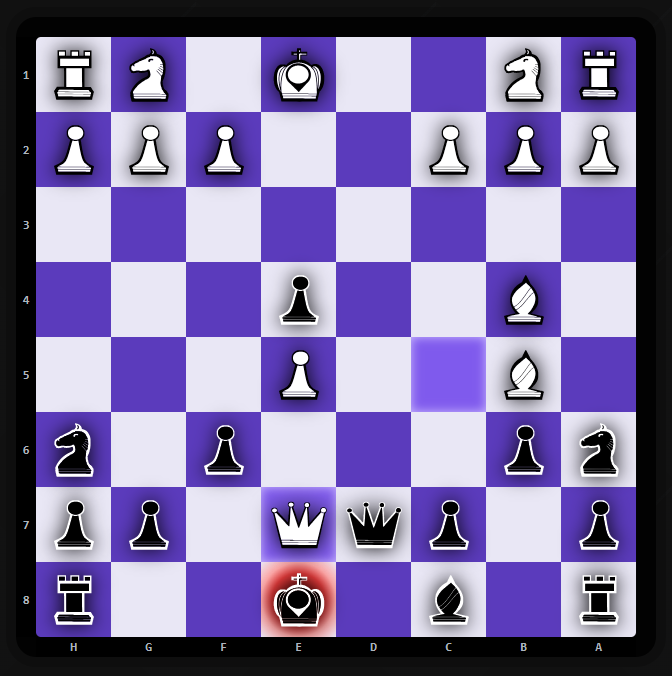
\includegraphics[width=0.5\textwidth]{images/imp_front_checkmate.png}
    \caption{Przykładu zakończenia gry matem.}
\end{figure}
\vspace{0.5cm}

\noindent
Tego rodzaju mechanizm pozwala na prawidłowe rozpoznawanie zakończenia gry w sytuacjach, kiedy gracz nie ma już możliwości wykonania ruchu, a także zapewnia zgodność z obowiązującymi zasadami gry.

\newpage

\noindent \textbf{Pin (Przypięcie)}\\
W szachach ruchy dzielą się na liniowe i nieliniowe. Liniowe obejmują ruchy prostoliniowe oraz diagonalne. Figury poruszające się liniowo to wieża, goniec i hetman. Nieliniowe ruchy charakteryzują się bardziej złożonymi trajektoriami, jak w przypadku skoczka.
\\\\
W implementacji gry mechanizm wykrywania pina opiera się na analizie linii prostych i diagonalnych między królem a wybraną figurą. Sprawdzane jest, czy w tej samej linii znajduje się figura przeciwnika, zdolna do wykonania ruchu liniowego (wieża, goniec lub hetman). Jeśli taka sytuacja występuje, to ruchy wybranej figury są ograniczone do kierunku pina – figura może się poruszać jedynie w linii między królem a figurą przeciwnika, o ile jej natura pozwala na ruch w tym kierunku.
\\\\
Mechanizm pina może być zastosowany wyłącznie przez figury poruszające się liniowo: wieżę, gońca i hetmana. Ich zdolność do kontroli dużej liczby pól sprawia, że pin jest jednym z kluczowych narzędzi taktycznych w szachach, zarówno w ataku, jak i w obronie. Implementacja tego mechanizmu zapewnia zgodność z regułami gry, jednocześnie dodając istotną warstwę realizmu i taktyki do systemu.

\vspace{1cm}
\begin{minipage}[t]{0.45\textwidth} 
    \vspace{0pt} 
    \centering 
    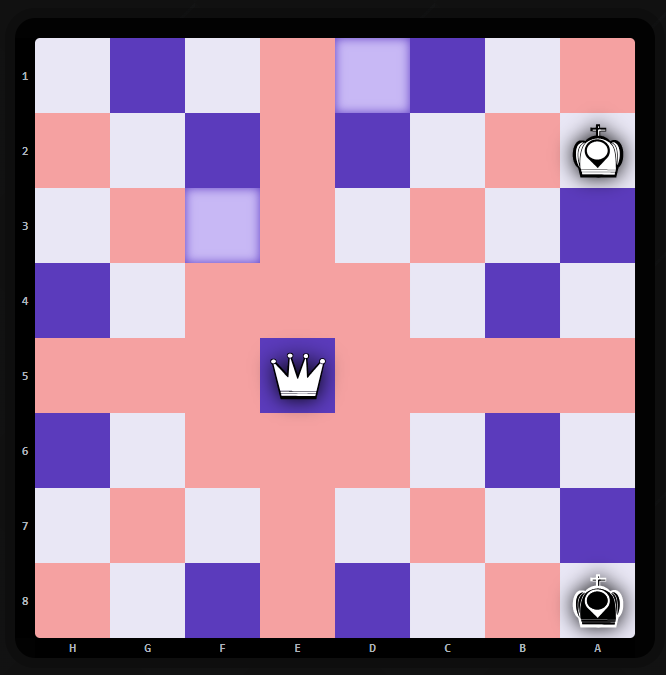
\includegraphics[width=\linewidth]{images/imp_front_linear.png} 
    Wizualizacja ruchów liniowych na przykładzie ruchów hetmana.
\end{minipage} 
\hfill 
\begin{minipage}[t]{0.45\textwidth} 
    \vspace{0pt} 
    \centering 
    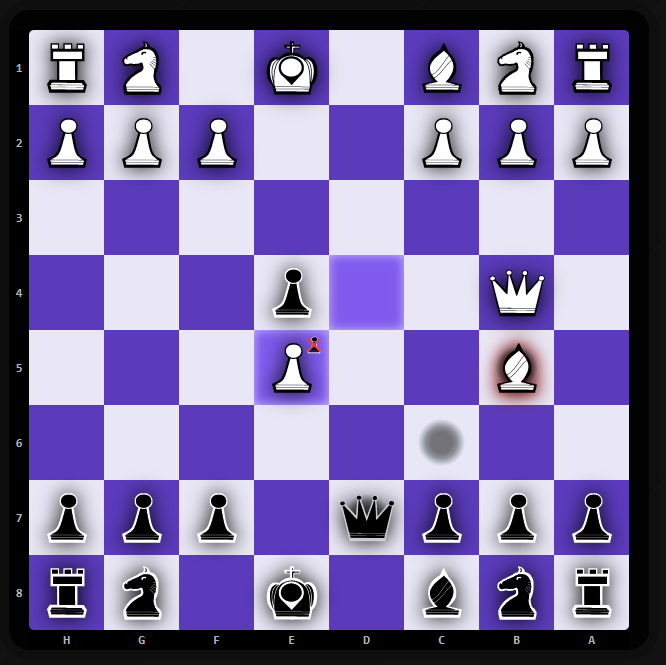
\includegraphics[width=\linewidth]{images/imp_front_pin.png} 
    Wizualizacja przykładowego pinu na hetmanie.
\end{minipage}
\vspace{1cm}

\noindent
Ponadto, w kontekście końca gry, piny odgrywają istotną rolę w decydowaniu, czy gra powinna się zakończyć. Mogą one ograniczać dostępne ruchy i zmuszać gracza do wykonania ruchu, który może prowadzić do matu lub patu. Gdy pionki, figury lub król zostają "przypięte", ich możliwości manewru są ograniczone, co znacząco wpływa na dalszy przebieg rozgrywki. Dodatkowo, jeśli przypięta figura nie może się poruszyć, może to prowadzić do sytuacji, w której gracz nie ma wystarczającej ilości ruchów do obrony, co przyczynia się do ostatecznego zwycięstwa.

\newpage

\noindent \textbf{Ruchy specjalne}\\
Ruchy specjalne w szachach, są przetwarzane za pomocą zapisanych specjalnych stanów w bazie danych. Na przykład, system przechowuje informacje o tym, czy roszada może zostać wykonana, bazując na wcześniejszych ruchach króla i wieży oraz innych warunkach, takich jak brak przeszkód na drodze. Ponadto, wykorzystywane są stałe wartości, takie jak pozycja pionka (tzw. ranga), które decydują o tym, kiedy dochodzi do promocji pionka, czy też kiedy pionek ma możliwość poruszenia się o dwa pola do przodu.

\vspace{1cm}
\begin{minipage}[t]{0.6\textwidth} 
    \vspace{0pt} 
    \raggedright 
    \textbf{Roszada}\\
    Roszada jest specjalnym ruchem, który polega na jednoczesnym przesunięciu króla i wieży. Aby ten ruch był możliwy, muszą być spełnione określone warunki, takie jak brak wcześniejszych ruchów króla i wieży oraz brak przeszkód między nimi. Dodatkowo, król nie może być w szachu ani przechodzić przez pole, które jest zagrożone.
\end{minipage} 
\hfill 
\begin{minipage}[t]{0.3\textwidth} 
    \vspace{0pt} 
    \centering 
    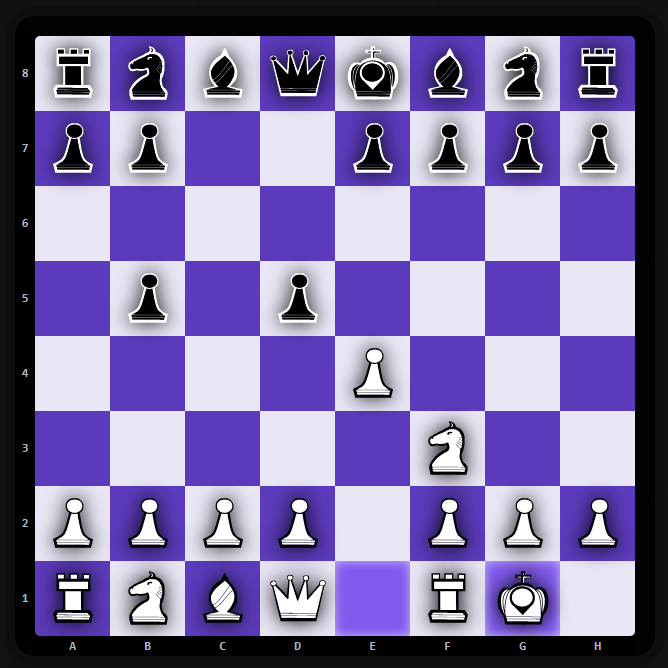
\includegraphics[width=\linewidth]{images/imp_front_castling.png} 
\end{minipage}
\vspace{1cm}
\begin{minipage}[t]{0.3\textwidth} 
    \vspace{0pt} 
    \centering 
    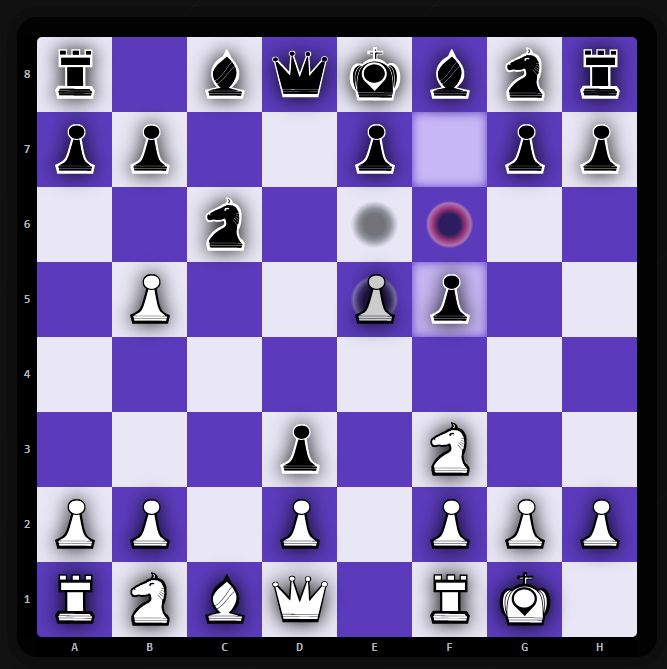
\includegraphics[width=\linewidth]{images/imp_front_enpassant.png} 
\end{minipage} 
\hfill 
\begin{minipage}[t]{0.6\textwidth} 
    \vspace{0pt} 
    \raggedright 
    \textbf{Bicie w przelocie}\\
    Bicie w przelocie jest specyficznym przypadkiem, który może wystąpić, gdy pionek przeciwnika poruszy się o dwa pola do przodu, a nasz pionek znajduje się na sąsiednim polu. W takim przypadku nasz pionek może zbić pionka przeciwnika, jakby poruszył się tylko o jedno pole. System zapisuje koordynat, na którym może paść to bicie w stanie gry.
\end{minipage}
\vspace{1cm}
\begin{minipage}[t]{0.6\textwidth} 
    \vspace{0pt} 
    \raggedright 
    \textbf{Promocja pionka}\\
    Promocja pionka ma miejsce, gdy pionek dotrze do ostatniej linii planszy. Wtedy gracz ma możliwość wymiany pionka na inną figurę, najczęściej na hetmana, ale także na wieżę, gońca lub skoczka. Promocja jest obsługiwana przez system na podstawie pozycji pionka na planszy, czyli tzw. rangi, która determinuje moment jej wykonania.
\end{minipage} 
\hfill 
\begin{minipage}[t]{0.3\textwidth} 
    \vspace{0pt} 
    \centering 
    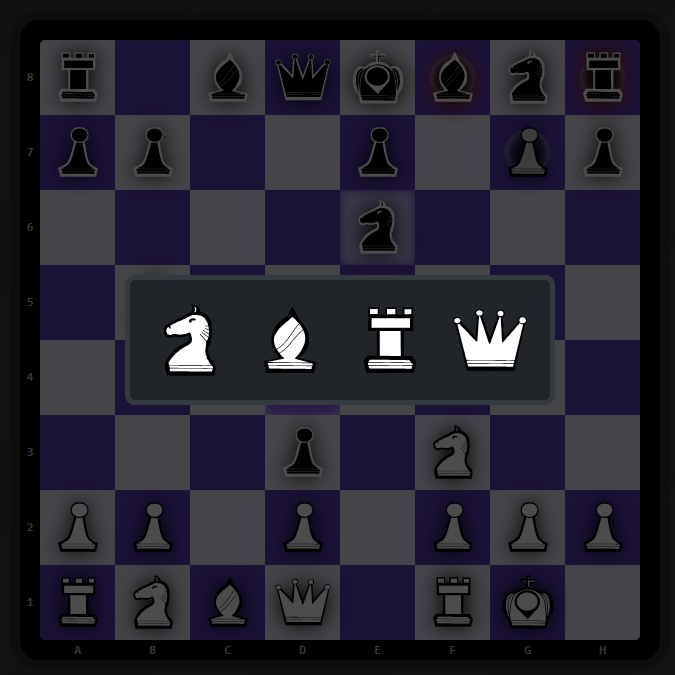
\includegraphics[width=\linewidth]{images/imp_front_promotion.png} 
\end{minipage}

\newpage

\noindent \textbf{Pozostałe zasady końca gry}\\
W szachach istnieje kilka innych zasad, które mogą prowadzić do zakończenia gry przed standardowym zwycięstwem lub remisem. Oprócz klasycznego szacha-mata, są to zasady, które umożliwiają ogłoszenie remisu, nawet jeśli nie ma bezpośredniego zagrożenia dla króla. System ten wymaga od aplikacji precyzyjnego śledzenia przebiegu gry oraz różnych warunków, które mogą prowadzić do remisu. Oto szczegóły niektórych z tych zasad:

\begin{itemize}
    \item \textbf{Zasada trzykrotnego powtórzenia pozycji}\\
    Zasada ta pozwala ogłosić remis, jeśli ta sama pozycja na szachownicy wystąpiła trzykrotnie podczas gry, pod warunkiem, że pozycje te miały tę samą możliwość wykonania ruchu. W programie realizuje się to przez zapisanie wszystkich wykonanych ruchów oraz ich stanów w bazie danych. Program porównuje zapisaną historię i sprawdza, czy dana pozycja pojawiła się już co najmniej trzykrotnie. Jeśli tak, gra kończy się remisem.
    \item \textbf{Zasada 50 ruchów}\\
    Zasada 50 ruchów oznacza, że jeśli przez 50 kolejnych ruchów nie została wykonana żadna akcja, taka jak ruch pionka lub bicie figury, to gra kończy się remisem. W aplikacji ten stan jest śledzony za pomocą specjalnej zmiennej, która liczy tzw. "halfmove" (połowa ruchu). Zwiększa się ona o 1 za każdym razem, gdy nie został wykonany ruch pionka lub nie doszło do bicia. Jeśli liczba ta osiągnie 50, program uznaje, że zasada została spełniona i gra kończy się remisem. Jeśli w tym czasie wykonany zostanie ruch pionka lub dojdzie do bicia, licznik jest zerowany.
    \item \textbf{Niewystarczający ilość materiału}\\
    Jeśli na szachownicy nie ma wystarczającej ilości figur, aby móc wykonać mat, gra kończy się remisem. Na przykład, jeśli jeden z graczy ma tylko króla, a drugi gracz ma jedynie króla i jakąkolwiek inną figurę, nie będzie już możliwe zrealizowanie matu. W takim przypadku aplikacja analizuje całą planszę i sprawdza, czy występuje wystarczający materiał do wykonania matu. Jeżeli materiał jest niewystarczający, program ogłasza remis.
\end{itemize}

\noindent \textbf{Upłynięcie czasu}\\
W przypadku gry z czasem, aplikacja śledzi czas pozostały dla obu graczy i przechowuje te informacje w bazie danych. Czas jest odliczany dla każdego gracza indywidualnie, a po wykonaniu ruchu przez jednego z graczy, zegar zostaje zaktualizowany. Czas jest inkrementowany na podstawie zadanego interwału, który może być ustalony na początku gry. Kiedy jeden gracz wykonuje ruch, czas zostaje zaktualizowany o odpowiedni inkrement, a zegar drugiego gracza zaczyna odliczać swój czas. Cały proces jest realizowany poprzez zapisywanie stanu czasu w bazie danych oraz bieżące odliczanie dla aktywnego gracza. Jeśli czas któregokolwiek z graczy dobiegnie końca, gra automatycznie kończy się, a przegrany zostaje ogłoszony przegranym z powodu przekroczenia czasu. Tego typu funkcjonalność jest szczególnie przydatna w trybach szybkich gier, gdzie gracze mają określoną ilość czasu na wykonanie swoich ruchów.

\newpage

\subsubsection{Stylizacja komponetów}

\noindent
Każdy komponent w projekcie posiada własny folder, w którym znajduje się dedykowany plik stylów o nazwie \texttt{.module.scss}. Dzięki temu stylizacja jest zorganizowana i łatwa do zarządzania. W przypadkach, gdy kilka komponentów o identycznej strukturze i umiejscowieniu wymaga podobnej stylizacji, ale różni się funkcjonalnością, korzystają one ze wspólnego pliku \texttt{.module.scss}. W takim pliku definiowane są style dla każdego z tych komponentów.
\\\\
Mechanizm stylizacji polega na imporcie klas z pliku \texttt{.module.scss} do pliku komponentu. Klasy te są następnie wykorzystywane jako zmienne, co pozwala na dynamiczne ich przypisywanie w zależności od logiki działania komponentu.
\\\\
Dodatkowo w folderze \texttt{shared} znajduje się plik \texttt{shared.scss}, który pełni funkcję centralnego miejsca dla zmiennych i mixinów współdzielonych przez różne komponenty. Plik ten gromadzi zadeklarowane wartości wspólne dla stylów, takie jak kolory, rozmiary czy powtarzające się schematy. Każdy plik stylów komponentów importuje go za pomocą deklaracji:

\begin{verbatim} @use "../shared/styles/shared.scss" as *; \end{verbatim}

Dzięki temu wszystkie zmienne i mixiny są dostępne w stylach poszczególnych komponentów, co pozwala na spójność oraz łatwą aktualizację stylów w całym projekcie.
\\\\
Mixiny są jednym z najważniejszych narzędzi oferowanych przez SCSS, umożliwiającym tworzenie wielokrotnego użytku fragmentów kodu CSS. Dzięki nim można zdefiniować zestawy stylów z opcjonalnymi parametrami, które można stosować w różnych miejscach projektu. To podejście znacznie przyspiesza pracę, ponieważ eliminuje konieczność ręcznego powielania kodu i pozwala na łatwą modyfikację stylów w jednym miejscu. Szczególnie dobrze sprawdzają się przy definiowaniu powtarzalnych wzorców, takich jak style przycisków, cieni, animacji czy układów. Ich wykorzystanie zwiększa spójność projektu i ułatwia utrzymanie kodu, co jest kluczowe w przypadku dużych aplikacji z wieloma komponentami. Dzięki mixinom stylizacja staje się bardziej modułowa, elastyczna i łatwa do skalowania.
\\\\
Dodatkowo, jak przedstawiono na zdjęciu poniżej, SCSS umożliwia wykorzystanie konstrukcji sterujących , które pozwalają na dynamiczne generowanie stylów. Dzięki nim można w prosty sposób tworzyć bardziej elastyczne i zautomatyzowane reguły stylizacji, co znacząco usprawnia pracę nad projektem.

\vspace{0.5cm}
\begin{figure}[h!]
    \centering
    \includegraphics[width=0.7\textwidth]{images/ex_loop_scss.png}
    \caption{Fragment kodu: Dynamiczne tworzenie stylów.}
\end{figure}
\vspace{0.5cm}

Na zakończenie warto podkreślić, że niemal każdy plik stylizacji komponentu zawiera znaczniki odpowiadające za obsługę mniejszych urządzeń. Dzięki temu strona została zoptymalizowana pod kątem responsywności, co pozwala na jej wygodne użytkowanie na dowolnym rodzaju urządzenia.


\newpage

\subsubsection{Wykorzystane biblioteki}

\begin{itemize} 
    \item \textbf{react} i \textbf{react-dom}: React to biblioteka do tworzenia dynamicznych komponentów UI, a react-dom pozwala na renderowanie tych komponentów w DOM, integrując aplikację React z przeglądarką. 
    \item \textbf{typescript}: Typowanie statyczne dla JavaScript, które pomaga unikać błędów w kodzie oraz poprawia jego skalowalność.
    \item \textbf{@microsoft/signalr}: Biblioteka umożliwiająca komunikację w czasie rzeczywistym między aplikacjami frontendowymi a serwerem. Jest kluczowa do implementacji funkcji czatu, powiadomień lub innych aplikacji wymagających bieżącej wymiany danych w czasie rzeczywistym.
    \item \textbf{axios} i \textbf{msw}: Axios to klient HTTP do wysyłania zapytań do API, a MSW umożliwia mockowanie tych zapytań w trakcie rozwoju lub testowania aplikacji bez potrzeby aktywnego backendu. 
    \item \textbf{history} i \textbf{react-router-dom}: History umożliwia zarządzanie historią przeglądarki, a react-router-dom korzysta z tej biblioteki do obsługi routingu i nawigacji w aplikacjach SPA. 
    \item \textbf{jsonwebtoken} i \textbf{jwt-decode}: Biblioteki związane z uwierzytelnianiem. `jsonwebtoken` służy do tworzenia i weryfikacji tokenów JWT, które są używane do autoryzacji użytkowników, a `jwt-decode` umożliwia dekodowanie tych tokenów, pozwalając na ekstrakcję danych, takich jak dane użytkownika lub czas wygaśnięcia tokenu.
    \item \textbf{guid-typescript} i \textbf{uuid}: Obie biblioteki umożliwiają generowanie unikalnych identyfikatorów, które mogą być używane w aplikacjach do identyfikowania elementów, sesji lub użytkowników. 
    \item \textbf{vite} i \textbf{vitest}: Vite to bundler i serwer deweloperski, który wspiera nowoczesne technologie, a vitest to framework testowy zoptymalizowany pod kątem ekosystemu Vite, umożliwiający szybkie uruchamianie testów jednostkowych. 
    \item \textbf{@testing-library/dom} i \textbf{@testing-library/react}: Biblioteki do testowania DOM i komponentów React, umożliwiające tworzenie testów jednostkowych i integracyjnych w aplikacjach frontendowych. 
    \item \textbf{eslint} i \textbf{@eslint/js}: Narzędzia do statycznej analizy kodu w celu zapewnienia jakości i spójności kodu JavaScript, zgodnie z określonymi zasadami. 
    \item \textbf{stylelint}: Narzędzie do analizy jakości CSS i SCSS, zapewniające porządek w kodzie stylów. 
    \item \textbf{sass} i \textbf{scss}: Obie biblioteki to preprocesory CSS, gdzie SCSS jest bardziej zbliżoną do standardowego CSS wersją SASS. Używa się ich do organizowania i modularnego pisania stylów. 
\end{itemize}

\newpage

\section{Instrukcja obsługi}
\subsection{Strona startowa}
Strona tytułowa aplikacji do gry w szachy została zaprojektowana jako intuicyjny i funkcjonalny punkt startowy dla użytkowników. Umieszczono na niej wszystkie kluczowe elementy, które pozwalają na łatwe rozpoczęcie korzystania z platformy. W górnej części strony znajdują się przyciski umożliwiające logowanie oraz rejestrację, co pozwala zarówno nowym użytkownikom, jak i tym posiadającym konto na szybki dostęp do zasobów aplikacji.
\\\\
Całość zaprojektowano w sposób przejrzysty i estetyczny, aby zapewnić pozytywne pierwsze wrażenie oraz łatwość w poruszaniu się po stronie. Strona tytułowa pełni rolę wizytówki aplikacji, jednocześnie oferując dostęp do najważniejszych zasobów i funkcji.

\vspace{0.5cm}
\begin{figure}[h!]
    \centering
    \includegraphics[width=1\textwidth]{images/ins_hero.png}
    \caption{Instrukcja: Widok strony startowej.}
\end{figure}
\vspace{0.5cm}

\noindent
Stronę startową podzielono na kilka sekcji, mających na celu wprowadzenie użytkownika do platformy oraz prezentację kluczowych aspektów aplikacji. Każda z tych sekcji została zaprojektowana tak, aby użytkownik mógł łatwo zrozumieć funkcjonalności oferowane przez aplikację i szybko rozpocząć korzystanie z niej.

\newpage

\begin{minipage}[t]{0.3\textwidth} 
    \vspace{0pt} 
    \centering 
    \includegraphics[width=\linewidth]{images/ins_home.png} 
\end{minipage} 
\hfill 
\begin{minipage}[t]{0.6\textwidth} 
    \vspace{0pt} 
    \raggedright 
    Pierwsza sekcja strony startowej zawiera krótki wstęp o aplikacji, który przedstawia jej główne założenia i funkcjonalności. Znajdują się tu również przyciski umożliwiające szybkie przejście do logowania lub rejestracji, ułatwiając rozpoczęcie korzystania z platformy.
\end{minipage}

\vspace{1cm}

\begin{minipage}[t]{0.6\textwidth} 
    \vspace{0pt} 
    \raggedright 
    Druga sekcja, umożliwia szybki dostęp do funkcji rozgrywki. Znajdują się tutaj przyciski pozwalające na szybkie wyszukiwanie gier online z innymi graczami oraz rozpoczęcie gry offline przeciwko komputerowi.
\end{minipage}
\hfill 
\begin{minipage}[t]{0.3\textwidth} 
    \vspace{0pt} 
    \centering 
    \includegraphics[width=\linewidth]{images/ins_play.png} 
\end{minipage} 

\vspace{1cm}

\begin{minipage}[t]{0.3\textwidth} 
    \vspace{0pt} 
    \centering 
    \includegraphics[width=\linewidth]{images/ins_learn.png} 
\end{minipage} 
\hfill 
\begin{minipage}[t]{0.6\textwidth} 
    \vspace{0pt} 
    \raggedright 
    Trzecia sekcja, zawiera opisy kluczowych aspektów aplikacji, takich jak jej funkcje edukacyjne i możliwości rozwoju w grze. Na końcu tej sekcji znajduje się przycisk powrotu na górę, który umożliwia użytkownikowi szybki powrót, aby ponownie przejść do logowania lub rejestracji.
\end{minipage}

\vspace{1cm}

\begin{minipage}[t]{0.6\textwidth} 
    \vspace{0pt} 
    \raggedright 
    Czwarta sekcja, FAQ (Najczęściej Zadawane Pytania), zawiera odpowiedzi na pytania dotyczące dwóch głównych obszarów: zakładania i zarządzania kontem użytkownika oraz zasad i funkcji związanych z rozgrywkami.
\end{minipage}
\hfill 
\begin{minipage}[t]{0.3\textwidth} 
    \vspace{0pt} 
    \centering 
    \includegraphics[width=\linewidth]{images/ins_faq.png} 
\end{minipage} 

\vspace{1cm}

\begin{minipage}[t]{0.3\textwidth} 
    \vspace{0pt} 
    \centering 
    \includegraphics[width=\linewidth]{images/ins_footer.png} 
\end{minipage} 
\hfill 
\begin{minipage}[t]{0.6\textwidth} 
    \vspace{0pt} 
    \raggedright 
    Ostatnia sekcja, Footer, zawiera informacje kontaktowe oraz odnośniki do mediów społecznościowych. Umożliwia użytkownikom łatwy dostęp do danych kontaktowych oraz śledzenia aplikacji na platformach społecznościowych.
\end{minipage}

\vspace{1cm}

\begin{minipage}[t]{0.6\textwidth} 
    \vspace{0pt} 
    \raggedright 
    Oprócz strony startowej, aplikacja zawiera również osobną stronę About, która poświęcona jest wyjaśnieniu podstawowych pojęć oraz dostarcza użytkownikom ważne informacje dotyczące korzystania z platformy. Strona ta zawiera szczegółowe zapisy dotyczące warunków korzystania z aplikacji oraz polityki prywatności, które użytkownicy powinni poznać przed rozpoczęciem korzystania z platformy.
\end{minipage}
\hfill 
\begin{minipage}[t]{0.3\textwidth} 
    \vspace{0pt} 
    \centering 
    \includegraphics[width=\linewidth]{images/ins_about.png} 
\end{minipage} 

\newpage

\subsection{Strona rejestracji}
Strona rejestracji w aplikacji łączy w sobie wszystkie kluczowe funkcje niezbędne do zarządzania kontem użytkownika. Pozwala na założenie nowego profilu, zalogowanie się na istniejące konto, odzyskanie dostępu w przypadku utraty hasła oraz potwierdzenie adresu e-mail jako element weryfikacji konta. Wszystkie te opcje zostały zaprojektowane w sposób intuicyjny i łatwy w obsłudze, aby zapewnić jak najlepsze doświadczenie użytkownika.
\\\\
Proces rejestracji umożliwia szybkie i bezproblemowe utworzenie konta. Po podaniu podstawowych danych, takich jak adres e-mail, nawa użytkownika oraz hasło, użytkownik otrzymuje wiadomość e-mail z linkiem aktywacyjnym, który potwierdza poprawność podanych informacji i zabezpiecza konto przed nieautoryzowanym dostępem. Logowanie do istniejącego konta odbywa się poprzez wprowadzenie e-maila lub nazwy uzytkownika i hasła.
\\\\
W przypadku zapomnianego hasła, strona oferuje funkcję jego odzyskania. Po podaniu adresu e-mail użytkownik otrzymuje szczegółowe instrukcje dotyczące resetowania hasła, co pozwala w bezpieczny sposób odzyskać dostęp do konta. Proces jest prosty i zabezpieczony dodatkowymi krokami weryfikacyjnymi.

\vspace{0.5cm}
\begin{figure}[h!]
    \centering
    \includegraphics[width=1\textwidth]{images/ins_reg.png}
    \caption{Instrukcja: Widok strony rejestracji użytkowników.}
\end{figure}
\vspace{0.5cm}

\noindent
Strona rejestracji jest zaprojektowana z myślą o czytelności i łatwości obsługi, dzięki czemu użytkownicy mogą bez przeszkód korzystać z jej funkcji niezależnie od poziomu zaawansowania. Wszystkie kroki są jasno opisane, a interfejs dostosowano do potrzeb zarówno nowych, jak i stałych użytkowników aplikacji.

\newpage

\subsection{Weryfikacja konta}

\begin{minipage}[t]{0.55\textwidth} 
    \vspace{0pt} 
    \raggedright 
    Weryfikacja konta to jeden z kluczowych etapów rejestracji, mający na celu zapewnienie bezpieczeństwa danych użytkowników oraz ochronę przed nieuprawnionym dostępem. Po zakończeniu procesu rejestracji aplikacja automatycznie generuje wiadomość e-mail, która zawiera wszystkie informacje niezbędne do ukończenia weryfikacji. System weryfikacyjny nie tylko wspiera proces zakładania konta, ale również jest wykorzystywany przy odzyskiwaniu hasła, co zapewnia spójność działania i zwiększa bezpieczeństwo użytkowników. 
\end{minipage} 
\hfill 
\begin{minipage}[t]{0.35\textwidth} 
    \vspace{0pt} 
    \centering 
    \includegraphics[width=\linewidth]{images/ins_min_ver.png} 
    Okno weryfikacji adresu email.
\end{minipage}

\vspace{1cm}

\begin{minipage}[t]{0.35\textwidth} 
    \vspace{0pt} 
    \centering 
    \includegraphics[width=\linewidth]{images/ins_min_mail.png} 
    Otrzymany email z kodem weryfikacyjnym.
\end{minipage} 
\hfill 
\begin{minipage}[t]{0.55\textwidth} 
    \vspace{0pt} 
    \raggedright 
    Wiadomość e-mail, zatytułowana "Hello from BRN Chess", zawiera przyjazne powitanie, a także unikalny kod weryfikacyjny przypisany do konkretnego konta użytkownika. Treść e-maila została zaprojektowana tak, aby była czytelna i estetyczna, co pozwala na szybkie odnalezienie wymaganych informacji. Kod weryfikacyjny, przedstawiony w formie wyróżnionego tekstu, należy skopiować i wkleić w dedykowane pole tekstowe w oknie weryfikacji w aplikacji. Po wprowadzeniu kodu i jego zatwierdzeniu konto zostaje w pełni aktywowane, a użytkownik może rozpocząć korzystanie z platformy. 
\end{minipage}

\vspace{1cm}

\noindent
Cały proces został opracowany z myślą o wygodzie użytkownika. Okno weryfikacyjne w aplikacji jest intuicyjne, zawiera czytelne instrukcje oraz widoczne przyciski umożliwiające wprowadzenie kodu. Dodatkowo w przypadku problemów, takich jak brak dostarczenia wiadomości e-mail, aplikacja oferuje możliwość ponownego wysłania kodu weryfikacyjnego za pomocą jednego kliknięcia.

\newpage

\subsection{Strona główna}
Strona główna aplikacji szachowej została zaprojektowana z myślą o intuicyjnej nawigacji i szybkim dostępie do kluczowych funkcji, aby zapewnić użytkownikom wygodę i efektywność. Po prawej stronie ekranu znajduje się pasek nawigacji, który umożliwia łatwe przechodzenie między różnymi stronami aplikacji, zapewniając dostęp do wszystkich istotnych sekcji. Pasek został umieszczony w widocznym miejscu, dzięki czemu poruszanie się po aplikacji jest szybkie i płynne.
\\\\
Obok paska nawigacji umieszczono główne przyciski, które prowadzą do najważniejszych funkcji aplikacji. Każdy z nich odpowiada za inną czynność:

\begin{itemize}
    \item \textbf{Gra online:} umożliwia rozpoczęcie partii z innym graczem przez internet.
    \item \textbf{Gra z komputerem:} pozwala zmierzyć się z silnikiem szachowym.
    \item \textbf{Gra ze znajomymi:} umożliwia zapraszanie znajomych do wspólnej gry.
    \item \textbf{Wgląd w gry użytkownika:} pokazujące zakończone jak i wciąż trwające partie.
    \item \textbf{Zaproszenia do gier:} wyświetla listę otrzymanych zaproszeń do rozgrywek.
\end{itemize}

\noindent
Pozostałą przestrzeń zajmują okna szybkiego dostępu, takie jak podgląd konta użytkownika, szybka gra online z wyborem trzech trybów czasowych (1 min, 3 min, 10 min), a także widok trzech ostatnich zakończonych i trzech aktywnych gier. Całość jest intuicyjna, zapewniając wygodne korzystanie z aplikacji.

\vspace{0.5cm}
\begin{figure}[h!]
    \centering
    \includegraphics[width=1\textwidth]{images/ins_main.png}
    \caption{Instrukcja: Widok strony głównej.}
\end{figure}

\newpage

\subsection{Gra online}
Po kliknięciu na przycisk gry online, użytkownik zostaje przeniesiony do okna, które pozwala na wybór odpowiedniego trybu kontroli czasowej dla gry. W zależności od preferencji, dostępne są różne opcje czasowe, zgrupowane w kategorie, takie jak bullet, blitz, rapid, classic oraz daily.
\\\\
W sekcji bullet użytkownik ma do wyboru bardzo szybkie tryby, takie jak 1 minuta bez dodatkowego czasu (1min), z dodatkowymi sekundami (1m|1s), lub 2 minuty z opcją 1 sekundy dodatkowego czasu (2m|1s). Dla blitz oferowane są opcje 3 minuty, 3 minuty z 5 sekundami dodatkowego czasu, 5 minut, oraz 5 minut z 10 sekundami dodatkowymi. W przypadku rapid dostępne są opcje 10 minut, 15 minut oraz 30 minut. Tryby classic pozwalają na bardzo długie partie z czasem od 1 godziny do 5 godzin, w zależności od preferencji gracza. Ostatnia kategoria, daily, oferuje najbardziej rozciągnięte w czasie partie, gdzie każdy gracz ma od 1 do 30 dni na rozegranie partii.
\\\\
Po dokonaniu wyboru jednego z powyższych trybów, ekran zmienia się na widok wyszukiwania przeciwnika. W tym momencie system zaczyna szukać dostępnego gracza o podobnym czasie reakcji, aby rozpocząć rozgrywkę. Użytkownik może na bieżąco śledzić postęp tego procesu, a po znalezieniu przeciwnika następuje połączenie i rozpoczęcie gry.

\vspace{0.5cm}
\begin{figure}[h!]
    \centering
    \includegraphics[width=1\textwidth]{images/ins_min_pvp.png}
    \caption{Instrukcja: Widok wyboru gry online.}
\end{figure}

\newpage

\subsection{Gra offline}
Po kliknięciu na przycisk "Gra z komputerem", użytkownik zostaje poproszony o wybór poziomu trudności silnika. Istnieje 20 poziomów, które symbolicznie podzielono na cztery kategorie: standard, intermediate, advanced oraz master. Należy jednak podkreślić, że podział ten ma charakter jedynie orientacyjny i nie wpływa w żaden sposób na faktyczny sposób działania silnika. Jest to tylko sposób ułatwiający użytkownikowi poruszanie się po dostępnych opcjach, a wybór konkretnego poziomu zależy od indywidualnych preferencji gracza.
\\\\
Po dokonaniu wyboru poziomu silnika gra uruchamia się natychmiastowo, a użytkownik może zacząć rywalizować z komputerowym przeciwnikiem. Warto dodać, że w przypadku gry z komputerem nie ma zastosowanej kontroli czasowej, co oznacza, że gracz może spokojnie analizować ruchy bez presji czasu.
\\\\
Dodatkowo, podczas gry z komputerem istnieje opcja oszukiwania, czyli możliwość cofania ruchów lub zmiany poziomu silnika w trakcie rozgrywki. Ta funkcja daje graczowi elastyczność i pozwala na dostosowanie poziomu trudności w trakcie gry, jeśli uzna to za konieczne. Opcja ta jest jednak dostępna tylko w tej formie w grze z komputerem. Użytkownik może także zmienić preferencje dotyczące oszukiwania, a także inne ustawienia, na stronie swojego profilu, którą opisujemy w dalszej części instrukcji.

\vspace{0.5cm}
\begin{figure}[h!]
    \centering
    \includegraphics[width=1\textwidth]{images/ins_min_pvc.png}
    \caption{Instrukcja: Widok wyboru gry offline.}
\end{figure}

\newpage

\subsection{Gra ze znajomymi}

Po kliknięciu na przycisk „Gra ze znajomymi”, użytkownik zostaje przeniesiony do okna, gdzie po lewej stronie znajduje się opcje zapraszania do gry, a po prawej widoczna jest lista wszystkich znajomych, którzy mają konto w aplikacji. Po kliknięciu na kartę znajomego użytkownik zostaje przekierowany do ekranu wyboru czasu gry, podobnie jak w przypadku gry online z losowym przeciwnikiem, gdzie wybiera się jedną z dostępnych opcji czasowych. Po dokonaniu wyboru czasu, gra natychmiast przechodzi do strony oczekiwania na dołączenie drugiego gracza, użytkownik będzie czekał, aż zaproszona osoba zaakceptuje zaproszenie i dołączy do gry.

\vspace{0.5cm}
\begin{figure}[h!]
    \centering
    \includegraphics[width=1\textwidth]{images/ins_min_pvf.png}
    \caption{Instrukcja: Widok wyboru gry ze znajomym.}
\end{figure}

\newpage

\noindent
Po prawej stronie ekranu znajdują się trzy główne opcje umożliwiające zapraszanie do gry. Pierwsza z nich pozwala na filtrowanie znajomych po nazwie użytkownika. Dzięki temu, w przypadku długiej listy znajomych, łatwiej można znaleźć konkretnego gracza. Druga opcja to bezpośrednie zaproszenie przez e-mail. Po podaniu prawidłowego adresu e-mail użytkownik zostaje przekierowany do wyboru czasu gry, tak jak ma to miejsce w przypadku zapraszania znajomego z listy. Jeśli jednak wprowadzony adres e-mail jest niepoprawny lub nie istnieje w systemie, aplikacja wyświetli komunikat informujący, że taki użytkownik nie istnieje. Dzięki tej funkcji użytkownicy mogą zapraszać do gry nie tylko swoich znajomych, ale także osoby spoza listy znajomych, wystarczy, że podadzą poprawny adres e-mail. Jeśli podany adres jest prawidłowy i istnieje w systemie, zaproszenie zostaje wysłane, a użytkownik zostaje przekierowany do wyboru czasu gry.
\\\\
Trzecia opcja, „Gra za pomocą wygenerowanego linka”, pozwala na zaproszenie gracza, który nie jest bezpośrednio na liście znajomych. Po dokonaniu wyboru kontroli czasowej, wyświetla się zmodyfikowane okno oczekiwania, w którym pojawi się unikalny link. Za jego pomocą zapraszający gracz będzie mógł zaprosić innego użytkownika do dołączenia do gry. W celu rozpoczęcia gry, zapraszający użytkownik musi skopiować wygenerowany adres i wysłać go znajomemu za pomocą dowolnego komunikatora. Po kliknięciu w link przez zaproszonego gracza, następuje przekierowanie na specjalną stronę, która automatycznie dołączy tego gracza do gry. Kiedy obaj gracze wejdą na tę stronę, będą przekierowani do samej gry, gdzie rozgrywka się rozpocznie. Jeśli jednak zapraszający kliknie w link, aby dołączyć do gry, otrzyma komunikat o błędzie, ponieważ nie może dołączyć do własnej gry. System wyświetli informację, że musi to być inny gracz, który kliknie w link, aby rozpocząć rozgrywkę. Dzięki temu proces zapraszania i dołączania do gry jest prosty, a użytkownik zapraszający ma pełną kontrolę nad wysłaniem linku do odpowiedniej osoby.

\vspace{0.5cm}
\begin{figure}[h!]
    \centering
    \includegraphics[width=1\textwidth]{images/ins_min_link.png}
    \caption{Instrukcja: Widok rozpoczynania gry przez link.}
\end{figure}

\newpage

\subsection{Gry użytkownika}
Po kliknięciu na przyciski wyświetlające gry, użytkownik zostaje przeniesiony do sekcji, w której pojawiają się karty gier. W zależności od wybranego przycisku, wyświetlane są gry w różnych stanach. W sekcji „Wciąż aktywne gry” znajdują się partie, które są w trakcie rozgrywki. Jest to szczególnie użyteczne przy długich czasach gry, gdyż gracze mogą wrócić do nierozgrywanych jeszcze partii, kontynuując je w dowolnym momencie. Sekcja „Zakończone gry” pozwala na przeglądanie gier, które już się zakończyły. Użytkownicy mogą sprawdzić, jak przebiegały rozgrywki, jakie strategie były stosowane i jakie były wyniki. Sekcja „Gry z komputerem” oferuje podobną funkcjonalność, umożliwiając przegląd zakończonych gier przeciwko komputerowemu przeciwnikowi. Dzięki temu gracze mogą łatwo wrócić do swoich partii, analizować je i śledzić postępy w grze. Aby powrocic do gry, użytkownik musi zwyczajnie kliknąć w wybraną kartę.
\\\\
Dodatkowo, we wszystkich tych sekcjach istnieją filtry, które umożliwiają łatwiejsze sortowanie gier. Gracze mogą filtrować partie po różnych kryteriach, takich jak rodzaj kontroli czasowej, co pozwala szybko znaleźć gry o określonym czasie, czy wynik gry, umożliwiając sortowanie na podstawie zwycięstw, porażek lub remisów. Filtry te ułatwiają przeglądanie dużej liczby gier, pomagając użytkownikom szybko odnaleźć interesujące ich rozgrywki i dostosować widok do swoich potrzeb.

\vspace{0.5cm}
\begin{figure}[h!]
    \centering
    \includegraphics[width=1\textwidth]{images/ins_min_games.png}
    \caption{Instrukcja: Widok gier użytkownika.}
\end{figure}

\newpage

\subsection{Zaproszenia}
Ostatnia sekcja na głównej stronie to zaproszenia, gdzie użytkownik ma wgląd we wszystkie aktywne oraz wygasłe zaproszenia do gry. Zaproszenia te mają określony czas ważności – wygasają po 15 minutach, dzięki temu użytkownicy mają tylko ograniczony czas na przyjęcie zaproszenia, co wprowadza element dynamiki i pilności w interakcje z innymi graczami.

\vspace{0.5cm}
\begin{figure}[h!]
    \centering
    \includegraphics[width=1\textwidth]{images/ins_min_inv_card.png}
    \caption{Instrukcja: Widok zaproszeń do gry.}
\end{figure}
\vspace{0.5cm}

\noindent
Dodatkowo, w przypadku gdy użytkownik jest aktywny na stronie, pojawia się specjalnie dedykowane okno popup. Jeśli użytkownik otrzyma zaproszenie do gry, komunikat wyświetli się automatycznie, informując o tym fakcie. W popupie znajdują się również opcje akceptacji lub odrzucenia zaproszenia, co umożliwia szybkie podjęcie decyzji o dołączeniu do gry lub jej odrzuceniu.

\vspace{0.5cm}
\begin{figure}[h!]
    \centering
    \includegraphics[width=0.5\textwidth]{images/ins_min_inv_popup.png}
    \caption{Instrukcja: Wyskakujące okienko otrzymanego zaproszenia.}
\end{figure}
\vspace{0.5cm}

\noindent
Podobnie jak w przypadku sekcji gier uzytkownika, w sekcji zaproszeń dostępne są filtry w celu wyświetlania zaproszeń z wybranym statusem.

\vspace{0.5cm}
\begin{figure}[h!]
    \centering
    \includegraphics[width=0.5\textwidth]{images/ins_filters.png}
    \caption{Instrukcja: Okno filtrów zaproszeń.}
\end{figure}

\newpage

\subsection{Strona gry}

Na stronie gry, w centralnej części, znajduje się szachownica, która stanowi główny element interfejsu. To tutaj odbywa się sama rozgrywka, a użytkownicy wykonują swoje ruchy. Po obu stronach szachownicy znajdują się panele, które oferują dodatkowe opcje i funkcjonalności, zapewniając pełniejszą kontrolę nad grą i umożliwiając dostęp do różnych narzędzi pomocniczych.

\vspace{1cm}
\begin{figure}[h!]
    \centering
    \includegraphics[width=0.9\textwidth]{images/ins_webgame.png}
    \caption{Instrukcja: Widok strony gry online.}
\end{figure}

\begin{figure}[h!]
    \centering
    \includegraphics[width=0.9\textwidth]{images/ins_simpgame.png}
    \caption{Instrukcja: Uproszony widok strony gry.}
\end{figure}

\newpage

\noindent
W centralnej części ekranu znajduje się szachownica, której wygląd może być spersonalizowany przez użytkownika w ustawieniach. Po bokach planszy wyświetlane są koordynaty pól (oznaczone literami i cyframi), które pomagają w orientacji na szachownicy. Gracze mogą wybierać i wykonywać ruchy zarówno poprzez kliknięcia, jak i metodę drag and drop, przeciągając figury na odpowiednie pola. Po wykonaniu ruchu przez przeciwnika, odpowiednie pole zostaje podświetlone, co ułatwia śledzenie zmian na planszy. W przypadku zbicia figury, na polu, na którym nastąpiło zbicie, pojawia się mała przekreślona ikona, sygnalizująca utratę figury. Gdy król znajduje się w szachu, jego figura zostaje podświetlona na czerwono, co wskazuje na zagrożenie i konieczność podjęcia działań w celu ochrony króla.

\vspace{1cm}
\begin{figure}[h!]
    \centering
    \includegraphics[width=0.9\textwidth]{images/ins_min_board.png}
    \caption{Instrukcja: Szachownica.}
\end{figure}

\newpage

\begin{minipage}[t]{0.45\textwidth} 
    \vspace{0pt} 
    \raggedright 
    Na prawym pasku widnieje informacja o graczach. Pokazuje ich aktualną punktację ELO oraz przewagę materialną w grze, przeliczoną na figury. Dodatkow zaraz poniżej znajduję się czas jaki pozostał każdemu z graczy, istniejący tylko w grach online (nie istnieje podczas gier z silnikiem).
\end{minipage} 
\hfill 
\begin{minipage}[t]{0.45\textwidth} 
    \vspace{0pt} 
    \centering 
    \includegraphics[width=\linewidth]{images/ins_min_players.png} 
    Gracze i kontrola czasowa.
\end{minipage}

\vspace{1cm}

\begin{minipage}[t]{0.45\textwidth} 
    \vspace{0pt} 
    \centering 
    \includegraphics[width=\linewidth]{images/ins_min_moves.png} 
    Menu poprzednich ruchów.
\end{minipage} 
\hfill 
\begin{minipage}[t]{0.45\textwidth} 
    \vspace{0pt} 
    \raggedright 
    Kolejna funkcjonalność to menu ruchów, które zostały wykonane. Każdy ruch jest pokazany z ikoną figury, która została użyta, notacją FEN opisującą ruch oraz przybliżonym czasem wykonania ruchu. Na dole menu znajdują się przyciski umożliwiające przewijanie i cofanie, co pozwala na szybki podgląd poprzednich pozycji i śledzenie przebiegu partii. Dodatkowo, najeżdżając na konkretny ruch, wyświetla się wizualizacja pozycji po wykonaniu tego ruchu. Po zakończeniu partii pojawia się przycisk umożliwiający animację całej gry, pozwalając na jej odtworzenie od początku do końca.
\end{minipage}

\vspace{1cm}

\begin{minipage}[t]{0.45\textwidth} 
    \vspace{0pt} 
    \raggedright 
    Ostatnia funkcjonalność na prawym pasku to menu wiadomości. Wyświetlane są tam wiadomości wysłane przez użytkowników, jak również automatyczne powiadomienia, takie jak informacje o rozpoczęciu/zakończeniu gry czy oferta remisu. Na dole menu znajduje się pole do wysyłania własnych wiadomości, co umożliwia graczom łatwą komunikację z innymi uczestnikami gry. W przypadku gry z silnikiem wysłanie wiadomosci jest zablokowane, a wyswietlane sa tylko wiadomosci systemowe.
\end{minipage} 
\hfill 
\begin{minipage}[t]{0.45\textwidth} 
    \vspace{0pt} 
    \centering 
    \includegraphics[width=\linewidth]{images/ins_min_mess.png} 
    Menu wiadomości.
\end{minipage}

\newpage

\begin{minipage}[t]{0.2\textwidth} 
    \vspace{0pt} 
    \centering 
    \includegraphics[width=\linewidth]{images/ins_min_wopt.png} 
    Menu akcji - gra online.
\end{minipage} 
\hfill 
\begin{minipage}[t]{0.7\textwidth} 
    \vspace{0pt} 
    \raggedright 
    Na lewym panelu w przypadku gry online dostępne są opcje zarządzania rozgrywką. Pierwsza z nich to opcja opuszczenia gry, która działa różnie w zależności od długości partii. Dla gier krótkich oznacza to remis, jeśli gra dopiero się rozpoczęła, lub poddanie się, jeśli gra trwa już dłużej. W przypadku gier długich, opuszczenie gry oznacza po prostu wyjście z partii. Kolejna opcja to poddanie się, które kończy grę i uznaje przeciwnika za zwycięzcę. Można również zaproponować remis, co skutkuje wysłaniem oferty do drugiego gracza, który może ją zaakceptować lub odrzucić. Dodatkowo, istnieje opcja blokowania użytkownika, co uniemożliwia wysyłanie wiadomości oraz dodanie takiej osoby do znajomych. Istnieje również możliwość zgłoszenia podejrzenia oszukiwania, co daje użytkownikom narzędzie do zgłaszania nieuczciwych praktyk. Na koniec, dostępne jest ustawienie wyglądu strony gry, w tym zmiana wyglądu szachownicy oraz figur, co pozwala na dostosowanie interfejsu do własnych preferencji.
\end{minipage}

\vspace{1cm}

\begin{minipage}[t]{0.7\textwidth} 
    \vspace{0pt} 
    \raggedright 
    W przypadku gry z silnikiem, lewy panel zawiera nieco inne opcje dostosowane do tego trybu gry. Pierwsza opcja to wyjście z gry, która kończy rozgrywkę. Można również zrestartować grę, co rozpoczyna ją od nowa. Dodatkowo dostępna jest opcja poddania się, kończąca partię na korzyść silnika. Istnieje także możliwość cofnięcia ruchu, ale jest to dostępne tylko wtedy, gdy opcja oszukiwania jest włączona w ustawieniach. Kolejną opcją jest zmiana poziomu silnika, która pozwala na dostosowanie trudności rozgrywki, jednak ta funkcja jest także dostępna tylko przy włączonej opcji oszukiwania. Na koniec, jak w przypadku gry online, dostępna jest opcja zmiany ustawień wyglądu strony gry, w tym szachownicy oraz figur, co pozwala na personalizację wizualną rozgrywki.
\end{minipage} 
\hfill 
\begin{minipage}[t]{0.2\textwidth} 
    \vspace{0pt} 
    \centering 
    \includegraphics[width=\linewidth]{images/ins_min_eopt.png} 
    Menu akcji - gra offline.
\end{minipage}

\vspace{1cm}

\begin{minipage}[t]{0.2\textwidth} 
    \vspace{0pt} 
    \centering 
    \includegraphics[width=\linewidth]{images/ins_min_capt.png} 
    Wizualizacja zbitych figur.
\end{minipage} 
\hfill 
\begin{minipage}[t]{0.7\textwidth} 
    \vspace{0pt} 
    \raggedright 
    Ostatnią opcją na lewym panelu jest wyświetlanie zbitych figur. W tej sekcji widoczne są wszystkie figury, które zostały już zbite przez graczy, a obok każdej figury wyświetlana jest liczba, ile ich pozostało. Dzięki temu użytkownicy mogą śledzić, jak przebiega gra pod względem materiału, co pomaga w ocenie pozycji na szachownicy.
\end{minipage}

\newpage

\noindent
Dodatkowo na planszy szachowej pojawiają się wyskakujące okna, które aktywują się po wybraniu odpowiednich opcji przez użytkownika. Takie okna zwykle służą do potwierdzenia wykonania konkretnej akcji, na przykład w przypadku chęci poddania się, opuszczenia gry czy zmiany ustawień. Wyskakujące okno zawiera pytanie, czy użytkownik na pewno chce wykonać daną czynność, a także opcje potwierdzenia lub anulowania decyzji. Dzięki temu gracze mają pewność, że nie dokonają niezamierzonych zmian czy działań.

\vspace{1cm}

\begin{minipage}[t]{0.55\textwidth} 
    \vspace{0pt} 
    \raggedright 
    Okno promocji pionka pojawia się, gdy pionek dotrze do ostatniej linii. Użytkownik wybiera jedną z czterech opcji: damę, wieżę, skoczka lub gońca, a pionek zostaje zamieniony na wybraną figurę.
\end{minipage} 
\hfill 
\begin{minipage}[t]{0.35\textwidth} 
    \vspace{0pt} 
    \centering 
    \includegraphics[width=\linewidth]{images/ins_min_prom.png} 
    Okno promocji pinków.
\end{minipage}

\vspace{1cm}

\begin{minipage}[t]{0.35\textwidth} 
    \vspace{0pt} 
    \centering 
    \includegraphics[width=\linewidth]{images/ins_min_prev.png} 
    Okno poprzedniego ruchu.
\end{minipage} 
\hfill 
\begin{minipage}[t]{0.55\textwidth} 
    \vspace{0pt}
    \raggedright 
    Pokazywanie poprzednich ruchów odbywa się po najechaniu myszką na menu z poprzednimi ruchami lub poprzez kontroli przewijania na dole menu. Po wybraniu ruchu, na szachownicy pojawia się pomniejsza, przyciemniona plansza, która pokazuje wcześniejszą pozycję. Ta zmiana jest tylko wizualna, służy ona jedynie do pokazania poprzedniego stanu gry, co oznacza, że nie istnieje możliwość interakcji z tym oknem.
\end{minipage}

\vspace{1cm}

\begin{minipage}[t]{0.55\textwidth} 
    \vspace{0pt} 
    \raggedright 
    Innym wyskakującym oknem jest okno, które pojawia się po zakończeniu gry, niezależnie od wyniku — wygranej, przegranej lub remisie. Na tym oknie wyświetlany jest rezultat gry, czyli informacja, kto wygrał, jaki był powód zakończenia gry oraz punkty zdobyte lub stracone przez graczy. Na dole okna znajdują się przyciski umożliwiające przejście do wyjścia z gry, rozpoczęcia nowej partii lub rozegrania rewanżu, przy czym będą one odbywać z dotychczasową kontrolą czasową. W przypadku gier z silnikiem dostępne są jedynie opcje restartu gry lub wyjścia z gry.
\end{minipage} 
\hfill 
\begin{minipage}[t]{0.35\textwidth} 
    \vspace{0pt} 
    \centering 
    \includegraphics[width=\linewidth]{images/ins_min_win.png} 
    Okno końca gry.
\end{minipage}

\newpage
\subsection{Strona konta użytkownika}
Strona profilu użytkownika zapewnia pełną kontrolę nad ustawieniami konta oraz personalizacją preferencji. Użytkownik ma możliwość edytowania swojego profilu, w tym zmiany danych osobowych, zdjęcia profilowego oraz innych informacji. Na stronie dostępne są szczegółowe statystyki gier, w tym wykresy punktacji dla różnych kategorii czasowych, które pozwalają na analizowanie postępów i wyników w różnych wariantach gier. Użytkownik może również przeglądać listę swoich znajomych, zapraszać ich do gry oraz oglądać ich profile.
\\\\
Dodatkowo, użytkownik ma możliwość edytowania ustawień konta, w tym zmiany hasła oraz zarządzania ustawieniami prywatności, takimi jak widoczność profilu. Można również dostosować wygląd strony gry, zmieniając szachownicę, pionki oraz inne elementy wizualne. Istnieje opcja włączenia funkcji oszukiwania podczas gry z silnikiem, co pozwala na cofanie ruchów lub zmianę poziomu trudności. Strona profilu jest centralnym miejscem, w którym użytkownik może zarządzać wszystkimi aspektami swojego konta i dostosować aplikację do swoich potrzeb.

\vspace{0.5cm}
\begin{figure}[h!]
    \centering
    \includegraphics[width=1\textwidth]{images/ins_account.png}
    \caption{Instrukcja: Widok strony profilu użytkownika.}
\end{figure}

\newpage

\subsection{Strona zarządzania znajomymi}
Strona użytkowników służy do zarządzania znajomymi i relacjami z innymi graczami w aplikacji. Jest podzielona na cztery główne sekcje, które pomagają w organizowaniu kontaktów.

\begin{itemize}
    \item \textbf{Wszyscy użytkownicy} – zawiera listę wszystkich graczy dostępnych w aplikacji. Z tej sekcji użytkownicy mogą zapraszać innych do znajomych oraz podglądać ich skrócone wersje profili.
    \item \textbf{Twoi znajomi} – znajdują się tutaj osoby, które zostały już dodane do listy znajomych. Można stąd zapraszać znajomych do gry lub przejść do pełnego profilu danego użytkownika. Istnieje także opcja usunięcia uzytkownika z grona przyjaciół.
    \item \textbf{Oczekujące zaproszenia} – sekcja zawiera zaproszenia, które zostały wysłane, ale jeszcze nie zostały zaakceptowane przez drugą stronę. Użytkownicy mogą tu zobaczyć zarówno wysłane zaproszenia, jak i te, które czekają na odpowiedź użytkownika.
    \item \textbf{Odrzucone zaproszenia} – lista osób, które odrzuciły zaproszenia do znajomych lub które zabkowały użytkownika oraz zablokowani użytkownicy. W przypadku blokad zostaje wstrzymana możliwość interakcji użytkowników na platformie.
\end{itemize}



\vspace{0.5cm}
\begin{figure}[h!]
    \centering
    \includegraphics[width=1\textwidth]{images/ins_users.png}
    \caption{Instrukcja: Widok strony zarządzania znajomymi.}
\end{figure}
\vspace{0.5cm}

\noindent
Cała strona umożliwia łatwe zarządzanie znajomymi, zaproszeniami i relacjami z innymi graczami, co pozwala na lepszą organizację kontaktów w aplikacji.

\newpage

\subsection{Strona rankingu}
Strona rankingu pozwala użytkownikom na sprawdzenie ich pozycji w hierarchii graczy aplikacji. Gracze mogą wybierać między dwoma głównymi opcjami: globalnym rankingiem, który obejmuje wszystkich zarejestrowanych użytkowników aplikacji, oraz rankingiem wśród znajomych, który ogranicza wyświetlane wyniki do osób z listy znajomych.
\\\\
Dodatkowo rankingi są podzielone na pięć kategorii, zależnie od typu kontroli czasowej: bullet, blitz, rapid, classic oraz daily. Dzięki temu gracze mają możliwość sprawdzenia swoich wyników i miejsca w rankingu w kontekście preferowanego rodzaju gry, zarówno na poziomie globalnym, jak i w gronie znajomych.

\vspace{0.5cm}
\begin{figure}[h!]
    \centering
    \includegraphics[width=1\textwidth]{images/ins_rank.png}
    \caption{Instrukcja: Widok strony zarządzania znajomymi.}
\end{figure}
\vspace{0.5cm}

\noindent
Strona rankingu jest kluczowym elementem aplikacji, wspierającym rywalizację i pozwalającym graczom śledzić ich postępy oraz porównywać swoje osiągnięcia z innymi użytkownikami, jak również śledzenie topowych graczy platformy.

\newpage

\section{Testy}

\subsection{Frontend}
\subsubsection{Testy automatyczne}
\subsubsection{Wykonywanie testów automatycznych}
\subsubsection{Testy maunalne}

\newpage

\subsection{Backend}

\subsubsection{Testy jednostkowe}
Test jednostkowy to rodzaj testu, który sprawdza pojedynczą jednostkę kodu, najczęściej funkcję lub metodę, w ściśle kontrolowanych warunkach. Testy jednostkowe mają na celu weryfikację, czy testowana logika działa zgodnie z oczekiwaniami w różnych scenariuszach, bez potrzeby angażowania zewnętrznych zależności, jak bazy danych, usługi sieciowe czy systemy plików. Dzięki temu, testy jednostkowe mogą być uruchamiane bardzo szybko i zapewniają wysoką precyzję testowania, gdyż wykonują kod w ramach jednego procesu w pamięci. Co istotne, podczas testowania programiści nie muszą ingerować w proces, ponieważ testy te są zaprojektowane tak, by działały samodzielnie w pełni automatycznie, weryfikując prawidłowość działania kodu w różnych, wcześniej zdefiniowanych warunkach.
\\\\
W kontekście niniejszego projektu, testy jednostkowe zostały zastosowane w celu automatycznej kontroli poprawności działania klas odpowiedzialnych za obsługę zapytań. Każdy przypadek obsługi zapytania, który mógł wystąpić w aplikacji, został przetestowany w ramach osobnego testu jednostkowego. Testy te weryfikują nie tylko prawidłowe działanie procedury, ale również różne scenariusze błędów. Zostały stworzone testy dla każdego możliwego błędu, jaki może pojawić się przy obsłudze zapytania. Dzięki temu, aplikacja jest testowana w pełni automatycznie w różnych kontekstach i zapewnia, że każda część logiki działa zgodnie z założeniami.
\\\\
Zakres testów jednostkowych w projekcie obejmuje jeden konkretny \textbf{RequestHandler} i jego wewnętrzną logikę. W odróżnieniu od testów integracyjnych, które sprawdzają współdziałanie różnych komponentów systemu, testy jednostkowe skupiają się na indywidualnych metodach i funkcjach w obrębie jednego handlera. Każdy test jest zaprojektowany w taki sposób, aby sprawdzać pojedynczy przypadek użycia, co pozwala na szybkie zidentyfikowanie ewentualnych błędów w jednej, konkretnej logice.
\\\\
Testy te, mimo że niezwykle istotne, bywają dość monotonne i powtarzalne. Często weryfikują one ten sam zestaw działań, na przykład sprawdzając, czy odpowiednie repozytorium zwróciło poprawną encję lub, w przypadku błędu, czy prawidłowo zgłoszono wyjątek. W wielu testach weryfikowane są te same operacje w kontekście różnych danych wejściowych, co sprawia, że schemat testów jest jednorodny.
\\\\
Logika tworzenia testów jednostkowych w tym projekcie polega na tym, że dla każdego potencjalnego błędu, który może wystąpić w ramach danego handlera, tworzony jest osobny przypadek testowy. Na przykład, jeśli handler może rzucić różne wyjątki w zależności od sytuacji, dla każdego z tych wyjątków tworzony jest dedykowany test, który sprawdza, czy błąd jest odpowiednio obsługiwany. Dzięki temu testy są wysoce precyzyjne, a ich struktura pozwala na dokładne śledzenie działania aplikacji w różnych, potencjalnie problematycznych scenariuszach.

\newpage

\noindent
Testy jednostkowe w tym projekcie zostały zaprojektowane w sposób, który umożliwia dokładne sprawdzenie poprawności logiki biznesowej w różnych scenariuszach. Testy te zostały stworzone w sposób umożliwiający symulowanie interakcji z różnymi zależnościami, takimi jak repozytoria, serwisy zewnętrzne i funkcje pomocnicze. Każdy test jest dedykowany do konkretnego przypadku, a jego głównym celem jest weryfikacja, czy odpowiednia metoda reaguje zgodnie z oczekiwaniami w różnych sytuacjach.
\\\\
Ogólny proces tworzenia testów jednostkowych wygląda następująco:

\begin{enumerate}
    \item \textbf{Przygotowanie obiektów:}\\
    W każdym teście tworzone są obiekty typu \textbf{Mock} dla zależności, takich jak repozytoria czy serwisy, które pozwalają na kontrolowanie ich zachowania w trakcie testów. Dzięki tym obiektom można zasymulować różne scenariusze, takie jak dostęp do bazy danych czy specyficzne funkcjonaliści serwisów, bez rzeczywistego ich wywoływania.

    \item \textbf{Utworzenie testowych obiektów:}\\
    W każdym z testów na początku utworzone zostały przykładowe dane, które symulowane metody mogą zwrócić, w celu odwzorowania rzeczywistych scenariuszy. Obiekty te są tworzone w sposób kontrolowany, aby odpowiadały wymaganym warunkom testowym. Mogą zostać stworzone zarówno poprawne obiekty, jak i niepoprawne obiekty, co umożliwia dokładne sprawdzenie, jak system reaguje na różne przypadki.

    \item \textbf{Symulowanie zachowania zależności:}\\
    Za pomocą metody \textbf{Setup} ustawia się, jak dane zależności mają się zachować w czasie wykonywania testu. Na przykład, w przypadku repozytorium użytkowników, można ustawić, by konkretna metoda zwracała wcześniej zadeklarowanego obiekt encji, co umożliwia sprawdzenie, jak system reaguje, gdy obiekty o określonych własnościach już istnieją.

    \item \textbf{Przygotowanie żądania (request):}\\
    Następnie wywoływana jest metoda testowanego handlera, która wykonuje logikę biznesową na podstawie testowych danych wejściowych.

    \item \textbf{Weryfikacja wyników:} \\
    Po wykonaniu metody, weryfikowane są różne aspekty:

    \begin{itemize}
        \item \textbf{Oczekiwane wyjątki:} Sprawdzanie, czy odpowiedni wyjątek, został rzucony w przypadku błędnych danych wejściowych.
        \item \textbf{Zwracane dane:} W przypadku jeśli określonych handler ma za zadanie zwrócić jakieś dane, sprawdzana jest również ich poprawność z oczekiwanymi wartościami.
        \item \textbf{Interakcje z zależnościami:} Sprawdzanie, czy odpowiednie metody w mockowanych zależnościach zostały wywołane odpowiednią liczbę razy.
        \item \textbf{Brak interakcji w przypadku błędów} Jeżeli test sprawdza sytuację błędnego żądania, wówczas testuje się, czy nie zostały wywołane inne metody, które normalnie byłyby uruchomione w przypadku sukcesu.
    \end{itemize}

\end{enumerate}

\newpage

\noindent
Przykład testu jednostkowego dla warstwy \texttt{.Core} przedstawia ogólny schemat, w jaki testy są tworzone w projekcie. Każdy test ma na celu weryfikację poprawności działania metody w różnych scenariuszach. Poniżej znajduje się fragment kodu, który ilustruje przykład takiego testu.

\vspace{0.5cm}
\begin{figure}[h!]
    \centering
    \includegraphics[width=1\textwidth]{images/ex_core_test.png}
    \caption{Fragment kodu: Przykład testu jednostkowego warstwy .Core.Tests.}
\end{figure}
\vspace{0.5cm}

W projekcie utworzono 238 przypadków testowych, które obejmują wszystkie istotne scenariusze dla każdego handlera. Testy te zostały zaprojektowane w taki sposób, aby sprawdzać nie tylko poprawną realizację procesów, ale także różne sytuacje błędne. Każdy test ma na celu upewnienie się, że aplikacja reaguje w odpowiedni sposób w przypadku nieprawidłowych danych wejściowych lub błędów. Dzięki temu projekt jest bardziej odporny na błędy, a jego stabilność oraz niezawodność zostały zwiększone poprzez sprawdzenie różnych ścieżek, które mogą wystąpić w rzeczywistych warunkach użytkowania aplikacji. Testy jednostkowe stanowią więc kluczowy element w zapewnieniu wysokiej jakości aplikacji, umożliwiając automatyczną weryfikację działania całego systemu.

\newpage

\subsubsection{Testy integracyjne}
Testy integracyjne to kluczowy etap w procesie tworzenia oprogramowania, który polega na weryfikacji współdziałania różnych komponentów systemu. Ich celem jest sprawdzenie, jak różne części aplikacji, które zostały wcześniej testowane jednostkowo, integrują się ze sobą i jak współpracują w rzeczywistych warunkach. W przeciwieństwie do testów jednostkowych, które skupiają się na testowaniu pojedynczych funkcji lub metod, testy integracyjne obejmują cały proces komunikacji między modułami systemu, w tym bazę danych, usługi zewnętrzne, interfejsy API czy inne komponenty systemowe.
\\\\
Podczas testów integracyjnych, główną uwagą jest sprawdzenie, czy dane przechodzą przez cały cykl operacyjny, od momentu ich wprowadzenia, aż do finalnego przetworzenia lub zapisu. Oznacza to, że testy te pomagają wykrywać błędy, które mogą wystąpić w trakcie interakcji między różnymi modułami, takie jak niezgodności w formacie danych, błędy w komunikacji między komponentami lub problemy z dostępem do zewnętrznych usług.
\\\\
W celu przeprowadzenia testów integracyjnych, konieczne jest pełne zrozumienie struktury systemu oraz umiejętność identyfikacji kluczowych punktów interakcji pomiędzy jego elementami. Testowanie takich interakcji wymaga wiedzy o tym, jak system funkcjonuje w całości oraz o tym, jak poszczególne komponenty wzajemnie się wspierają. Ze względu na złożoność takich testów, przeprowadzenie ich może być czasochłonne i wymagające odpowiednich zasobów. Mimo to, testy integracyjne dostarczają bardzo cennych informacji, które pomagają upewnić się, że cały system działa zgodnie z oczekiwaniami i spełnia wymagania użytkownika.
\\\\
W projekcie testy integracyjne są zaprojektowane w taki sposób, aby weryfikowały pełny przepływ danych pomiędzy warstwą aplikacji i bazą danych, a także interakcje z zewnętrznymi zasobami. Są one bardziej złożone i czasochłonne niż testy jednostkowe, ponieważ obejmują całą aplikację, a nie pojedyncze komponenty, ale zapewniają pełniejszy obraz poprawności działania systemu w rzeczywistych warunkach.
\\\\
Aby przeprowadzić testy integracyjne, najpierw tworzone jest środowisko testowe. Do tego celu W projekcie używana jest klasa \textbf{TestWebApplicationFactory<Program>}, która odpowiada za stworzenie odpowiedniego kontekstu aplikacji testowej, w tym uruchomienie aplikacji oraz jej zależności. Dzięki temu możliwe jest przeprowadzenie testów w warunkach możliwie najbardziej zbliżonych do rzeczywistego środowiska produkcyjnego. Istotnym elementem jest również wykorzystanie \textbf{HttpClient}, który pozwala na symulowanie zapytań HTTP oraz kontekstu bazy danych, co umożliwia interakcję z danymi i weryfikację zapisów.
\\\\
Po utworzeniu odpowiedniego środowiska testowego, jak opisano wcześniej, każdy folder testów, podzielony według kontrolerów API, zawiera definicję klasy \textbf{DbFilters}. Klasa ta pełni rolę pomocniczą, dostarczając metod, które pozwalają na inicjalizację bazy danych przed rozpoczęciem testów integracyjnych. Zawiera ona metody umożliwiające dodanie danych testowych do bazy. Dzięki tym funkcjom możliwe jest stworzenie realistycznego środowiska testowego, które odzwierciedla rzeczywisty stan bazy danych, a testy mogą sprawdzać pełny przepływ danych, w tym interakcję z bazą. Każdy z tych kroków pozwala na dokładniejsze i bardziej wiarygodne przeprowadzenie testów integracyjnych, sprawdzając działanie aplikacji w kontekście interakcji z bazą danych oraz innymi komponentami systemu.

\newpage

\noindent
Testy integracyjne w tym projekcie zostały zaprojektowane w celu sprawdzenia, jak różne części aplikacji współdziałają ze sobą, obejmując pełny przepływ danych, od momentu wysłania zapytania HTTP do finalnego zapisania danych w bazie danych. Główne kroki tworzenia takich testów są następujące:

\begin{enumerate}
    \item \textbf{Konfiguracja środowiska testowego:}\\
    Testy integracyjne wymagają pełnego uruchomienia aplikacji w kontrolowanych warunkach. W tym przypadku używa się specjalnej klasy \texttt{TestWebApplicationFactory}, która odpowiada za stworzenie środowiska testowego, w tym uruchomienie aplikacji oraz jej zależności. Dodatkowo, do testów wykorzystywane są komponenty takie jak \texttt{HttpClient}, który pozwala na symulowanie wysyłania zapytań HTTP, oraz kontekst bazy danych, który umożliwia interakcję z bazą.

    \item \textbf{Utworzenie testowych obiektów:}\\
    W testach integracyjnych tworzone są testowe obiekty, które symulują rzeczywiste dane, które będą przesyłane w zapytaniach. Obiekt modeli są tworzone z danymi, które będą wysyłane jako konkretne żądanie. Obiekty te są konwertowane do formatu JSON, a następnie na \texttt{StringContent}, który jest przesyłany w ciele żądania HTTP.

    \item \textbf{Wysyłanie zapytania HTTP:}\\
    Kluczową częścią testu integracyjnego jest wysłanie zapytania HTTP do odpowiedniego punktu końcowego aplikacji. Dzięki wykorzystaniu \texttt{HttpClient}, test symuluje działanie rzeczywistego użytkownika, który wysyła zapytanie do aplikacji.

    \item \textbf{Sprawdzanie odpowiedzi (asercje):}\\
    Po wysłaniu zapytania, w testach integracyjnych sprawdzana jest odpowiedź z serwera. W przypadku pozytywnego przebiegu rejestracji, status odpowiedzi powinien mieć kod statusu 200. Dodatkowo, testy służące do tworzenia wpisów w tablicach sprawdzają czy obiekty rzeczywiście zostały zapisane.

    \item \textbf{Testowanie niepoprawnych scenariuszy:}\\
    Testy integracyjne obejmują również przypadki nieprawidłowych zapytań. Jeśli użytkownik próbuje wykonać niedowolną operację, aplikacja powinna zwrócić odpowiedź z kodem konkretnego błędu. W takim przypadku test również weryfikuje, czy odpowiedź HTTP ma oczekiwany status oraz czy system prawidłowo reaguje na błędne dane.

\end{enumerate}

\newpage

\noindent 
Przykład testu integracyjnego dla warstwy \texttt{.Api.Tests} przedstawia sposób, w jaki testy są tworzone w projekcie, aby zweryfikować poprawność działania całej aplikacji, w tym interakcji z bazą danych, API oraz innymi zewnętrznymi komponentami. Każdy test integracyjny ma na celu weryfikację, czy różne elementy systemu współdziałają ze sobą zgodnie z oczekiwaniami w kontekście rzeczywistego działania aplikacji. Poniżej znajduje się fragment kodu, który ilustruje przykład takiego testu.

\vspace{0.5cm}
\begin{figure}[h!]
    \centering
    \includegraphics[width=1\textwidth]{images/ex_api_test.png}
    \caption{Fragment kodu: Przykład testu integracyjnego warstwy .Api.Tests.}
\end{figure}
\vspace{0.5cm}

W projekcie utworzono 134 przypadków testowych, które obejmują pełny przepływ danych i interakcje między komponentami aplikacji, takimi jak kontrolery API, bazy danych i usługi zewnętrzne. Testy te zostały zaprojektowane w taki sposób, aby sprawdzać nie tylko poprawność realizacji procesów, ale także różne sytuacje błędne, które mogą wystąpić podczas interakcji między komponentami systemu. Każdy test sprawdza, czy aplikacja reaguje odpowiednio na poprawne i błędne dane wejściowe, weryfikując odpowiedzi HTTP, zapis do bazy danych i inne krytyczne operacje. Dzięki temu projekt jest bardziej odporny na błędy, a jego stabilność oraz niezawodność zostały zwiększone poprzez symulowanie rzeczywistych warunków użytkowania aplikacji. Testy integracyjne stanowią więc kluczowy element w zapewnieniu wysokiej jakości aplikacji, umożliwiając weryfikację poprawności działania całego systemu w złożonych, rzeczywistych scenariuszach.

\newpage

\subsubsection{Wykonywanie testów}

\noindent
Wykonywanie testów w projekcie odbywa się za pomocą środowiska \textbf{Visual Studio}, które oferuje wbudowane narzędzia do uruchamiania i zarządzania testami. Dzieki czemu można w prosty sposób uruchomić i sprawdzić działanie wszystkich utworzonych testów.
\\\\
W Visual Studio dostępne jest także okno \textbf{Test Explorer}, które umożliwia zarządzanie testami. Po otwarciu tego okna, wyświetlają się wszystkie dostępne testy oraz ich statusy. Dzięki tej funkcjonalności można także uruchamiać pojedyncze testy lub zestawy testów.

\vspace{0.5cm}
\begin{figure}[h!]
    \centering
    \includegraphics[width=1\textwidth]{images/vs_tests.png}
    \caption{Widok okna realizacji testów w programie Visual Studio.}
\end{figure}
\vspace{0.5cm}

Po wykonaniu testów, w oknie Test Explorer zostaną pokazane wyniki. Testy, które zakończą się sukcesem, będą oznaczone na zielono, a te, które zakończą się niepowodzeniem, na czerwono. Klikając na test, który nie przeszedł, można uzyskać szczegóły błędu, co pozwala szybko zlokalizować problem w kodzie. Visual Studio generuje również raporty, które zawierają informacje o czasie wykonania testów, liczbie zaliczonych i niezaliczonych testów oraz ewentualnych błędach. Dzięki tym funkcjom, Visual Studio jest wygodnym narzędziem do przeprowadzania testów, monitorowania wyników i analizy przebiegu testowania.

\newpage

\section{Podsumowanie}

\newpage

\section{Literatura}

\begin{itemize}
    \item \href{https://react.dev/learn/describing-the-ui}{https://react.dev/learn/describing-the-ui}
    \item \href{https://vitejs.dev/guide/}{https://vitejs.dev/guide/}
    \item \href{https://en.wikipedia.org/wiki/Chess}{https://en.wikipedia.org/wiki/Chess}
    \item \href{https://boringowl.io/blog/testy-integracyjne-plusy-i-minusy-ich-stosowania}{https://boringowl.io/blog/testy-integracyjne-plusy-i-minusy-ich-stosowania}
    \item \href{https://devstyle.pl/2020/06/25/mega-pigula-wiedzy-o-testach-jednostkowych/}{https://devstyle.pl/2020/06/25/mega-pigula-wiedzy-o-testach-jednostkowych/}
    \item \href{https://boringowl.io/tag/figma}{https://boringowl.io/tag/figma}
    \item \href{https://justjoin.it/blog/wszystko-co-musicie-wiedziec-o-javascript-co-to-dla-kogo-i-ile-zarobimy}{https://justjoin.it/blog/wszystko-co-musicie-wiedziec-o-javascript-co-to-dla-kogo-i-ile-zarobimy}
    \item \href{https://www.droptica.pl/blog/co-jest-typescript-i-dlaczego-sprawdzi-sie-w-twoich-projektach/}{https://www.droptica.pl/blog/co-jest-typescript-i-dlaczego-sprawdzi-sie-w-twoich-projektach/}
    \item \href{https://boringowl.io/blog/przeglad-vitejs-nowa-generacja-narzedzi-do-budowania-aplikacji-front-end}{https://boringowl.io/blog/przeglad-vitejs-nowa-generacja-narzedzi-do-budowania-aplikacji-front-end}
    \item \href{https://boringowl.io/blog/poznaj-sass-zyskaj-kontrole-nad-stylem-swojej-strony}{https://boringowl.io/blog/poznaj-sass-zyskaj-kontrole-nad-stylem-swojej-strony}
    \item \href{https://blog.strefakursow.pl/jezyk-c-czym-jest-i-gdzie-sie-go-uzywa/}{https://blog.strefakursow.pl/jezyk-c-czym-jest-i-gdzie-sie-go-uzywa/}
    \item \href{https://learn.microsoft.com/pl-pl/dotnet/framework/get-started/}{https://learn.microsoft.com/pl-pl/dotnet/framework/get-started/}
    \item \href{https://www.ovhcloud.com/pl/learn/what-is-postgresql/}{https://www.ovhcloud.com/pl/learn/what-is-postgresql/}
    \item \href{https://learn.microsoft.com/pl-pl/devops/develop/git/what-is-git}{https://learn.microsoft.com/pl-pl/devops/develop/git/what-is-git}
    \item \href{https://coderslab.pl/pl/blog/github-co-to-jest-i-do-czego-sluzy}{https://coderslab.pl/pl/blog/github-co-to-jest-i-do-czego-sluzy}
    \item \href{https://polontech.com/pl/sourcetree/}{https://polontech.com/pl/sourcetree/}
    \item \href{https://www.droptica.pl/blog/co-jest-postman-do-czego-sluzy-i-jakie-sa-jego-funkcjonalnosci/}{https://www.droptica.pl/blog/co-jest-postman-do-czego-sluzy-i-jakie-sa-jego-funkcjonalnosci/}
    \item \href{https://www.ovhcloud.com/pl/learn/what-is-rest-api/}{https://www.ovhcloud.com/pl/learn/what-is-rest-api/}
    \item \href{https://www.pgadmin.org/faq/}{https://www.pgadmin.org/faq/}
    \item \href{https://pl.wikipedia.org/wiki/Notacja-Forsytha-Edwardsa}{https://pl.wikipedia.org/wiki/Notacja-Forsytha-Edwardsa}
\end{itemize}


\end{document}
